% main.tex
\documentclass{article}

% Load the preamble from the separate file
% Options for packages loaded elsewhere
\usepackage{xcolor}
% In your preamble, open an output file:

\PassOptionsToPackage{unicode}{hyperref}
\PassOptionsToPackage{hyphens}{url}

% Basic packages
\usepackage{amsmath,amssymb}

% Remove section numbering
\setcounter{secnumdepth}{-\maxdimen}

% Font setup depending on engine
\usepackage{iftex}
\ifPDFTeX
  \usepackage[T1]{fontenc}
  \usepackage{textcomp} % provides euro and other symbols
\else % for LuaTeX or XeTeX
  \usepackage{unicode-math} % also loads fontspec
  \defaultfontfeatures{Scale=MatchLowercase}
  \defaultfontfeatures[\rmfamily]{Ligatures=TeX,Scale=1}
\fi

\usepackage{lmodern}

\usepackage[utf8]{inputenc}
\DeclareUnicodeCharacter{03B2}{\ensuremath{\beta}}
\DeclareUnicodeCharacter{1D6FD}{\ensuremath{\beta}}
\DeclareUnicodeCharacter{2248}{\ensuremath{\approx}}
\DeclareUnicodeCharacter{0394}{\ensuremath{\Delta}}
\DeclareUnicodeCharacter{0470}{\ensuremath{\Psi}}

% Use upquote if available (for straight quotes in verbatim)
\IfFileExists{upquote.sty}{\usepackage{upquote}}{}

% Use microtype if available
\IfFileExists{microtype.sty}{%
  \usepackage{microtype}%
  \UseMicrotypeSet[protrusion]{basicmath} % disable protrusion for tt fonts
}{}

% Adjust paragraph spacing for non-KOMA classes
\makeatletter
\@ifundefined{KOMAClassName}{%
  \IfFileExists{parskip.sty}{%
    \usepackage{parskip}%
  }{%
    \setlength{\parindent}{0pt}%
    \setlength{\parskip}{6pt plus 2pt minus 1pt}%
  }%
}{%
  \KOMAoptions{parskip=half}%
}
\makeatother

\usepackage{graphicx}

% Define a macro for scaling images to fit within the text area
\makeatletter
\newsavebox\pandoc@box
\newcommand*\pandocbounded[1]{%
  \sbox\pandoc@box{#1}%
  \Gscale@div\@tempa{\textheight}{\dimexpr\ht\pandoc@box+\dp\pandoc@box\relax}%
  \Gscale@div\@tempb{\linewidth}{\wd\pandoc@box}%
  \ifdim\@tempb\p@<\@tempa\p@\let\@tempa\@tempb\fi
  \ifdim\@tempa\p@<\p@\scalebox{\@tempa}{\usebox\pandoc@box}%
  \else\usebox{\pandoc@box}%
  \fi
}
\makeatother

% Set default figure placement to htbp
\def\fps@figure{htbp}

% Load color and highlighting packages for LuaTeX vs. others
% \ifLuaTeX
%   \usepackage{luacolor}
%   \usepackage[soul]{lua-ul}
% \else
%   \usepackage{soul}
% \fi

% Prevent overfull lines
\setlength{\emergencystretch}{3em}

% Define tight list formatting (from pandoc)
\providecommand{\tightlist}{%
  \setlength{\itemsep}{0pt}%
  \setlength{\parskip}{0pt}%
}

% Hyperlinks and bookmarks
\usepackage{bookmark}
\IfFileExists{xurl.sty}{\usepackage{xurl}}{} % allow URL line breaks
\urlstyle{same}
\hypersetup{
  hidelinks,
  pdfcreator={LaTeX via pandoc}
}

% Page geometry and additional formatting
\usepackage[margin=1in]{geometry}
\usepackage{lineno}   % for line numbering
\usepackage{setspace}

\usepackage[backend=biber, sorting=none,style=numeric-comp]{biblatex} % you can choose a different style if you like
%\usepackage[backend=biber]{biblatex} 
\addbibresource{references.bib} 

\usepackage{booktabs}  % For nicer horizontal lines
\usepackage{graphicx}

\usepackage{hyperref} % For clickable references and \phantomsection

% New counter for supplemental data
\newcounter{datafile}
\renewcommand{\thedatafile}{S\arabic{datafile}}

% Command for supplemental data sections
\newcommand{\datasection}[2]{%
  \refstepcounter{datafile}%
  \phantomsection%
  \noindent\textbf{Data \thedatafile.} #1%
  \label{#2}%
}

\usepackage{etoc}
\usepackage{lineno}

\usepackage{subcaption}
\renewcommand{\thesubfigure}{\Alph{subfigure}}
\captionsetup[subfigure]{
  labelformat=simple,
  labelsep=colon,
  justification=raggedright,
  singlelinecheck=off
}
\usepackage{subcaption}
\usepackage[normalem]{ulem}
\usepackage{longtable}
\usepackage{capt-of}

\usepackage[justification=raggedright, singlelinecheck=false]{caption}
\usepackage[belowskip=0pt]{caption}
\usepackage{float}
\usepackage{seqsplit}


\begin{document}

We sincerely thank the Reviewers for their insightful and constructive feedback, as well as their careful consideration of our manuscript. We have attempted to address the comments in full through additional experiments and computational analyses, which significantly improved the quality of our manuscript. Our detailed responses to each point raised by the Reviewers are provided below in blue text.
\clearpage
\subsubsection*{Referee \#1 (Remarks to the Author)}
In this manuscript, von Maydell et al. analyzed the single nucleus transcriptomes of AD patients with or without ABCA7 LoF mutations and found that ABCA7 LoF affects pathways including lipid metabolism, mitochondrial function, and others. Through cross validation with other datasets and using iPSC-derived neurons, the authors showed that ABCA7 LoF led to lipid accumulation and a decrease in mitochondrial uncoupling in neurons. Modulating ABCA7 LoF through CDP-choline treatment may reverse these effects.
While the study provides novel evidence of the important roles that phosphatidylcholine disruption plays in AD pathogenesis, some key information is missing. Detailed comments are listed below.

\textcolor{blue}{We thank the reviewer for their encouraging comments and constructive suggestions.}

Fig. 1F,\\
\dots what are the genes overlapping in the different cell types?\\ 
\textcolor{blue}{ We have now added a supplementary heat map showing overlapping genes across cell types (Figure~\ref{fig:snRNAseq_gene_scores_2}A). For visualization purposes, we included only genes significantly perturbed (p<0.05) in ABCA7 loss-of-function (LoF) brains in at least two cell types. Figure~\ref{fig:snRNAseq_gene_scores_2}B provides functional annotations for these genes, grouping them into key categories. We also provide these plots in subpanels A and B directly below.}

\begin{figure}[H] 
    \begin{subfigure}[t]{0.2\textwidth}
        \caption{DEGs across cell types}
        \includegraphics[width=\textwidth]{./extended_plots/heatmap_overlap_with_gene_summaries.png}        
    \end{subfigure}   
	\hspace{2cm}
    \begin{subfigure}[t]{0.8\textwidth}
        \caption{Functional annotations of genes in the same order as in the heatmap in A.}
        \vspace{.5cm}
        \includegraphics[width=\textwidth]{./extended_plots/overlap_with_gene_summaries_legend.png}        
    \end{subfigure}   
\end{figure}

\dots are these changes relevant for the risk of ABCA7 LOF on AD?\\ 
\textcolor{blue}{These categories highlight pathways consistently identified in our study, such as lipid metabolism, mitochondrial function, and DNA damage response, suggesting these pathways may contribute to Alzheimer’s disease risk linked to ABCA7 LoF in other cell types, in addition to neurons.}

\dots The thresholds of the volcano plots should be indicated.\\ 
\textcolor{blue}{These plots represent projections of differentially expressed gene scores across major cell types for simplified visualization and comparison in 2D space, rather than standard volcano plots. To clearly distinguish them from volcano plots, we have now added axis labels indicating the UMAP dimensions in Figure~\ref{fig:main_atlas}F.}

Fig. 1G, it is not clear how the clusters were defined and genes under each pathway/cluster were selected. PCA the and thresholds of volcano plots should be provided.\\
\textcolor{blue}{We have now carefully revised our description of this analysis in the text to clarify our approach [page~\pageref{quoteF-label}]:}
\begin{quote}
	\textcolor{blue}{["\dots]} \quoteF\\\\
	\quoteG\textcolor{blue}{"}
\end{quote}

Fig. 3E-F, the data of the 3 iNs should be provided.\\
\textcolor{blue}{We have now included the data for all three lines in Figure~\ref{fig:iN_phenotypes}A,B}.

Fig. S9. The increase of Aβ42 is not evident, Amyloid accumulation should be confirmed with another method like immunoblotting or ELISA.\\
\textcolor{blue}{Because we found secreted Aβ40 and Aβ42 levels by ELISA in media from ABCA7 LoF iNs at this developmental time point to be low Figure~\ref{fig:differentiating_iPSC_neurons}A, we also differentiated WT and p.Tyr622* lines into dorsal cortical organoids and repeated ELISA measurements on the media at a more mature timepoint (six months). These experiments indicated elevated soluble Aβ40 and Aβ42 in media from p.Tyr622* cortical organoids compared to WT cortical organoids (Figure~\ref{fig:main_choline}L and Figure~\ref{fig:neurospheroid_figure}B)}.
\begin{figure}[H] 
	\centering
	\begin{subfigure}[t]{.6\textwidth}
		\caption{Abeta ELISA on the media from cortical organoids (aged to six months, with 4 weeks of CDP-choline treatment (1mM)).}
		\includegraphics[width=\textwidth]{./main_plots/abeta_elisa.png}        
	\end{subfigure}  
\end{figure}

\dots Images with more cells within the same ROI should be provided, for example like in Fig.4H. Same applies to Fig 5A, 5D and 5E.\\
\textcolor{blue}{We have now updated all images to include more cells within the same ROI. See Figure~\ref{fig:main_fig:main_mitochondrial}H-J; Figure~\ref{fig:main_choline}I,J; Figure~\ref{fig:choline_treatment}K.}

Is the number of up- and down-regulated PCs highlighted in Fig. 3K the sameas in Fig.3I.\\
\textcolor{blue}{We thank the reviewer for highlighting this inconsistency. We have now revised the relevant panels, consistently applying the criteria of adjusted p-value < 0.05 and absolute log2 fold change > 1. These updated data are presented in Figure~\ref{fig:main_lipids}A,B,D,E}.

Line 365-380, the lipidomics analysis is unclear, oversimplified, and seemingly biased which I am afraid may affect accurate data interpretation. Here are my comments: 1) in Fig. 3I, the PC lipid species display 13 up- and 8 down-regluated species, but in Fig. 3Q, the relative PC abundance in total is even decreased, the two results are contradictory. 2) which PC lipid species were selected to calculate the ratio of PC:TG. TG species are uniformly increased, which can predominantly drive the decrease in this ratio, likely not specifically related to PC. 3) For MG and DG, when nearly no lipids in each class are significantly changed, interpreting the relative abundance of the entire lipid class is difficult and highly speculative. Based on the lipdidomics results, TG seems to accumulate and the complex changes in PC and other lipids are suggestive. But the conclusion that diglycerides are less often converted into phosphatidylcholine and more often into triglycerides in the presence of ABCA LoF is highly speculative. It is important here to measure lipid flux using istope tracers to confirm the conclusion.\\
\textcolor{blue}{We agree with the reviewer that our initial analysis was overly complex and that emphasizing lipid ratios could lead to misinterpretation. To address this, we have substantially revised our lipidomics analysis comparing p.Glu50fs3 vs. WT iNs and added a new lipidomics experiment using the second ABCA7 LoF line (p.Tyr622 vs. WT iNs). We removed relative abundance analyses, instead highlighting specific changes at the individual lipid species level. These revisions allowed for a more detailed evaluation of phosphatidylcholine changes, which we discuss below.}\\
\textcolor{blue}{\underline{Regarding comment 1):} Instead of aggregating phosphatidylcholine species into a single ratio, we now categorize individual species by their fatty acid saturation profiles (Figure~\ref{fig:main_lipids}D,E). This analysis revealed that phosphatidylcholine species up-regulated in p.Glu50fs3 vs. WT iNs  were significantly enriched for saturated and mono-unsaturated fatty acids, while down-regulated species predominantly contained poly-unsaturated fatty acids. We confirmed a similar increase in saturated phosphatidylcholine species in p.Tyr622* vs. WT iNs  (Figure~\ref{fig:main_lipids}G,H and Figure~\ref{fig:main_mitochondrial}K). Additionally, mRNA sequencing of p.Tyr622*, p.Glu50fs3, and WT iNs indicated decreased expression of key phosphatidylcholine remodeling enzymes, including LPCAT3, which incorporates poly-unsaturated fatty acids into phosphatidylcholine  (Figure~\ref{fig:main_lipids}K,L). Together, these findings reveal complex alterations in phosphatidylcholine abundance and saturation in ABCA7 LoF neurons. We have updated the subsection "ABCA7 LoF induces phosphatidylcholine imbalance in neurons" to reflect these new data [page~\pageref{quoteA-label}]:}
\begin{quote}
	\textcolor{blue}{"}\quoteA\\\\
	\quoteB"\textcolor{blue}{"}
\end{quote}  
\textcolor{blue}{\underline{Regarding comments 2 and 3):} We have removed the relative abundance panels (Fig. 3 L–R) and simply provide the unbiased visualizations of individual lipid species grouped by major lipid categories in Figure~\ref{fig:main_lipids}A,B,G,H. These updated panels highlight changes at the individual lipid-species level rather than at the lipid- class level.}

Line 380: it is Fig. S10C (instead of Fig. S9C). Furthermore, the observed trends in TG and PC levels in human samples is minimal and not significant to suggest increased TG and decreased PC levels in ABCA7 LoF carriers. These data should be removed.\\
 \textcolor{blue}{We have now removed these data from the paper.}

The increase of TG in ABCA7 LoF should be confirmed by lipid staining.\\
\textcolor{blue}{Our LC-MS data for p.Glu50fs*3 revealed increased levels of long-chain triglyceride species with a total carbon count of $\geq$32 (Figure~\ref{fig:main_lipids}C), consistent with triglyceride species recently observed to accumulate in iNs in the context of APOE4 \cite{Haney2024-bp}. However, these longer-chain triglycerides were not detected in a subsequent LC-MS experiment on p.Tyr622* iNs, where we instead observed fewer and only shorter-chain triglycerides ($\leq$32 carbons; Figure~\ref{fig:main_lipids}C vs. Figure~\ref{fig:main_lipids}I). This discrepancy may reflect technical variability in the lipidomics process or biological variability due to, eg, instability of certain triglyceride species. Therefore, we have adjusted our interpretation to emphasize the robust and consistent increase in saturated phosphatidylcholine species detected in both ABCA7 LoF lines, while presenting triglyceride findings more cautiously [page~\pageref{quoteH-label}]:}
\begin{quote}
	\textcolor{blue}{"\quoteH"}
\end{quote}

Fig. 4A: In the PCA analysis, PC1 and PC2 explain only 0.18\% and 0.15\% of the variations, which are extremely low. Was it a mistake? If not, this indicates that the differences between the two groups are not actually captured by PC1 and PC2. The authors should review their analysis and consider testing other dimension reduction methods.\\
\textcolor{blue}{We thank the reviewer for pointing out this error. PC1 and PC2 explain 18\% and 15\% of the variance, respectively, not 0.18\% and 0.15\%.}

Fig. 4B, what were the upregulated metabolites?\\
\textcolor{blue}{Only a small fraction of detected metabolites could be confidently annotated, and none of the up-regulated metabolites could be annotated with high confidence. While the metabolomics data are intriguing, we acknowledge that they have caused confusion among reviewers. Thus, we now limit our discussion of these findings to supplementary materials (Figure~\ref{fig:oxygen_consumption_rates_iPSC_neurons}). Although our data indicate notable differences in overall metabolite composition between ABCA7 LoF and WT iNs, further studies are required to fully characterize and interpret these metabolic changes.} 

Fig. 4D, what is the significance of the correlation. If the dots in each group in the correlation plots represent technical replicates, the aggregated data (mean or median) should be used here.\\
\textcolor{blue}{Another reviewer expressed similar concerns regarding the interpretation and clarity of these plots, and asked us to remove these plots, which we did.}

Fig. 4E, how OCR data were normalized should be explained.

\textcolor{blue}{We have now updated the text to more clearly explain this point[page~\pageref{quoteC-label}]:}
\begin{quote}
	\textcolor{blue}{"\quoteC"}
\end{quote}

Line 457-459, CDP-choline cannot be directly taken up by cells. Although cells may uptake its hydrolyzed products, it remains important to confirm the cellular increase of CDP-choline.\\
\textcolor{blue}{We thank the reviewer for raising this important point. To determine whether CDP-choline treatment increases cellular choline levels, we performed targeted LC-MS analyses of both media and cell extracts with and without CDP-choline treatment. Our experiments revealed that: (1) CDP-choline treatment led to accumulation of CDP and choline in media conditioned by p.Tyr622* iNs but not in media without cells, indicating—as suggested by the reviewer—that iNs hydrolyze extracellular CDP-choline into CDP and choline (Figure~\ref{fig:choline_treatment}A, and Panel A below); and (2) CDP-choline treatment led to a  significant increase of choline in cell extracts (Figure~\ref{fig:choline_treatment}B, and Panel B below). While CDP-choline was only detected at low levels in cellular extracts, the number of  p.Tyr622* samples with detectable CDP-choline increased from 1 of 8 (13\%) to 4 of 8 (50\%) after CDP-choline treatment (Extended Data~\ref{data:ngn2_metabolome}).}\\\\
\textcolor{blue}{In agreement with this, mRNA sequencing after CDP-choline treatment showed increased expression of choline transporters (Figure~\ref{fig:choline_treatment}C). Taken together, these data suggest that CDP-choline treatment leads to cellular uptake of choline.}\\\\
\textcolor{blue}{We have now updated the text with a detailed discussion of these results[page~\pageref{quoteD-label}]:}
\begin{quote}
	\textcolor{blue}{"\quoteD"}
\end{quote}

\begin{figure}[H] 
	\begin{subfigure}[t]{\textwidth}
		\caption{Targeted LC-MS of media with and without p.Tyr622* iN, in the presence and absence of CDP-choline treatment.}
		\includegraphics[width=\textwidth]{./extended_plots/choline_media_LCMS.png}        
	\end{subfigure}
	\centering
	\begin{subfigure}[t]{.4\textwidth}
		\caption{Targeted LC-MS of p.Tyr622* iN cells, in the presence and absence of CDP-choline treatment.}
		\includegraphics[width=\textwidth]{./extended_plots/choline_in_cells_LCMS.png}        
	\end{subfigure}
\end{figure}

Line 453-455, from the data provided, it is unclear how PC and mitochondrial function are linked in ABCA7 LoF. Few questions remain to be addressed,
\begin{itemize}
	\item whether the change of PC affects mitochondrial membrane structure in ABCA7 LOF?

	\item whether CDP-choline increases cellular PC levels and whether this increase affects mitochondrial membrane structure in ABCA7 LoF?
	
	\item Whether CDP-choline specifically decreases the TG species that accumulate in ABCA7 LoF or affects different groups of TGs also remains to be determined.
\end{itemize}

\textcolor{blue}{\underline{Regarding item \# 1:} We attempted to visualize mitochondrial membrane structure using both TEM and expansion microscopy. For expansion microscopy, we first successfully tested a single-shot 20x expansion protocol (https://www.nature.com/articles/s41592-024-02454-9) in HEK cells fixed with glutaraldehyde, achieving good preservation and visualization of mitochondrial architecture. However, induced neurons could not be reliably grown on cover glass, preventing their expansion due to poor cell adhesion. We also attempted the Magnify expansion microscopy protocol (https://www.nature.com/articles/s41587-022-01546-1) on paraformaldehyde-fixed spheroids. While we could visualize mitochondrial networks, the individual mitochondrial structures remained difficult to interpret clearly, likely due to limited expansion factor and insufficient organelle preservation with paraformaldehyde. Thus, both approaches would require substantial additional optimization beyond the scope of this manuscript, and we believe this is better addressed in future follow-up studies.}

\textcolor{blue}{\underline{Regarding item \#2:} We newly performed mRNA analysis on p.Tyr622* iNs with and without CDP-choline treatment, which revealed increased expression of PCYT1B (Figure~\ref{fig:choline_treatment}C), the rate-limiting enzyme for converting choline into CDP-choline \cite{Lykidis1998-rj}, after treatment. Consistent with this, LC-MS analysis of CDP-choline-treated p.Tyr622* cells demonstrated significant (p<0.05, |logFC|>1) increases in multiple phosphatidylcholine species, as well as in lysophosphatidylcholine—a phosphatidylcholine remodeling intermediate of the Land’s cycle (Figure~\ref{fig:main_choline}A; and Panel A directly below). Expression of all known LPCATs, which catalyze phosphatidylcholine-remodeling, was also increased  after treatment (Figure~\ref{fig:choline_treatment}D; and Panel B directly below). These findings indicate that CDP-choline enhances phosphatidylcholine synthesis and remodeling, which is likely to impact mitochondrial membrane structure. We have moved previous discussions regarding the relationship between phosphatidylcholine and mitochondrial function (previously Line 453-455) to the discussion on page~\pageref{quoteI-label}, which now reads as follows:}

\begin{quote}
	\textcolor{blue}{"\quoteI"}
\end{quote}

\begin{figure}[H] 
	% \begin{subfigure}[t]{0.4\textwidth}
	% 	\caption{Up-regulated PCYT1B mRNA after CDP-choline treatment.}
	% 	\includegraphics[width=\textwidth]{./extended_plots/choline_synth_genes.png}        
	% \end{subfigure}
	\begin{subfigure}[t]{0.6\textwidth}
		\caption{LC-MS lipidomic analysis of CDP-choline-treated p.Tyr622* cells.}
		\includegraphics[width=\textwidth]{./main_plots/all_lipids_choline_batch1.png}        
	\end{subfigure}
	\begin{subfigure}[t]{0.4\textwidth}
		\caption{Up-regulated LPCAT mRNA after CDP-choline treatment.}
		\includegraphics[width=\textwidth]{./extended_plots/choline_lpcat.png}        
	\end{subfigure}
\end{figure}

\textcolor{blue}{\underline{Regarding item \#3:} We did  observe a modest decrease in triglyceride species following CDP-choline treatment (Figure~\ref{fig:main_choline}A; and Panel A directly above). However, since we did not detect  long-chain triglycerides in p.Tyr622* iNs – the lipid species previously shown to accumulate in p.Glu50fs*3 iNs (Figure~\ref{fig:main_lipids}I vs Figure~\ref{fig:main_lipids}C), we are cautious about drawing definitive conclusions regarding triglyceride accumulation in response to CDP-choline treatment, and we have updated the manuscript text accordingly to reflect this nuanced interpretation.}

Are the dyes used in Fig. 4H and Fig.5C the same? If different, both should be examined in Fig. 4H and 5C.

\textcolor{blue}{These are the same dyes.}

Line 479-487: The clearance of amyloid-β by CDP-choline is interesting yet perplexing. In the secretase model, it is unclear whether the clearance is related to the mitochondrial membrane or the membranes of other organelles via TAG or PC. More importantly, it is unclear whether the mechanisms involving TG and PC are actually causal for ABCA7 LOF-associated AD phenotypes or risk, and whether CDP-choline has therapeutic potential for AD. A mouse model of ABCA7 LOF-induced AD is necessary to address these questions.

\textcolor{blue}{\underline{Regarding the secretase data:} We agree with the reviewer that these findings are intriguing. However, investigating the precise mechanism through which CDP-choline reduces Aβ levels—now confirmed by ELISA in media from iNs and aged cortical organoids—is outside the main focus of the current study. Therefore, we have removed the secretase data from the manuscript.}

\textcolor{blue}{\underline{Regarding the causality of lipid dysregulation in ABCA7 LoF-associated AD:} We believe that our updated analyses provide strong support for an upstream role of phosphatidylcholine imbalance in ABCA7 LoF-associated risk. Specifically: (1) CDP-choline treatment significantly reversed ABCA7 LoF-related transcriptional, metabolic, and mitochondrial phenotypes, restoring them toward WT levels (updated Figure~\ref{fig:main_choline}); (2) targeted and untargeted metabolomics and lipidomics experiments indicate that CDP-choline treatment enhances synthesis and remodeling of phosphatidylcholine and its derivatives (Figure~\ref{fig:main_choline}A; Figure~\ref{fig:choline_treatment}A-D); and (3) phosphatidylcholine species were consistently perturbed across both p.Glu50fs3 and p.Tyr622* induced neurons (Figure~\ref{fig:main_choline}A; Figure~\ref{fig:main_lipids}). Together, these findings highlight phosphatidylcholine imbalance in ABCA7 LoF neurons and demonstrate that intervening in phosphatidylcholine metabolism ameliorates ABCA7 LoF-associated defects. Given ABCA7’s established role as a phospholipid transporter, including phosphatidylcholine transport, our data strongly support phosphatidylcholine imbalance as an upstream mechanism driving dysfunction in ABCA7 LoF neurons.}

\textcolor{blue}{\underline{Regarding the therapeutic potential of CDP-choline:} We demonstrate that CDP-choline treatment effectively reduces several key Alzheimer’s disease-related pathologies, including mitochondrial dysfunction, reactive oxygen species accumulation (Figure~\ref{fig:main_choline}J), amyloid pathology (Figure~\ref{fig:main_choline}L), and neuronal hyperexcitability (Figure~\ref{fig:main_choline}K). Importantly, our snRNAseq data suggest these benefits may generalize to carriers of the common ABCA7 variant (p.Ala1527Gly) (Figure~\ref{fig:main_neurons}), suggesting that CDP-choline—a readily available dietary supplement—may represent a promising therapeutic strategy to reduce AD risk in broader populations. This conclusion is further supported by recent findings from our lab showing CDP-choline’s effectiveness in reversing APOE4-associated cellular phenotypes \cite{Sienski2021-zt} and linking choline metabolism to cognitive resilience in AD \cite{Mathys2024-ex}. Choline supplementation is currently under clinical investigation as an AD treatment strategy \cite{Cummings2024-cu}. While testing CDP-choline efficacy in a mouse model would be valuable, the work presented here is focused on more mechanistic studies in human cells.}

Line 161-164, line 215-217, line 256-260, across many datasets, DNA damage/repair pathways were detected; this was not explored further. Yet DNA damage/repair is closely related to lipid dysregulation and protein aggregation, it is therefore interesting to explore whether DNA damage/repair was involved in the phenotypic changes upon ABCA7 LoF.\\
\textcolor{blue}{We thank the reviewer for this insightful point. Given that DNA damage pathways consistently emerged in our RNAseq datasets, we agree that exploring this connection further is valuable. DNA damage frequently occurs downstream of increased reactive oxygen species (ROS) \cite{Welch2022-bp}, and decreased mitochondrial uncoupling—as observed in our ABCA7 LoF lines—is well-known to cause oxidative damage in cells \cite{Jain2024-br, Crivelli2024-pf}. We directly tested for increased ROS generation by using CellROX staining and found significantly increased ROS levels in ABCA7 LoF neurons (Figure~\ref{fig:main_mitochondrial}J; and Panel A below). We also showed that this increase in ROS was effectively reversed by CDP-choline treatment (Figure~\ref{fig:main_choline}J), notably in parallel to normalization of mitochondrial uncoupling (Figure~\ref{fig:main_choline}H). We have updated the Results and Discussion sections accordingly, highlighting this clearer connection between mitochondrial dysfunction, ROS accumulation, and potential genotoxic effects in ABCA7 LoF neurons.}

\begin{figure}[H] 
	\centering
	\begin{subfigure}[t]{.7\textwidth}
		\caption{CellRox staining of ABCA7 LoF iNs}
		\includegraphics[width=\textwidth]{./main_plots/cellrox_images.png}        
	\end{subfigure}  
\end{figure}
\clearpage
\subsubsection*{Referee #2 (Remarks to the Author)}
LOF of ABCA7 increases risk of AD. the studies of its disease mechanisms are mostly done in animal models or in vitro cell models, which greatly limited their relavance to human disease. This study performed single-nucleus RNA sequencing (snRNA-seq) on rare ABCA7 loss-of-functon(LOF) carriers as well as an independent group of ABCA7 missense variants from the ROSMAP cohort. The study uncovered convergent neuronal pathways perturbed by ABCA7 variants, including those related to lipid metabolism and mitochondrial dysfunction. Further, robust and comprehensive omics analyses (lipidomics and metabolomics) were conducted to validate these observations using functional cellular assays in human induced pluripotent stem cell (iPSC)-derived neurons. Significantly, the study demonstrated that CDP-choline rescued LOF-induced dysregulation in mitochondrial function, lipid droplets, and amyloid biosynthesis. The mechanistic link between lipid disturbance, mitochondrial dysfunction, and amyloid pathology is novel. The robustness of the conclusions could be strengthened with additional controls.

\textbf{Major comments:}

Figure 1D shows the combined demographics. It’s important to show the diagnosis, Cerad score and Braak scores, and gender distribution, stratified by the ABCA7 genotypes (control and LOF).

\textcolor{blue}{We ****thank the reviewer for pointing this out. We purposefully show the overall demographics to emphasize the context in which our single-cell observations are made. While we do show ABCA7 genotype-stratified demographic variables in Figure S1 D-E, to emphasize that we have carefully matched the two subsets of our cohort to limit confounding, we agree that this is useful information for the reader and therefore we include some of this information in Figure 1D.}

Figure 1B, the numbers of samples for normal (n=180) and LOF (n=5) are not balanced. Increasing the number of LOF cases would strengthen the conclusion.

\textcolor{blue}{Given how rare the LoF cases are, these are the maximum number of cases for which we had available genotype data. We wanted to report all of the samples from this cohort. However, we provide an additional analysis below to support that the difference in ABCA7 protein levels remains highly significant when performing multiple random samplings of equal numbers of individuals.}

Figure 5 needs to be strengthened. The statement of ABCA7 LoF iNs recapitulate AD amyloid pathology is weak in Figure. S9A,B and Figure 5D, ELISA is needed to support the effect of pGlu50fs on Abeta42. If BACE1 is reduced by the mutation (Fig. 5E), the levels of APP-CTF in the cell, and sAPPbeta in the medium should be assessed and quantified biochemically, in addition to IF, to confirm the reduction of enzyme activity.

\textcolor{blue}{In accordance with another reviewer’s comment, we have now replaced our IHC data on iNs with ELISA on the media from neurospheroids.}

Figure 5A: a control line should be included to show the effect of pTyr622 on Lipid droplet. Also lipid staining should also be performed in pGlu50fs neurons, since the major lipidomics data were generated from pGlu50fs, not from pTyr622.

\textbf{Other comments:}

Figure. S7E, F: a nuclei staining and a merged image should be provided for identification of signals in GLUT neurons.

It appears that only one clone is generated for human iPSC carrying ABCA7 variants (related to Fig. 3), it will be more convincing to have one more independent clone or line to replicate the findings for each variant.

\textcolor{blue}{This is true, however we didn’t have the resources to perform these studies with the same number of technical replicates per line & multiple experimental lines (which we believe is high compared to previous papers) if we had included multiple clones and more than the 2 lines we already are including. However, the neurospheroids were derived from a different clone (?).}

Figure 4D: The correlation is not convincing, especially due to the combination of two genotypes and the clustering of data points in the LOF line.

\textcolor{blue}{In line with another reviewer’s comments we have now removed this panel.}


\clearpage
\subsubsection{Referee \#3 (Remarks to the Author)}
The manuscript by Maydell et al to sheds light on how ABCA7 loss of functon(lof) may contribute to AD pathogenesis. ABCA7 lof variants are associated with an increased risk of Alzheimer's Disease (AD). The mechanisms by which these variants contribute to AD are not well understood. The current study aims to uncover the pathogenic mechanisms and affected neural cell types associated with ABCA7 LoF variants through single-nuclear RNA sequencing (snRNAseq) of human brain samples. The authors analyzed 36 post-mortem samples from the prefrontal cortex, including 12 ABCA7 LoF carriers and 24 matched non-carrier controls. They performed snRNAseq to examine gene expression changes in various neural cell types. ABCA7 LoF variants led to transcriptional changes in all major brain cell types, particularly excitatory neurons, affecting pathways related to lipid metabolism, mitochondrial function, cell cycle, and synaptic signaling. From lipidomic analysis ABCA7 LoF neurons showed intracellular triglyceride accumulation and decreased phosphatidylcholine levels. In metabolomic analysis. disrupted mitochondrial bioenergetics indicated impaired lipid breakdown by uncoupled respiration in ABCA7 LoF neurons. Treatment with CDP-choline, a precursor of phosphatidylcholine synthesis, reduced triglyceride accumulation, restored mitochondrial function, and decreased intracellular amyloid β-42 levels in ABCA7 LoF neurons. Also, the study generated a detailed transcriptomic atlas of ABCA7 LoF in the human brain, revealing cell type-specific gene expression changes and pathway perturbations. The therapeutic potential of CDP-choline in mitigating these effects highlights a possible intervention strategy. The comprehensive transcriptomic atlas derived from human patient/donor samples serves as a valuable resource for future studies exploring the role of lipid metabolism in AD pathology.

\textcolor{blue}{We thank the reviewer for their comments, which we try to address point by point below.}

Overall, however, it is unclear whether the results constitute a fundamental advance in our mechanistic understanding of human ABCA7 dysfunction beyond correlating it with a myriad of lipid and fatty acid homeostatic/metabolic pathways.\\
\textcolor{blue}{We respectfully disagree that our findings are primarily correlative. By using isogenic iPSC-derived neurons engineered to differ solely by specific genetic variants, we directly demonstrate causal effects of ABCA7 loss-of-function variants on cellular phenotypes. This strategy is widely accepted in functional genetics and has recently been integrated with single-cell transcriptomics to provide mechanistic evidence beyond correlative observations \cite{Haney2024-bp,Sun2023-fo}. Furthermore, our CDP-choline rescue experiments provide additional evidence that ABCA7 LoF phenotypes are caused by dysregulation to phosphatidylcholine metabolism.}

\dots Many of these correlations are confirmatory, having been reported for ABCA7 lof mouse / cellular models. 
\textcolor{blue}{To our knowledge, the link between ABCA7 loss-of-function, phosphatidylcholine imbalances, mitochondrial uncoupling, and AD-associated phenotypes of oxidative stress, neuronal hyperexcitability and amyloid-beta pathology is novel and have not been previously reported.}

\dots Considering the readouts for the experiments performed are indirect, it is unclear whether the phenotypic observations are directly stemming from ABCA7 dysfunction.\\ 
\textcolor{blue}{Premature truncation codon variants, such as those studied here, typically cause loss-of-function through nonsense-mediated mRNA decay, though other mechanisms (e.g., truncated protein fragments) may also contribute. Thus, the phenotypes we observe in our isogenic models can be directly attributed to ABCA7 dysfunction. While some observed effects may occur downstream—as explicitly acknowledged in the manuscript—they still stem from ABCA7 dysfunction, given our isogenic approach.}

\dots In the absence biochemical validation at the protein level, the results do little to provide specifics of ABCA7 functionality in framework of AD progression and the manuscript would be more suited for a specialized audience.\\ 
\textcolor{blue}{We respectfully disagree that our findings provide limited insight into ABCA7 functionality in AD progression. Our results identify novel links between ABCA7 dysfunction and mitochondrial uncoupling, ROS accumulation, and phosphatidylcholine imbalance—providing previously unrecognized mechanistic insights. Given that ABCA7 LoF variants strongly influence AD risk, and that we extend our findings to a common AD-associated variant, our results have broad relevance. Although additional biochemical validation of direct protein interactions could be valuable, such experiments are beyond the current scope and represent opportunities for future studies.}

The description of residue 1527 could also be clarified considering:

In this manuscript, A1527G is listed as a missense variant whereas the canonical sequence of human ABCA7 (uniprot ID Q8IZY2) is G1527. G1527A has been reported to be a benign or mildly protective variant. The equivalent residue in mouse ABCA7 is indeed an A, but the authors need to clarify if they believe there is a mistake in the annotation for the human protein sequence. Their MD analysis, which compares the effect of an A or G at this position would still be valid if one considers an A in this position is ‘protective.’\\
\textcolor{blue}{The reviewer correctly points out that the canonical human ABCA7 reference sequence (UniProt ID Q8IZY2) contains Gly1527, which is indeed the risk-associated variant. Because the reference genome in this case lists the minor allele (coding for Gly), the more common allele (coding for Ala) is sometimes described as protective. However, this is a semantic issue rather than a biological one. We now clarify this in the text [page~\pageref{quoteL-label}]:}
\begin{quote}
	\textcolor{blue}{"}\quoteL\textcolor{blue}{"}\\
\end{quote}

ABCA7 was captured in multiple conformations by cryo-EM and its conformational transitions were shown to involve largely rigid body movements and significant contributions from bilayer lipids that are not considered here.\\
\textcolor{blue}{We thank the reviewer for this important point. Global ABCA7 conformational transitions indeed involve large-scale rigid-body rearrangements and depend significantly on bilayer lipids, as previously demonstrated in \cite{Le2023-on}. Our molecular dynamics simulations were performed within a lipid bilayer environment, but we focused specifically on the local structural effects introduced by the p.Ala1527Gly variant, rather than global domain rearrangements, and observed clear local structural differences between Gly1527 and Ala1527 specifically in the closed-holo conformation. We have now clarified the targeted scope of our simulations on page~\pageref{quoteP-label}:}
\begin{quote}
	\textcolor{blue}{"}\quoteP\textcolor{blue}{"}\\
\end{quote}

The rationale for a G in this position, which is a flexible region between the ECD and TMD, leading to significant disruptions in the ability for of the transporter to adopt a closed conformation for lipid extrusion is tenuous considering it would allow for the same backbone torsion angles, with TMD closure dictated by binding of ATP.\\
\textcolor{blue}{We thank the reviewer for raising this important point. Indeed, ATP binding at the nucleotide-binding domain drives ABCA7’s global transition into the closed state necessary for lipid transfer. Our simulations do not imply that the Gly1527 variant is incapable of adopting the closed conformation; rather, we identify substantial differences in local flexibility and secondary structure stability between the Gly1527 and Ala1527 variants specifically within this closed, ATP-bound state (both open ATP-unbound and closed ATP-bound structures were simulated).} 

\textcolor{blue}{To clarify these structural differences, we conducted additional molecular dynamics analyses, including $\phi$/$\psi$ dihedral angle distributions (Ramachandran plots) and time-dependent secondary structure tracking, now detailed in supplementary materials. Ramachandran plots (Figure~\ref{fig:md_simulations_2}A,B; and Panel A directly below) indicate that in the closed conformation, the Gly1527 variant explores a broader range of conformations compared to Ala1527, leading to a reduced fraction of $\alpha$-helical structure in Gly1527  (Figure~\ref{fig:md_simulations_2}C,D; and Panel B directly below). These analysis reveal that the enhanced local flexibility introduced by Gly1527 with respect to Ala1527 significantly affects the stability of nearby secondary structure elements within the closed conformation, potentially altering the efficiency of lipid extrusion (Figure~\ref{fig:md_simulations_2}E,F).}

\textcolor{blue}{Further supporting this interpretation, recent experimental data from Fang et al. (2025) \cite{Fang2025} show that the Ala1527 variant has increased ATPase activity and phospholipid transport relative to the Gly1527 variant (Figure 3D,E in \cite{Fang2025}). Thus, the risk-associated Gly1527 variant appears to reduce ATP hydrolysis and phospholipid translocation efficiency. Together with these experimental findings, our simulations provide structural insight into how local conformational differences at residue 1527 impact ABCA7’s lipid transport function.}

\textcolor{blue}{We have now clarified these points in the supplementary text (page~\pageref{quoteM-label}), emphasizing the distinction between global conformational transitions (ATP-dependent) and local structural differences associated with residue 1527:}
\begin{quote}
	\textcolor{blue}{"}\quoteM\\\\
    \quoteN\\\\
    \quoteO\textcolor{blue}{"}
\end{quote}

\begin{figure}[H]
	\centering
	\begin{subfigure}[t]{0.8\textwidth}
		\caption{Phi vs. Psi dihedral angle distribution of residue 1527 as a function of simulation time for open and closed conformations.}
		\includegraphics[width=\textwidth]{./extended_plots/plot_rama4.png}        
	\end{subfigure}
	\begin{subfigure}[t]{0.8\textwidth}
        \caption{Time-resolved secondary structure assignments for residues 1517–1537. Alpha-helical structures are highlighted in red; other colors represent distinct secondary structures.}
        \includegraphics[width=\textwidth]{./extended_plots/dssp.png}        
    \end{subfigure}
\end{figure}

Additionally, the experimental structures and in vitro analysis by Le et al, EMBO J 2023 were done using transporters with the canonical G1527 matching Q8IZY2, showing that the protein produced displayed the expected conformational spectrum upon ATP binding.\\
\textcolor{blue}{Both Le et al.\cite{Le2023-on} and Fang et al.\cite{Fang2025} indeed  employed the canonical Gly1527 ABCA7 sequence, confirming that ABCA7 adopts the expected closed conformation upon ATP binding, consistent with related transporters ABCA1 and ABCA4. However, our analyses suggest that the Ala1527 substitution brings ABCA7 even closer in local structural similarity to ABCA1 and ABCA4.}

\textcolor{blue}{As shown in Panels A and B below, residues corresponding to Gly1527 in ABCA7 (V1646 in ABCA1 [7TBW], Panel A; I1671 in ABCA4 [7LKZ], Panel B) adopt stable $\alpha$-helical structures in their closed-state X-ray structures. In contrast, the Gly1527 residue in ABCA7’s closed state exhibits notable flexibility and lacks clear $\alpha$-helical structure. However, our simulations show that the Ala1527 variant in ABCA7 partially restores this local $\alpha$-helical content (Figure~\ref{fig:md_simulations_2}C,D). Thus, the Gly1527 variant, although it does not prevent global ATP-induced closed state, induces local conformational changes distinct from those observed in the closely related homologs ABCA1 and ABCA4.}

\begin{figure}[H]
	\begin{subfigure}[t]{0.45\textwidth}
		\caption{ABCA1 (cyan) closed structure; PDB ID: 7TBW. ABCA7 (purple) closed structure; PDB ID: 8EOP. Positions of Gly1527 in ABCA7 and V1646 in ABCA1 are indicated as spheres.}
		\includegraphics[width=\textwidth]{./extended_plots/overlap_7tbw.png}        
	\end{subfigure} 
	\hspace{0.5cm}
	\begin{subfigure}[t]{0.45\textwidth}
		\caption{ABCA4 (green) closed structure; PDB ID: 7LKZ. ABCA7 (purple) closed structure; PDB ID: 8EOP. Positions of Gly1527 in ABCA7 and I1671 in ABCA4 are indicated as spheres.}
		\includegraphics[width=\textwidth]{./extended_plots/overlap_7lkz.png}        
	\end{subfigure} 
	% \begin{subfigure}[t]{\textwidth}
	% 	\caption{Phi vs. Psi dihedral angle distribution of residue 1527 as a function of simulation time for open and closed ABCA7 conformations. Location of corresponding residues in ABCA1 and ABCA4 (V1646 in ABCA1, I1671 in ABCA4) in the $\alpha$-helical region are indicated.}
	% 	\includegraphics[width=\textwidth]{./extended_plots/plot_rama4-ref.png}        
	% \end{subfigure} 
\end{figure}

(Minor): The experimental structures were determined by single particle Cryo-EM, not crystallography as the authors state on lines 266-267.\\
\textcolor{blue}{We thank the reviewer for pointing out this oversight and have edited the text accordingly.}







% First, we analyzed backbone dihedral angles (phi/psi; ϕ/ψ) for residues 1517–1537, focusing specifically on residue 1527. In the open conformation, residue Gly1527 consistently occupies the $\alpha$-helix region of the Ramachandran plot throughout the simulation. In contrast, Ala1527 shows two distinct populations within the $\alpha$-helix region (Figure~\ref{fig:md_simulations_2}A), suggesting subtle differences in the local conformational landscapes, yet overall preservation of the $\alpha$-helical structure. These observations align with our previous global MD simulations, indicating similar conformational behavior between the variants in the open state.

% In the closed conformation, notable structural differences emerge: the Ala1527 variant populates two preferred conformations—one within the $\alpha$-helical region and another shifted toward the $\beta$-structure region—while Gly1527 explores a broader distribution of dihedral angles, indicative of greater structural flexibility (Figure~\ref{fig:md_simulations_2}A,B). This is consistent with our earlier global analyses, emphasizing that structural differences between variants become pronounced specifically in the closed conformation, with Gly1527 exhibiting greater conformational flexibility compared to Ala1527.

% To complement the backbone angle analysis, we also performed a detailed assessment of secondary structure stability over the simulation time. In the open state, secondary structure content was comparable between the two variants, with similar $\alpha$-helical character (Figure~\ref{fig:md_simulations_2}C). However, upon transitioning to the closed state, both variants showed substantial loss of $\alpha$-helical content across residues 1517–1537. However, residues 1520–1525 retained partial $\alpha$-helical structure much more robustly in the Ala1527 variant compared to Gly1527 (Figure~\ref{fig:md_simulations_2}C).

% Together, these data suggest that the mutation influences the structural stability and conformational transitions of the transporter, potentially affecting its ability to adopt the closed state necessary for lipid extrusion. These findings indicate that the flexibility imparted by glycine in this region may indeed play a role in modulating the transporter’s conformational equilibrium, beyond the direct influence of ATP binding.


% The recent paper \cite{Fang2025} proposes that upon ATP binding, ABCA7 shifts to its closed conformation, adopting a conformation that allows phospholipid presentation to apolipoproteins. ATP is subsequently hydrolyzed to move back to the open conformation. 

% Figure S1F shows that phosphatidylserine translocation by ABCA7 is decreased when the ATP catalytic domains are mutated, this protein has almost abolished ATPase actiivty, indicating that the ATP hydrolysis is needed in the final step of substrate translocation. 

% They also find that ATPase activity stimulated by APOE3 and phosphatidylserine is significantly increased in p.Ala1527 vs Gly, as well as the relative PS transport is increased. 


% We have included discussion of these additional analyses in the supplementary material of the revised manuscript.


% \textcolor{blue}{We do not claim that the G1527 variant is not able to adopt the closed conformation in response to ATP binding. However, our analysis indicates profound differences in the local conformational landscape between the two variants within the closed conformation. To further examine local conformational fluctuations and the persistence of secondary structures beyond the global conformational changes presented previously, we have now conducted additional molecular dynamics (MD) simulations on both open and closed conformations of ABCA7 variants p.Ala1527 and p.Gly1527, which are now included in the supplementary text. The impact of this increased flexibility is indeed not on ATP binding or adoption of the closed conformation, but on changes to local secondary structure within the closed state (an ATP-dependent rearrangement of the transmembrane domain required for lipid extrusion).}

% \textcolor{blue}{As correctly highlighted by the reviewer, ATP binding to the nucleotide-binding domain triggers ABCA7’s global conformational transition to a closed state, facilitating phospholipid transfer to apolipoproteins. Importantly, recent experimental findings by Fang et al. (2025) \cite{Fang2025} demonstrate that mutation of both ATPase catalytic sites—which abolishes ATP hydrolysis—results in decreased phospholipid translocation (Figure S1F in \cite{Fang2025}). This indicates that not only ATP binding but also ATP hydrolysis is crucial for lipid transport. Fang et al. also specifically examined the p.Gly1527Ala variant relative to the canonical Gly1527 reference and observed significantly increased ATPase activity (stimulated by APOE3 and phosphatidylserine) and enhanced phospholipid transport with Ala1527 (Figure 3D,E in \cite{Fang2025}). By inference, these findings imply that the risk-associated Gly1527 variant has reduced ATP hydrolysis and lipid translocation activity. Our molecular dynamics simulations, which reveal distinct differences in the local conformational landscape between Gly1527 and Ala1527 in the closed conformation, provide a structural explanation for these experimentally observed functional differences.}

% \textcolor{blue}{Our simulations were performed in a lipid membrane, but we only considered a single domain in the simulations. We do not compare open vs closed conformations, but the local effect of G1527, which does not trigger these overall conformational effects mentioned by the reviewer}

% \textcolor{blue}{Ramachandran plot of the residues A/G1527 over time to demonstrate that this reasoning is somewhat flawed. We are not saying ABCA7 G1527 cannot achieve the same conformation as ABCA7 A1527 (as indicated by CryoEM), but that ABCA7 G1527 likely explores multiple conformations, while A1527 stays in predominantly one conformation.}

% \textcolor{blue}{Secondary structure calculations over time to demonstrate that G1527 reduce the alpha helix content with respect to A1527}

% \textcolor{blue}{The cryoEM structure also indicate that the G1527 region is strongly flexible in the closed conformation.}

% \textcolor{blue}{G1527 in 8EOP (holo closed) has lost the alpha helix structure which is present in the 8EE6 (apo open). This is clear if we overlap ABCA1 and ABCA4 onto ABCA7, where in ABCA1 and ABCA4 the alpha helix is still present in the holo-closed conformations.}
\clearpage
\subsubsection*{Referee \#4 (Remarks to the Author)}

The study by Maydell et al investigates the impact of ABCA7 LoF mutations on gene expression in patient brains with follow-up functional in vitro experiments in human neurons. The authors first performed snRNA-seq analysis to show that ABCA7 LoF cells in the brain have perturbed lipid metabolism and mitochondrial function, which might contribute to impaired neurotransmission. The authors showed that principal neurons in the affected cortex have the largest impairments at transcriptomic level, which they also cross-validated by multiple other published high-throughput datasets. The authors then moved to culture experiments to reveal the molecular mechanisms of lipid metabolism and mitochondrial dysfunction and how these processes can lead to AD pathology. Overall, this manuscript is one of the rare examples when single-cell transcriptomics data is followed by multiple complementary analysis, including functional experiments. Thus, the authors did not stop at hypothesis generating by single-cell analysis and performed extensive functional validation of their hypotheses. The level of the findings and novelty are of high importance and the manuscript can be accepted in Nature upon addressing several major and minor issues.

\textcolor{blue}{We thank the reviewer for their positive assessment and constructive suggestions!}

\textbf{Major issues:}

Although the authors tried to address batch-related effects in their snRNA-seq data, the analysis is rather superficial. Below are several batch-associated issues that should be addressed. As we understand, based on Methods section, there are 3 batches, not 2: 2 batches in batch \#1 (this study), 1 batch in batch \#2 (2019 study). Thus, the batch effects should be re-analyzed and shown for 3 batches, not 2.\\
\textcolor{blue}{We apologize for the confusion caused by our previous wording, which inadvertently implied that Batch \#1 consisted of two separate batches. In reality, Batch \#1 is a single, consistent batch where all samples underwent identical processing and library preparation. The samples were distributed across two lanes and sequenced twice on separate flow cells solely to enhance sequencing depth and overall data quality. We have now revised the methods section to clearly reflect this [page~\pageref{quoteJ-label}]}

\begin{quote}
	\textcolor{blue}{"\quoteJ\\ \\
	\quoteK\\ \\
	\quoteZ"}
\end{quote}

To understand how many samples are in this study and how many are from 2019 study, the reader needs to go through Extended Table 2. The authors should make it easier to find and include in Fig 1C which samples are new which are from 2019 study.\\
\textcolor{blue}{We have now clarified this distinction in Figure~\ref{fig:main_atlas}B. We have also updated the results section to make this clear [page~\pageref{quoteE-label}]:}

\begin{quote}
	\quoteE
\end{quote}

Extended Table 2 is rather short and better description of metadata is necessary, which will help for future re-use of the data by other groups. The authors should include multiple technical parameters, such as version of 10x kit, type of Illumina kit used for sequencing, date/batch of sequencing (we believe that multiple Nextseq kits were used to sequence for 2019 study), total nucleus number (loaded/recovered), etc.\\
\textcolor{blue}{We now provide an additional table (Data~\ref{data:cellranger_metrics}) summarizing key technical parameters extracted from the Cell Ranger analysis, including: Sample ID, Chemistry, Include Introns, Transcriptome, Pipeline Version, Estimated Number of Cells, Mean Reads per Cell, Median Genes per Cell, Number of Reads, Valid Barcodes, Sequencing Saturation, Q30 Bases in Barcode, Q30 Bases in RNA Read, Q30 Bases in UMI, Reads Mapped to Genome, Reads Mapped Confidently to Genome, Reads Mapped Confidently to Intergenic Regions, Reads Mapped Confidently to Intronic Regions, Reads Mapped Confidently to Exonic Regions, Reads Mapped Confidently to Transcriptome, Reads Mapped Antisense to Gene, Fraction Reads in Cells, Total Genes Detected, and Median UMI Counts per Cell, and study/sequencing batch.}

\textcolor{blue}{We confirm that in the Nature 2019 study \cite{Mathys2019-wb}, sequencing was exclusively performed using NextSeq 500/550 High Output v2 kits (150 cycles). We have updated the Methods section to clearly specify the sequencing approach for each batch, including the 10x chemistry version and Illumina sequencing platforms and kits [page~\pageref{quoteJ-label}] (see excerpt above).}\\

For DE analysis, the authors should perform a PCA or similar analysis for overall transcriptomic similarity between the samples and color by sequencing batch, sex, age and few other major covariates.\\
\textcolor{blue}{We thank the reviewer for this suggestion. We have now performed and included additional dimensionality-reduction analyses (UMAP) colored by sequencing batch, sex, age, and individual ID (Figure~\ref{fig:snRNA_batch_quality}C) to illustrate transcriptomic similarity following batch correction. Additionally, we conducted PCA on the residuals after linear model batch correction, with individuals colored according to the requested covariates, as shown below.}

\begin{figure}[H]
	\includegraphics[width=\textwidth]{./extended_plots/PCA_of_Residuals.png}        
\end{figure}

The difference between v2 and v3.1 10x Genomics chemistry should be extensively compared – number of cells per sample, number of genes per cell, number of UMIs. In addition, was it only v3.1 or also v3? v3.1 is different from v3 and these should be grouped separately for batch effect analysis. Finally, please compare v2 vs v3 data for its impact on cell composition.

\textcolor{blue}{We can confirm that only V3 chemistry was used for samples in Batch 1 and only V2 chemistry was used for samples in Batch 2.}

\textcolor{blue}{Below, we now provide the requested comparisons of the v2 versus v3 chemistry datasets. These analyses demonstrate minor differences in cell type composition (Panel A) and more pronounced differences in the number of high-quality cells recovered (Panel B). These findings align with the documented differences between chemistries, with the v2 chemistry typically yielding fewer cells (\href{https://kb.10xgenomics.com/hc/en-us/articles/360026501692-Do-we-see-a-difference-in-the-expression-profile-of-3-Single-Cell-v3-chemistry-compared-to-v2-chemistry}{see \underline{this analysis} by 10x Genomics}).}

\begin{figure}[H]
	\begin{subfigure}[t]{0.33\textwidth}
		\caption{Sequencing metrics by chemistry}
		\includegraphics[width=\textwidth]{./extended_plots/composition_comparison.png}        
	\end{subfigure} 
	\begin{subfigure}[t]{0.65\textwidth}
		\caption{Cell type composition by chemistry}
		\includegraphics[width=\textwidth]{./extended_plots/number_of_cells_per_sample.png}        
	\end{subfigure} 
\end{figure}

\textcolor{blue}{To ensure these chemistry-related batch effects do not influence our conclusions, our analyses explicitly control for batch as a covariate. Additionally, we performed stratified analyses excluding the v2 chemistry batch and confirmed that differentially expressed gene scores remain robust and consistent with the full dataset (Figure~\ref{fig:snRNA_batch_quality}D), and shown below in panel A.}

\begin{figure}[H]
	\begin{subfigure}[t]{\textwidth}
	\caption{Comparison of differential gene expression (DEG) scores (-log10(pvalue) * sign(log2(fold change))) with and without v2 chemistry batch}
	\includegraphics[width=\textwidth]{./extended_plots/score_correlations_by_batch_for_reviewer.png}        
	\end{subfigure}   
\end{figure}

The authors showed overall effects on principal and GABAergic neurons. However, it is a pity to miss any potential neuron type-specific effects since the data is there. If the data does not allow to subdivide and analyze fine subtypes of neurons, at least DE analysis should be performed for major families of principal (CUX2, RORB, FEZF2, THEMIS) and GABAergic (SST, PVALB, VIP, ID2) neurons. In particular, potential association of pathways in Fig 2C,D with specific types of principal neurons is interesting.\\
\textcolor{blue}{We thank the reviewer for this insightful suggestion. We have now annotated excitatory neurons according to cortical layer (panel A, directly below) and assessed whether ABCA7 LoF-associated perturbations vary across these layers (panel B, directly below). We have included a statement describing this analysis - now shown in Figure~\ref{fig:ex_layers} - in the main text [page~\pageref{quoteLayer-label}]:}

\begin{quote}
	\textcolor{blue}{"\quoteLayer"}
\end{quote}

\begin{figure}[H]
	\centering
	\begin{subfigure}[t]{.5\textwidth}
	\caption{UMAP visualization of excitatory neurons annotated by cortical layers based on Leiden clustering.}
	\includegraphics[width=\textwidth]{./extended_plots/ex_neuronal_subtypes.png}        
	\end{subfigure} 
	\begin{subfigure}[t]{\textwidth}
	\caption{ABCA7 LoF-associated perturbations of excitatory neuronal PM gene clusters (from Figure~\ref{fig:main_neurons}A,B) by cortical layer (enrichments were computed by FGSEA).}
	\includegraphics[width=\textwidth]{./extended_plots/fgsea_by_ex_layer.png}        
	\end{subfigure} 
\end{figure}


Analysis of cell type abundance changes is also missing – there multiple computational tools available.\\
\textcolor{blue}{We have now assessed cell type abundance changes and do not observe significant differences in cell type abundances. Specifically, we assessed differences in cell-type proportions associated with ABCA7 LoF status using generalized linear models (binomial family), adjusting for amyloid, NFTs, sex, age at death, PMI, sequencing batch, and APOE4. Significance was determined using dispersion-adjusted p-values (Pearson chi-square scaling). P-values associated with cell type abundance changes in ABCA7 LoF are shown below.}

\begin{table}[H]
	\centering
	\begin{tabular}{rl}
	\toprule
	cell type & p-value \\
	\midrule
	Astrocytes & 0.97 \\
	Excitatory Neurons & 0.55 \\
	Inhibitory Neurons & 0.10 \\
	Microglia & 0.50 \\
	Oligodendrocytes & 0.94 \\
	OPCs & 0.29 \\
	\bottomrule
	\end{tabular}
\end{table}

The protocol for iNs is rather short and neurons are still immature. Although the changes in electrophysiology in Fig. S8 are robust, the authors should confirm whether these changes are due to maturational delay of ABCA7 LoF neurons or are stable and also persist in more mature neurons.\\
\textcolor{blue}{We thank the reviewer for this helpful suggestion. To address this point, we generated cortical organoids aged to 150 daysfrom p.Tyr622* and WT iNs and measured spontaneous action potential frequency using electrophysiology. This experiment confirmed increased hyperexcitatbility of ABCA7 LoF neurons, demonstrating that this phenotype is robust, stable, and not due to delayed neuronal maturation. These new data are presented in Figure~\ref{fig:main_choline}K (and Panel A directly below), and discussed in the main text.}

\begin{figure}[H]
	\centering
	\begin{subfigure}[t]{.4\textwidth}
	\caption{Spontaneous action potentials measured in p.Tyr622* iNs with or without 100 $\mu$M CDP-choline for 2 weeks in dissociated cortical organoids (150 days old).}
	\includegraphics[width=\textwidth]{./main_plots/cortical_organoids_ephys.png}        
	\end{subfigure}       
\end{figure}

There are several issues that should be addressed to improve data and presentation in Fig. 5 experiments:
\begin{enumerate}
	\item NeuN/GFP signal in Fig5A is higher upon CDP-choline treatment – is it a consistent phenomenon or just happened for this particular image? If it is consistent, it can be that CDP-choline treatment for 2 weeks accelerates neuronal maturation and this should be measured.\\
	\textcolor{blue}{We thank the reviewer for highlighting this observation. The apparent increase in NeuN/GFP signal upon CDP-choline treatment (formerly Figure 5A) is specific to the selected image. We have now updated the panel with better representative images (Figure~\ref{fig:choline_treatment}L).}

	\item Quantifications in Fig. 5C show very high variability for vehicle treated cells. This experiment must be re-done to convince the reader that the mitochondrial membrane potential is indeed decreased upon CDP-choline treatment.\\
	\textcolor{blue}{We thank the reviewer for this helpful suggestion. We have now repeated the mitochondrial membrane potential measurements using tetramethylrhodamine methyl ester (TMRM), a fluorescent dye that accumulates within mitochondria proportionally to their membrane potential. These new TMRM experiments in p.Tyr622* iNs showed reduced variability, confirmed significantly increased mitochondrial membrane potential in ABCA7 LoF neurons compared to WT (Figure~\ref{fig:main_mitochondrial}I), and demonstrated rescue upon CDP-choline treatment. We have added these new data in Figure~\ref{fig:main_choline}H (and directly below), while retaining the original MitoHealth results in Figure~\ref{fig:main_mitochondrial}H and Figure~\ref{fig:choline_treatment}L for completeness.}

	\begin{figure}[H]
		\centering
		\begin{subfigure}[t]{.6\textwidth}
			\vspace{-0.15cm}
			\includegraphics[width=\textwidth]{./main_plots/tmrm_choline.png}        
		\end{subfigure} 
	\end{figure}

	\item The experiment in Fig. 5D is important to link changes in lipid metabolism and mitochondrial function to amyloid production. However, the change in Ab42 is rather minor. One of the reasons can be that vehicle-treated cells have too low levels of Ab42. Longer culture might help to increase Ab42 accumulation. In fact, same holds true for Fig. S9 experiments and longer culture might help the authors to have stronger support for Ab42-associated accumulation in ABCA7 LoF lines.\\
	\textcolor{blue}{Because we found secreted Aβ40 and Aβ42 levels by ELISA in media from ABCA7 LoF iNs at this developmental time point to be low (Figure~\ref{fig:neurospheroid_figure}A), we also differentiated WT and p.Tyr622* lines into dorsal cortical organoids and repeated ELISA measurements on the media at a more mature timepoint (six months). These analyses revealed elevated soluble Aβ40 and Aβ42 levels in media from p.Tyr622* cortical organoids compared to WT, as presented in Figure~\ref{fig:main_choline}J and Figure~\ref{fig:neurospheroid_figure}C, and shown below.}

	\begin{figure}[H] 
		\centering
		\begin{subfigure}[t]{.6\textwidth}
			\caption{Abeta ELISA on the media from cortical organoids (aged to six months, with 4 weeks of CDP-choline treatment (1mM)).}
			\includegraphics[width=\textwidth]{./main_plots/abeta_elisa.png}        
		\end{subfigure}  
	\end{figure}

	\item In general, GFP signal is overexposed and better representative images with moderate exposition should be provided.\\
	\textcolor{blue}{We have reduced GFP saturation and adjusted the color palette across all images to improve the visualization of cells with lower GFP expression levels, avoiding oversaturation. These updated images are presented in Figure~\ref{fig:main_mitochondrial}H and Extended Data Figure~\ref{fig:choline_treatment}L. In line with Reviewer 1's comment, we have now also increased the number of cells per representative image.} 

	\item It is unclear what was used as “n” in different Fig. 5 plots, is it always 1 well? N is quite variable in different quantification panels in Fig. 5 and some clarifications should be provided.\\
	\textcolor{blue}{We thank the reviewer for pointing this out. We have clarified what each "n" represents in all figure panels, including the updated choline rescue figure (Figure~\ref{fig:main_choline}, previously Figure 5), and in Figure~\ref{fig:main_mitochondrial}.}

\end{enumerate}

The title is somewhat misguiding the readers – it is not single-cell atlas but functional experiments that reveal impaired neuronal respiration via choline-dependent lipid imbalances. Single-cell data helped the authors to generate the hypothesis, which they confirmed functionally. Thus, the title should be amended. Furthermore, the major strength of this manuscript is not in providing interactive single-cell atlas (which is already great), but rather in discovery of novel and potentially clinically relevant mechanisms of pathology in AD.\\
\textcolor{blue}{We thank the reviewer for this helpful suggestion and have now updated the title to reflect the focus of the manuscript: "ABCA7 Loss-of-Function Variants Impact Phosphatidylcholine Metabolism in the Human Brain"}

\textbf{Minor issues:}
Please explain why BA10 region was selected.\\
\textcolor{blue}{We selected the BA10 region to enable direct comparison and integration with data from previous studies. Additionally, BA10 is functionally relevant to Alzheimer's disease due to its established roles in executive function and memory recall.}

Fig S1H – why astrocytic marker expression overlap with glutamatergic?\\	
\textcolor{blue}{We appreciate the reviewer noting this overlap. Upon careful inspection, we found that the overlap primarily results from the gene \textit{SLC1A2}, which is highly expressed in both astrocytes and neurons. This gene appears in both the Astrocytic and Glutamatergic annotation gene sets from PanglaoDB. Because the Glutamatergic set contains relatively few genes (10 genes) compared to the Astrocytic set (63 genes), shared high expression of \textit{SLC1A2} significantly increases the perceived overlap.}

Fig 1F has too many gene names, please either remove some and focus on most important or provide additional larger panels in extended data.\\
\textcolor{blue}{We thank the reviewer for this suggestion. We have improved the visualization by reducing the number of labeled genes in Figure~\ref{fig:main_atlas}F, clearly highlighting fewer top genes with enlarged labels. Additionally, an expanded view with more comprehensive gene annotations is provided in Figure~\ref{fig:snRNAseq_gene_scores}A.}

Data S6 does not have information on “34 pathways with evidence for transcriptional perturbation at p<0.05 in excitatory neurons”, at least we could not find it.\\
\textcolor{blue}{We have now fixed this and these data are included in Extended Data File~\ref{data:exci_pathways}.}

For “trend related to relatively increased triglyceride and decreased phosphatidylcholine abundance in the postmortem human PFC of ABCA7 LoF carriers (Fig. S9C )”This is not 9C, but 10C. In addition, p values are rather high; this data cannot be used to support the hypothesis and comments for trends should be removed. Otherwise, the experiment can be expanded to more samples.\\
\textcolor{blue}{We have now removed these data.}

The authors use MitoHealth dye as a proxy for mitochondrial membrane potential. However, when presenting immunofluorescent images, they label red fluorescence signal as delta psi m. This is not correct – the authors measured MitoHealth dye signal intensity and while in the text they can refer to MitoHealth dye as a proxy for mitochondrial membrane potential the labeling on the figure panels in Fig. 4 and 5 should be corrected.\\
\textcolor{blue}{We thank the reviewer for pointing this out and have updated the text and figure panels to consistently refer to the MitoHealth dye explicitly}.

Fig S11B, S12D are difficult to read, since color code is not provided. In addition, even with color code, there are too many lines – it will help for the reader to color by condition to visualize the variability within/between conditions.\\
\textcolor{blue}{We apologize for the confusion. These plots were originally intended to display individual Seahorse assay traces without emphasizing experimental groups. We have now clarified this by adding descriptive titles to Figure~\ref{fig:oxygen_consumption_rates_iPSC_neurons}B and Figure~\ref{fig:choline_treatment}J and removed the confusing color coding. To clearly visualize variability within and between conditions, traces grouped and colored by condition are provided in the preceding panels, Figure~\ref{fig:oxygen_consumption_rates_iPSC_neurons}A and Figure~\ref{fig:choline_treatment}I.}

Panels in Fig 4, Fig 5 and S11, S12: p values >10 to -4 should be presented in a regular form, without multiplication by 10.\\
\textcolor{blue}{We appreciate this suggestion from the reviewer and have now updated presentation of the p-values as suggested.}

\clearpage


\title{ABCA7 Loss-of-Function Variants Impact Phosphatidylcholine Metabolism and Mitochondrial Function in Neurons}

\author{%
  \parbox{\textwidth}{%
    Djuna von Maydell\textsuperscript{1,2,\textdagger}, 
    Shannon Wright\textsuperscript{1,2,\textdagger}, 
    Colin Staab\textsuperscript{1,2}, 
    Ois\'{i}n King\textsuperscript{1,2}, 
    Ping-Chieh Pao\textsuperscript{1,2}, 
    Julia Maeve Bonner\textsuperscript{1,2}, 
    Andrea Spitaleri\textsuperscript{3}, 
    Liwang Liu\textsuperscript{1,2}, 
    Chung Jong Yu\textsuperscript{1,2}, 
    Ching-Chi Chiu\textsuperscript{1,2}, 
    Daniel Leible\textsuperscript{1,2}, 
    Aine Ni Scannail\textsuperscript{1,2}, 
    Mingpei Li\textsuperscript{1,2}, 
    Carles A. Boix\textsuperscript{4,5}, 
    Hansruedi Mathys\textsuperscript{1,2,\textdaggerdbl}, 
    Guillaume Leclerc\textsuperscript{4}, 
    Gloria Suella Menchaca\textsuperscript{1,2}, 
    Gwyneth Welch\textsuperscript{1,2}, 
    Agnese Graziosi\textsuperscript{1,2}, 
    Noelle Leary\textsuperscript{1,2}, 
    George Samaan\textsuperscript{1,2}, 
    Manolis Kellis\textsuperscript{4,5}, 
    Li-Huei Tsai\textsuperscript{1,2,*}
  }%
}

\date{}
\maketitle

\affil{
    \textsuperscript{1}Picower Institute for Learning and Memory, Massachusetts Institute of Technology, Cambridge, MA 02139, USA.\\
    \textsuperscript{2}Department of Brain and Cognitive Sciences, Massachusetts Institute of Technology, Cambridge, MA 02139, USA.\\
    \textsuperscript{3}Department of Biotechnology and Translational Medicine, University of Milan, Via F.lli Cervi, 93 - L.I.T.A., 20054 Segrate, MI, Italy.\\
    \textsuperscript{4}MIT Computer Science and Artificial Intelligence Laboratory, Cambridge, MA 02139, USA.\\
    \textsuperscript{5}Broad Institute of MIT and Harvard, Cambridge, MA 02139, USA.
}

\thanks{\textsuperscript{\textdagger}These authors contributed equally to this work.}
\thanks{\textsuperscript{\textdaggerdbl}Present address: Department of Neurobiology, University of Pittsburgh, Pittsburgh, PA 15261.}
\thanks{\textsuperscript{*}Corresponding author. Email: lhtsai@mit.edu}



 

\begin{center}
\subsubsection*{Abstract}
\end{center}
\label{sec:abstract}
Loss-of-function (LoF) variants in the lipid transporter ABCA7 significantly increase Alzheimer's disease risk (odds ratio $\approx  2$), yet the underlying pathogenic mechanisms and specific neural cell types affected remain unclear. To investigate this, we generated single-nucleus RNA sequencing atlas of 36 human post-mortem prefrontal cortex samples, including 12 ABCA7 LoF carriers and 24 matched non-carriers. ABCA7 LoF was associated with transcriptional changes across all major neural cell types. Excitatory neurons, which expressed the highest levels of ABCA7, showed significant alterations in mitochondrial function, lipid metabolism, DNA damage responses, and synaptic signaling pathways. ABCA7 LoF-associated transcriptional changes in neurons were similarly perturbed in carriers of the common AD missense variant ABCA7 p.Ala1527Gly (n = 240 controls, 135 carriers), indicating that findings from our study may extend to large portions of the at-risk population. Human induced pluripotent stem cell (iPSC)-derived neurons carrying ABCA7 LoF variants closely recapitulated the transcriptional changes observed in human postmortem neurons, particularly those related to mitochondrial function. Biochemical experiments further demonstrated that ABCA7 LoF disrupts mitochondrial membrane potential, increases oxidative stress, and alters phospholipid homeostasis in neurons, notably elevating saturated phosphatidylcholine levels. Supplementation with CDP-choline to enhance de novo phosphatidylcholine synthesis effectively reversed these transcriptional changes, restored mitochondrial function, and reduced oxidative stress. Additionally, CDP-choline normalized amyloid-beta secretion and alleviated neuronal hyperexcitability in ABCA7 LoF neurons. This study provides a detailed transcriptomic profile of ABCA7 LoF-induced changes, highlighting phosphatidylcholine metabolism and mitochondrial dysfunction as key mechanisms in ABCA7-induced risk. Our findings suggest a promising therapeutic approach that may benefit a large proportion of individuals at increased risk for Alzheimer's disease.


\clearpage

\linenumbers

% \section{Introduction}
% \label{sec:introduction}
% Over 50 million people worldwide have dementia, with a large fraction of cases caused by Alzheimer’s disease\cite{Alzheimers_Disease_International2020-xv}. Late-onset Alzheimer’s Disease (AD) affects individuals over the age of 65 and accounts for more than 95\% of all AD cases\cite{Alzheimers_Association2016-vq}. Though AD is a multifactorial disorder, twin studies suggest a strong genetic component (~70\% heritability)\cite{Karlsson2022-vv} contributing to AD disease risk and progression. Large scale genome-wide association studies implicate multiple genes in AD etiology\cite{Lambert2013-km,Marioni2019-os,Jansen2019-ww,Kunkle2019-yo,De_Rojas2021-gu,Wightman2021-km,Bellenguez2022-ao,Belloy2023-kj}. After APOE4, rare loss-of-function (LoF) mutations caused by premature termination codons (PTCs) in ATP-binding cassette transporter A7 (ABCA7), are among the strongest genetic factors for AD (odds ratio $\approx$ 2)\cite{Steinberg2015-mu,De_Roeck2019-te,Reitz2013-eo,Bellenguez2022-ao,Holstege2022-vp,Lyssenko2021-gw}. In addition to LoF variants, several common single nucleotide polymorphisms in ABCA7 - depending on the population - moderately\cite{Steinberg2015-mu,De_Roeck2019-te,Reitz2013-eo,Bellenguez2022-ao,Le_Guennec2016-nl,Hollingworth2011-tr,Naj2011-bs} to strongly\cite{Reitz2013-eo} increase AD risk, suggesting that ABCA7 dysfunction may play a role in a significant proportion of AD cases. Despite the prevalence and potential impact of ABCA7 variants, the mechanism by which ABCA7 dysfunction increases AD risk remains poorly characterized. 

ABCA7 is a member of the A subfamily of ABC transmembrane proteins\cite{Kim2008-zi} with high sequence homology to ABCA1, the primary lipid transporter responsible for cholesterol homeostasis and high-density lipoprotein genesis in the brain\cite{Koldamova2014-kd}. ABCA7 effluxes both cholesterol and phospholipids to APOA-I and APOE \textit{in vitro} studies\cite{Abe-Dohmae2004-wb,Wang2003-wh,Tomioka2017-nv,Picataggi2022-yp,Quazi2013-pe,Fang2025} and has been shown to be a critical regulator of lipid metabolism, immune cell functions, and amyloid processing\cite{Aikawa2018-ek,Tanaka2011-zo,Duchateau2023-ji,Kawatani2023-vf,Tayran2024-bo}. To date, study of ABCA7 LoF has been predominantly pursued in rodent knock-out models or in non-neural mammalian cell lines. These studies show that ABCA7 knock-out or missense variants  cause increased amyloid processing and deposition\cite{Satoh2015-yu,Sakae2016-uy,Chan2008-qu,Bamji-Mirza2018-xt}, reduced plaque clearance by astrocytes and microglia\cite{Kim2013-sv,Fu2016-qe}, and to glial-mediated inflammatory responses\cite{Aikawa2019-hv,Aikawa2021-vz}.  While these studies shed light on potential mechanisms of ABCA7 risk in AD, studies investigating the effects of ABCA7 LoF in human cells and tissue are severely lacking, with only a small number published to date\cite{Kawatani2023-vf,Allen2017-vw,Liu2021-zh,Bamji-Mirza2018-xt}.  These human studies highlight a number of potential LoF-induced defects in human cells, including impacts on lipid metabolism and mitochondrial function\cite{Kawatani2023-vf}. However, comprehensive and unbiased profiling of multiple human neural cell types is needed to elucidate the mechanism by which ABCA7 LoF increases AD risk.

Single-nucleus RNA sequencing (snRNA-seq) of human neural tissue has identified cell type-specific transcriptional changes associated with Alzheimer's disease (AD) risk variants in genes such as APOE and TREM2 \cite{Brase2023-xk,Blanchard2022-cf,Sayed2021-qn,Wamsley2024-zm,Kamath2022-if}, providing insights into disease mechanisms and potential therapies. Here, we generated a cell type-specific transcriptomic atlas of ABCA7 LoF in the human prefrontal cortex (PFC). SnRNA-seq of \textit{postmortem} brain tissue from ABCA7 LoF variant carriers and matched controls revealed widespread transcriptional alterations, particularly in excitatory neurons, which expressed the highest ABCA7 levels. Expression changes in these neurons indicated disruptions in lipid metabolism, mitochondrial respiration, DNA damage response, and synaptic function. Similar transcriptional changes were observed in neurons carrying the common missense variant p.Ala1527Gly, which impairs ABCA7 function based on structural simulations. This overlap indicates that p.Ala1527Gly may exert effects comparable to ABCA7 LoF, extending the relevance of our findings to a broader group of the at-risk population.

To complement our transcriptomic findings, we examined induced pluripotent stem cell (iPSC)-derived neurons harboring ABCA7 LoF variants. These neurons exhibited significant transcriptional overlap with human PFC neurons affected by ABCA7 LoF. Additionally, they demonstrated impaired uncoupled mitochondrial respiration, hyperpolarized mitochondrial membrane potential, elevated reactive oxygen species (ROS) levels, increased secretion of amyloid-beta (Aβ), and hyperexcitability. Consistent with ABCA7's known role in phospholipid transport, we also observed alterations in lipid composition, notably an increase in saturated phosphatidylcholine. Enhancing \textit{de novo} phosphatidylcholine synthesis through CDP-choline supplementation effectively reversed these ABCA7 LoF-induced transcriptional changes and phenotypes. These findings link metabolic disruptions to AD pathology and suggest that neuronal ABCA7 may impact mitochondrial function through phosphatidylcholine imbalance, highlighting a potential mechanism by which ABCA7 variants increase AD risk.


\section{Results}
\label{sec:results}
\subsubsection{Single-nuclear transcriptomic profiling of human PFC from ABCA7 LoF-variant carriers} 
To investigate the cell type-specific impact of ABCA7 LoF variants in the human brain, we queried whole genome sequences of >1000 subjects from the Religious Order Study or the Rush Memory and Aging Project (collectively known as ROSMAP) for donors with Alzheimer’s disease diagnoses who are carriers of rare damaging variants in ABCA7 that result in a PTC. We identified 12 heterozygous carriers of ABCA7 LoF variants, including splice region variants (c.4416+2T>G and c.5570+5G>C), frameshift variants (p.Leu1403fs and p.Glu709fs), and nonsense ‘stop gained’ variants (p.Trp1245* and p.Trp1085*) (Figure~\ref{fig:main_atlas}A; Figure~\ref{fig:snRNA_cohort}A,B; Data~\ref{data:ptc_variants}). These variants have previously been associated with increased AD risk in genetic association studies (Table~\ref{tab:annotation_abca7})\cite{Steinberg2015-mu,Holstege2022-vp} and are presumed to induce risk via ABCA7 haploinsufficiency\cite{Duchateau2024-rf}. Analysis of published proteomic data\cite{Johnson2020-ip} confirmed that ABCA7 PTC-variant carriers indeed had lower ABCA7 protein levels in the human postmortem PFC compared to non-carriers (p=0.018; N = 180 Controls, 5 ABCA7 LoF; Figure~\ref{fig:main_atlas}B; Figure~\ref{fig:snRNA_cohort}C). 

We then performed snRNAseq on postmortem PFC samples from the 12 ABCA7 LoF variant carriers and 24 ABCA7 PTC non-carrier controls that were matched based on a number of potentially confounding variables, including AD pathology, age at death, post-mortem intervals, sex, APOE genotype, and cognition (Figure~\ref{fig:main_atlas}C;D; Figure~\ref{fig:snRNA_cohort}D,E; Figure~\ref{fig:snRNA_quality_annotation}A,B; Data~\ref{data:cohort_metadata}; Supplementary Text). We verified that none of the 36 selected subjects carried damaging variants in other AD risk genes (TREM2, SORL1, ATP8B4, ABCA1, and ADAM10)\cite{Holstege2022-vp} and we confirmed ABCA7 genotypes in a subset of ABCA7 LoF carriers and controls in the cohort by Sanger sequencing (Figure~\ref{fig:snRNA_cohort}A) and verified that all single-cell libraries matched their whole genome sequencing counterparts to ensure all samples were appropriately assigned to their respective genotypes (Figure~\ref{fig:snRNA_cohort}B).
For each individual, we obtained fresh frozen tissue from the BA10 region of the PFC and performed snRNAseq using the 10x Genomics Chromium platform, resulting in a total of 150,456 cells (102,710 cells after multiple rounds of quality control) (Figure~\ref{fig:main_atlas}E). After quality control (qc; dimensionality reduction, batch correction, and multiple rounds of clustering; Figure~\ref{fig:snRNA_quality_annotation}C-E; Methods) and cell type annotation with curated marker lists, we identified heterogeneous populations of inhibitory neurons (In, SYT1 & GAD1+), excitatory neurons (Ex, SYT1 & NRGN+), astrocytes (Ast, AQP4+), microglia (Mic, CSF1R+), oligodendrocytes (Oli, MBP & PLP1+), and oligodendrocyte precursor cells (OPCs, VCAN+) (Figure~\ref{fig:main_atlas}E; Figure~\ref{fig:snRNA_quality_annotation}F-I). The putative vascular cell cluster was small and did not meet qc cutoffs (Methods) and was therefore not considered for downstream analysis. After qc, individual-level gene expression profiles correlated well within cell types (mean correlation circa 0.95) and were well represented across individuals (Figure~\ref{fig:snRNA_quality_annotation}J-M).  

\subsubsection{Cell type-specific perturbations in the presence of ABCA7 LoF}
To explore ABCA7-LoF related gene expression changes across all major cell types, we filtered genes based on evidence for transcriptional perturbation in ABCA7 LoF (p<0.05, linear model, total \#genes passing this cutoff = 2,389) in at least one cell type (Ex, In, Ast, Mic, Oli, or OPC), while controlling for known and unknown covariates in the model and considering only genes with cell type-specific detection rates >10\% (see Methods; Data~\ref{data:degs}). Next, we projected perturbed genes from higher dimensional gene score space (where each dimension corresponds to cell type-specific ABCA7 LoF perturbation scores S, where S=sign(log(FC))*-log10(p-value))) into two dimensions for visualization and clustering (Figure~\ref{fig:snRNAseq_gene_scores}A; Methods). 
The 2D visual representation captured the transcriptional landscape of ABCA7 LoF gene changes across all major cell types (Fig1F; Figure~\ref{fig:snRNAseq_gene_scores}B,C). To summarize this landscape in terms of biological pathways, we assigned genes to clusters based on their projections in 2D space and quantified their enrichment for specific biological pathways (Figure~\ref{fig:main_atlas}G; Gene Ontology Biological Process database; Methods). This analysis indicated a number of biological pathways whose perturbation was broadly associated with ABCA7 LoF in postmortem human PFC, including pathways related to heat shock response, inflammation, cell dynamics and adhesion, synaptic function, DNA repair, and cellular metabolism (Figure~\ref{fig:main_atlas}G; Data~\ref{data:pathway_enrichments}). 

Decomposing the ABCA7 LoF transcriptional signature into cell type-specific patterns indicated which ABCA7 LoF-associated gene clusters were commonly or uniquely perturbed across major cell types in the PFC (Figure 1H; Figure~\ref{fig:snRNAseq_gene_scores}D; Data~\ref{data:degs}-5; Methods). For example, microglia exhibited a down-regulated heat shock response (cluster 4), also present to a lesser extent in neurons and OPCs (FDR-adjusted permutation p-value<0.01 & |score|>0.25; Figure~\ref{fig:main_atlas}H). Microglia and astrocytes displayed up-regulated inflammatory clusters, such as cluster 5 and cluster 10, respectively (Figure~\ref{fig:main_atlas}H). OPCs demonstrated perturbed cell motility and endocytic-associated clusters (clusters 1 and 0; Figure~\ref{fig:main_atlas}H). Both neuronal subtypes showed up-regulation of DNA repair-associated cluster 9 (e.g., NUP205, POLD3, VCP; Figure~\ref{fig:main_atlas}H) and down-regulation of clusters 6 and 14, characterized by cell adhesion and synaptic genes (e.g., SYT11, SHANK3, IFT56, GABRA3, NLGN1; Figure~\ref{fig:main_atlas}H). In addition, excitatory neurons exhibited uniquely perturbed clusters, including up-regulated cluster 8 (mitochondrial complex genes, e.g., COX7A2, antioxidant response e.g., PARK7) and down-regulated cluster 2 (lipid synthesis and transport genes, e.g., LDLR, APOL2, NR1H3, ACLY, FITM2; Figure~\ref{fig:main_atlas}H).

Together, these findings indicate that ABCA7 LoF variants may induce widespread, cell type-specific transcriptional changes in the human PFC. This single-cell atlas provides a rich resource for future studies aiming to elucidate the contributions of individual neural cell types to ABCA7 LoF-driven forms of AD risk. This resource will be made available for exploration via the UCSC Single Cell Browser and for further analysis via Synapse (accession ID: syn53461705).

\subsubsection{ABCA7 is expressed most highly in excitatory neurons}
Our snRNAseq data suggest that excitatory neurons expressed the highest levels of ABCA7, compared to other major cell types in the brain (Figure~\ref{fig:main_excitatory}A).  ABCA7 transcripts were detected (count>0) in ~ 30\% of excitatory neurons and ~ 15\% of inhibitory neurons, while the detection rate was considerably lower (<10\%) for microglia and astrocytes and an order of magnitude lower (<3\%) for oligodendrocytes and OPCs (Figure~\ref{fig:abca7_expression}A, B). We validated this expression pattern in an independent published dataset from\cite{Welch2022-ef} (Table~\ref{tab:external_datasets}), where bulk RNA sequencing of NeuN- (glial) and NeuN+ (neuronal) cell populations derived from six human postmortem temporal cortex samples showed significantly higher ABCA7 levels in the neuronal population versus the glial cell population (p=0.021, paired t-test; Figure~\ref{fig:abca7_expression}C). Several control genes, whose expression patterns in glial versus neuronal cells are well established (ABCA1, APOE, and NEUROD1), had expected expression patterns that matched those in the snRNAseq data (Figure~\ref{fig:abca7_expression}B,C). These results indicate that neurons, particularly excitatory neurons, are the primary ABCA7-expressing cell type in the aged human PFC. Given the relatively higher expression of ABCA7 in excitatory neurons and the evidence of transcriptional perturbations by ABCA7 LoF in this cell type, we focused our subsequent analysis specifically on excitatory neurons.

\subsubsection{ABCA7 LoF perturbations in excitatory neurons}
As an alternative approach to the unsupervised clustering of gene perturbation scores among all cell types, we next used prior knowledge of biological pathway structure to perform an in-depth characterization of perturbed biological processes specifically in ABCA7 LoF excitatory neurons. To this end, we first estimated statistical overrepresentation of biological gene sets (WikiPathways, N pathways = 472) among up and down-regulated genes in ABCA7 LoF excitatory neurons vs controls (by GSEA; Methods). We observed a total of 34 pathways with evidence for transcriptional perturbation at p<0.05 in excitatory neurons (Data~\ref{data:kl_clusters}). Enrichments of these pathways were driven by 268 unique genes (“leading edge” genes\cite{Subramanian2005-pu}; Data~\ref{data:kl_clusters}).   

To extract unique information from leading-edge genes and limit pathway redundancy, we next separated these genes and their associated pathway annotations into non-overlapping groups, formalized as a graph partitioning problem (Figure~\ref{fig:main_excitatory}B; Figure~\ref{fig:benchmarking_clustering}; Methods; Supplementary Text). Establishing gene-pathway groupings of approximately equal size revealed eight biologically interpretable “clusters” associated with ABCA7 LoF in excitatory neurons (Figure~\ref{fig:main_excitatory}B-D; Data~\ref{data:kl_clusters}). Predominantly, these gene clusters centered around two themes: (1) energy metabolism and homeostasis (C2, C7) and (2) DNA damage (C1, C4, C5), cell stress (C3, C6), and synaptic dysfunction (C0).

Clusters C2 and C7 were primarily defined by genes involved in cellular energetics, including genes related to lipid metabolism, mitochondrial function, and  OXPHOS (Figure~\ref{fig:main_excitatory}C,D). Cluster 2, characterized by transcriptional regulators of lipid homeostasis (e.g. NR1H3, ACLY, PPARD), exhibited evidence for down-regulation in ABCA7 LoF and featured pathways related to "SREBP signaling" and "lipid metabolism" (Figure~\ref{fig:main_excitatory}C,D; Data~\ref{data:kl_clusters}). Cluster 7 comprised multiple mitochondrial complex genes (e.g. COX7A2, NDUFV2) responsible for ATP generation from carbohydrate and lipid catabolism and showed up-regulation in ABCA7 LoF (Figure~\ref{fig:main_excitatory}C,D; Data~\ref{data:kl_clusters}).The remaining clusters C0, C1, and C3-C6 were characterized by DNA damage and proteasomal, inflammatory, and apoptotic mediators. Clusters C1, C3, C4, and C5 were up-regulated in ABCA7 LoF excitatory neurons and characterized by pathway terms such as "DNA damage response," "Parkin-Ubiquitin Proteasomal system,” "Signaling pathways in glioblastoma," and "Nucleotide metabolism," respectively (Figure~\ref{fig:main_excitatory}C,D; Data~\ref{data:kl_clusters}). They included up-regulated DNA damage/repair and proteasomal genes (e.g. RECQL, TLK2, BARD1, RBL2, MSH6, PSMD5, PSMD7) and were accompanied by increased expression of inflammatory mediators (e.g. C2, C1S, CLU, PIK3CD in C0, C4, C6) and down-regulated gene signatures related to synaptic function (C0), cytoskeletal function (C3), and apoptosis-related genes (C6) (Figure~\ref{fig:main_excitatory}C,D; Data~\ref{data:kl_clusters}). 

Together, these data suggest that ABCA7 LoF may disrupt energy metabolism in excitatory neurons and that these disruptions coincide with a state of increased cellular stress, characterized by genomic instability and neuronal dysfunction.

\subsubsection{ABCA7 LoF and common missense variants lead to overlapping neuronal perturbations}
ABCA7 LoF variants substantially increase AD risk (Odds Ratio = 2.03)\cite{Steinberg2015-mu} but are rare and therefore only contribute to a small portion of AD cases\cite{Duchateau2024-rf}. To evaluate whether ABCA7 LoF transcriptomic effects in neurons would generalize to more common, moderate-risk genetic variants in ABCA7, we examined the ROSMAP WGS cohort for carriers of the prevalent ABCA7 missense variant p.Ala1527Gly (rs3752246: Minor Allele Frequency ≈ 0.18; \% carriers >= 1 allele  ≈  30\%; Figure~\ref{fig:main_excitatory}E), which has risen to genome-wide significance for increased AD risk (Odds Ratio = 1.15 [1.11-1.18])\cite{Kunkle2019-yo,Holstege2022-vp,Naj2011-bs}, but whose molecular effects are unexplored. We identified 133 individuals carrying at least one copy of the p.Ala1527Gly risk variant and 227 non-carriers (Figure~\ref{fig:main_excitatory}F) for whom snRNAseq data of the post-mortem PFC were available\cite{Mathys2023-rs}. We ensured that none of these 360 individuals were part of our earlier ABCA7 LoF snRNAseq cohort as control samples and that none carried ABCA7 LoF variants. Using this cohort, we investigated whether excitatory neurons from p.Ala1527Gly carriers exhibited evidence of transcriptomic perturbations in the ABCA7 LoF-associated clusters C0-C7.

Remarkably, all clusters displayed directional trends in p.Ala1527Gly neurons consistent with the mean effect sizes observed in ABCA7 LoF neurons (Figure~\ref{fig:main_excitatory}C,G), while controlling for pathology, age, sex, and other covariates (Methods). Notably, 4 out of 8 clusters exhibited substantial evidence of perturbation in p.Ala1527Gly variant carriers, with perturbation directions aligning with predictions for ABCA7 LoF (Figure~\ref{fig:main_excitatory}G,H). Specifically, we observed an up-regulation in the DNA damage cluster C1 and the proteasomal cluster C3 in p.Ala1527Gly carriers compared to controls, suggesting a similar cell stress and genomic instability signature to ABCA7 LoF carriers (Figure~\ref{fig:main_excitatory}G,H), and a borderline significant up-regulation of the mitochondrial cluster C7, again consistent with ABCA7 LoF (Figure~\ref{fig:main_excitatory}G,H). Intriguingly, the most significantly perturbed cluster was the lipid cluster C2, which exhibited down-regulation (Figure~\ref{fig:main_excitatory}G,H) similar to our observations in ABCA7 LoF carriers. 

Because a missense variant can alter the dynamic structure of a protein, and mutations to glycine are known to introduce significantly greater local flexibility compared to alanine, we evaluated whether the convergent transcriptional signature could be attributed to changes in ABCA7 protein structure. Leveraging recent advances in protein structure simulation and the newly crystallized structures of ABCA7 in its closed (ATP-bound)  (Figure~\ref{fig:main_excitatory}I) and open (ATP-unbound) (Figure~\ref{fig:md_simulations}A) conformations\cite{Le_Thi_My2022-dp,Jumper2021-na} , we conducted molecular dynamics simulations of a 239 residue region with and without the p.Ala1527Gly substitutions over a 300ns simulation time (Figure~\ref{fig:main_excitatory}J; Figure~\ref{fig:md_simulations}A; Methods; Supplementary Text). These simulations revealed that the AD risk-associated G1527 mutation in the ATP-bound closed form induced local flexibility, evidencing large structural fluctuations over time, while the A1527 variant had a stabilizing effect on the ATP-bound closed conformation with only minor structural fluctuations (Figure~\ref{fig:main_excitatory}K-M). Both variants displayed stable conformational behavior in the unbound-open conformation (Figure~\ref{fig:md_simulations}A-F). Since the closed ATP-bound conformation is thought to mediate lipid extrusion to the plasma membrane and apolipoproteins\cite{Le_Thi_My2022-dp}, our data indicate that the p.Ala1527Gly substitution significantly impacts local secondary structure  stability and conformational dynamics of ABCA7, potentially affecting its lipid extrusion function.  

Together, our molecular dynamics simulations indicate that the p.Ala1527Gly substitution likely increases AD risk by perturbing ABCA7 structure, and therefore function. As such, our findings imply that rare and common ABCA7 LoF variants may mediate AD risk via similar, ABCA7-dependent mechanisms  and that findings from an in-depth study of ABCA7 LoF may extend to larger portions of the at-risk population. Moreover, the pronounced lipid signature associated with both LoF and the common missense variant in excitatory neurons, which aligns with ABCA7's functional role as a lipid transporter, suggests a potential upstream role of lipid disruptions in ABCA7-mediated risk.  

\subsubsection{Lipid disruptions in ABCA7 LoF PFC}
Our findings revealed a notable downregulation of various genes and pathways involved in fatty acid biosynthesis in ABCA7 LoF neurons from postmortem human PFC (Figure~\ref{fig:main_atlas}G,H; Figure~\ref{fig:main_excitatory}B-D; Figure~\ref{fig:lipid_mitochondrial_perturbations}A,B), while pathways related to lipid breakdown, particularly OXPHOS involving the tricarboxylic acid (TCA) cycle via lipid oxidation, were upregulated (Figure~\ref{fig:lipid_mitochondrial_perturbations}C,D). We validated a subset of these gene expression changes by RNAscope on postmortem human brain samples, including down-regulation of ACLY, a converter of mitochondria-derived citrate into acetyl-CoA for fatty acid synthesis, and up-regulation of SCP2, a lipid transfer protein involved in lipid β-oxidation (Figure~\ref{fig:lipid_mitochondrial_perturbations}E,F). These findings suggest that ABCA7 LoF may impact the balance between lipid synthesis and catabolism through mitochondrial carbon flux.

Since ABCA7 is known to function as a lipid transporter with an affinity for phospholipids, including phosphatidylcholines\cite{Tomioka2017-nv,Picataggi2022-yp}, we next performed unbiased mass spectrometry-based lipidomics on a subset of post-mortem human brains from the snRNAseq cohort with and without ABCA7 LoF variants (N=8 individuals per group, matched on multiple covariates; Data~\ref{data:pfc_lipidome}; Methods) to explore the effects of ABCA7 LoF on lipid composition. We noted a modest decrease of multiple phospholipid species, including a significant decrease in cardiolipin and phosphatidylcholine (p<0.05) (Figure~\ref{fig:main_lipids}A) and a trend towards increased  abundance of triglycerides (Figure~\ref{fig:main_lipids}A). Notably, phospholipids (decreased) and triglycerides (increased) share a common precursor, diacylglycerol (Figure~\ref{fig:main_lipids}A). 

\subsubsection{Deriving human neurons with ABCA7 LoF variants}
To complement the correlative analyses in ABCA7 LoF human tissue, we next used CRISPR-Cas9 genome editing to generate two isogenic iPSC lines, each homozygous for ABCA7 LoF variants, from a parental line without ABCA7 variants (WT). The first LoF variant, ABCA7 p.Glu50fs*3, was generated by a single base-pair insertion in ABCA7 exon 3, resulting in a PTC early in the ABCA7 gene (Figure~\ref{fig:main_lipids}B; Figure~\ref{fig:differentiating_iPSC_neurons}A,C). This 5’-proximal PTC limits the possibility of producing a truncated protein with partial functionality, generating a near-complete knockout. The second LoF variant, ABCA7 p.Tyr622*, was generated by a single base-pair mutation in ABCA7 exon 15 (Figure~\ref{fig:main_lipids}B; Figure~\ref{fig:lipid_mitochondrial_perturbations}B,C). This PTC re-creates a variant previously observed in patients as associated with AD \cite{Steinberg2015-mu} and is meant to provide clinical context to ABCA7 dysfunction. 

We differentiated the isogenic iPSCs into neurons (iNs) through lentiviral delivery of a doxycycline-inducible NGN2 expression cassette as previously described\cite{Ho2016-kz} (Figure~\ref{fig:main_lipids}C; Figure~\ref{fig:differentiating_iPSC_neurons}D). At 2 and 4 weeks post-NGN2 induction, cells were immunoreactive for neuronal markers TUJ1 and MAP2 and showed robust neuronal processes by pan-axonal staining (Figure~\ref{fig:main_lipids}D; Figure~\ref{fig:differentiating_iPSC_neurons}E). Both WT and ABCA7 LoF lines had the ability to fire action potentials upon current injections (Figure~\ref{fig:main_lipids}E,F; Figure~\ref{fig:differentiating_iPSC_neurons}F-J). Though the ABCA7 genotype did not affect resting membrane potential (Figure~\ref{fig:differentiating_iPSC_neurons}H), ABCA7 LoF iNs fired more action potentials and with lesser magnitude of current injection than WT iNs (Figure~\ref{fig:differentiating_iPSC_neurons}I,J), indicating an ABCA7 LoF hyperexcitability phenotype. 

Previous studies suggest that ABCA7 dysfunction affects amyloid processing\cite{Satoh2015-yu,Sakae2016-uy,Bamji-Mirza2018-xt,Chan2008-qu,De_Roeck2018-zx}. To verify that this was the case in our ABCA7 LoF lines, we examined Aβ42 levels - considered the most toxic species\cite{Pauwels2012-ul,Fraser1991-tj,Pike1993-xs,Pettegrew2001-sm,Phillips2019-ev} - and observed  increased intracellular Aβ42 by immunohistochemistry in the p.Glu50fs*3 iNs (p = 0.016), and a similar trend of borderline significance in p.Tyr622* iNs (p = 0.069) when compared to control iNs (Figure~\ref{fig:quantification_Abeta42_iPSC_neurons}A,B). Together, these data (1) confirm successful neuronal differentiation from iPSCs, and (2) show that ABCA7 LoF iNs recapitulate key AD-associated phenotypes of hyperexcitability and amyloid pathology.

\subsubsection{ABCA7 LoF impacts the neuronal lipidome}
Lipidomics on postmortem brain tissue with and without ABCA7 LoF had suggested decreases in phospholipids and increases in triglycerides (Figure~\ref{fig:main_lipids}A). To investigate the effects of ABCA7 LoF variants on lipid homeostasis specifically in neurons, we performed untargeted LC-MS lipidomics on two independent iN differentiation batches containing the p.Glu50fs*3 ABCA7 mutation (N=3 p.Glu50fs*3 and N=3 WT for each batch), selecting the more severe mutation to maximize phenotypic effects. As lipidomic profiles across differentiation batches correlated well (Figure~\ref{fig:snRNA_cohort}0A,B), we pooled samples from each batch to increase statistical power and reduce the impact of potential outliers. Overall, we observed that the lipid profiles of ABCA7 p.Glu50fs*3 iNs differed substantially from their WT counterparts and were linearly separable when projected on the second principal component (Figure~\ref{fig:main_lipids}G). We observed strong evidence (p<5e-3) for perturbation of sphingolipids (specifically, ceramides; (Cer), phospholipids (including phosphatidylcholine (PC), cardiolipin (CL), phosphatidylserine (PS), and phosphatidylglycerol (PG)), and neutral lipids (specifically, triglycerides (TGs) and monoglycerides (MGs)), in ABCA7 p.Glu50fs*3 vs WT iNs (Figure~\ref{fig:main_lipids}H,I). 
Triglycerides were in absolute and relative terms the most frequently perturbed lipid species (N=31; 56\% of all detected TG species; hypergeometric enrichment p-value = 3.9e-15)(Data~\ref{data:ngn2_lipidome}; Figure~\ref{fig:main_excitatory}I). All differentially detected triglyceride species were up-regulated in ABCA7 LoF iNs (Figure~\ref{fig:main_lipids}I, J), indicating increased levels of neutral lipid accumulation in these cells. While none of the remaining lipid classes were significantly enriched (hypergeometric p<0.05) among the differentially detected species (Figure~\ref{fig:main_lipids}I), we did note that phosphatidylcholine species emerged as the second most frequently altered lipid class in absolute terms, including a total of 21 perturbed species (p<5e-3; 16\% of all detected PC species)(Figure~\ref{fig:main_lipids}I, K). These changes were followed by a smaller number of perturbations to other lipid species, such as ceramides (N=5 changes) and cardiolipin (N=2 changes). Together, these data indicate a striking triglyceride accumulation accompanied by bi-directional changes for different phosphatidylcholine species, as well as a number of changes to other phospho- and sphingolipid species. 

\subsubsection{ABCA7 LoF induces a compositional shift from phospatidylcholines towards triglycerides}
Phosphatidylcholines, which represent a major constituent of cellular membranes and the phospholipid envelope of lipid droplets (LDs), and triglycerides, which store fatty acids inside of lipid droplets, share diglycerides (DGs) as a common precursor\cite{Tomioka2017-nv,Picataggi2022-yp}. Importantly, diglycerides are not only converted into but can also be derived from phospholipids or triglycerides and then broken down into first monoglycerides and finally fatty acids for energy (Figure~\ref{fig:main_lipids}L). Breakdown of triglycerides is believed to be impacted by the phosphatidylcholine to triglyceride (PC:TG) ratio, which affects lipid droplet size and lipase access to their triglyceride core\cite{Krahmer2011-xy,Guo2008-xt,Fei2011-bl,Schott2019-zq}. Therefore, the relative abundance of phosphatidylcholines and triglycerides serves as an important indicator of metabolic state in the cell. We observed a dramatically altered PC:TG ratio (Figure~\ref{fig:main_lipids}M) in the ABCA7 LoF iN that was accompanied by a ~80\% increase (log2FC = 0.86) in the fraction of triglycerides relative to total lipid content (Figure~\ref{fig:main_lipids}N) and a circa 81\% decrease (log2FC = -2.3 in the fraction of monoglycerides (Figure~\ref{fig:main_lipids}O). These changes suggest an ABCA7 LoF-induced metabolic shift away from triglyceride breakdown into monoglycerides and towards triglyceride accumulation. Furthermore, the steep increase in the relative triglyceride abundance together with a more moderate change in the relative diglyceride abundance (log2FC = 0.14; +10\%) (Figure~\ref{fig:main_lipids}P) and a decrease in the relative phosphatidylcholine abundance (log2FC = -0.65; -36\%) (Figure~\ref{fig:main_lipids}Q) suggest that diglycerides are less often converted into phosphatidylcholine and more often into triglycerides in the presence of ABCA LoF (Figure~\ref{fig:main_lipids}R). Notably, we observed a similar trend related to relatively increased triglyceride and decreased phosphatidylcholine abundance in the postmortem human PFC of ABCA7 LoF carriers (Figure~\ref{fig:quantification_Abeta42_iPSC_neurons}C). 

\subsubsection{ABCA7 LoF alters the neuronal metabolome}
To understand if these lipid changes were associated with global perturbations to the neuronal metabolome in ABCA7 LoF iNs, we performed untargeted metabolomic analysis on the aqueous fraction acquired during lipidomics preparations. Again, we observed consistency between batches and pooled the results for further analysis (Figure~\ref{fig:snRNA_cohort}0D). Projection of metabolite levels onto the first principal component completely separated samples by genotype (Figure~\ref{fig:main_mitochondrial}A), suggesting that the metabolomes between WT and ABCA7 LoF iNs differ substantially. 
We observed 10 increased and 49 decreased metabolites in ABCA7 LoF vs WT iN (p-value < 0.05 & |log2FC|>1; Data~\ref{data:ngn2_metabolome}; Figure~\ref{fig:main_mitochondrial}B). Nine of these differentially abundant metabolites could be annotated with high confidence and were not detected in the background media (Methods). Annotated species with differential abundance included a number of carnitine species, glutamine-glutamate, inosine-inositol, and hypoxanthine, all of which were less abundant in ABCA7 LoF vs WT iNs (Figure~\ref{fig:main_mitochondrial}B). Together, these data implicate a number of perturbed metabolic processes in ABCA7 LoF including lipid catabolism, TCA cycle, and OXPHOS (via carnitine\cite{Virmani2022-uc}, glutamine-glutamate\cite{Yoo2020-lh,noauthor_2023-sp}), cellular redox state (via inosine-inositol\cite{Chatree2020-qn,Basile2022-dd}, hypoxanthine\cite{Furuhashi2020-oi,Lee2018-tk}), and excitatory synaptic signaling (via glutamine-glutamate\cite{Morland2022-dk,noauthor_2021-cn,noauthor_2022-jz} and carnitine\cite{Inazu2008-wg,noauthor_2016-gp,Janiri1991-sx}). 
ABCA7 LoF decreases carnitine abundance

We were particularly intrigued by the down-regulation of carnitine and its esterified forms, acetylcarnitine and propionylcarnitine, which were consistently and strongly reduced in p.Glufs50*3 vs WT iNs  (log2FC -1.35, -1.32, -3.55,, respectively) (Figure~\ref{fig:main_mitochondrial}B, C). Carnitine and its derivatives mediate the rate-limiting transfer of medium and long chain free fatty acids across the mitochondrial membrane for β-oxidation \cite{noauthor_2016-la,noauthor_2004-tm}. Reduced amounts of carnitines in the ABCA7 LoF iN therefore suggest a decrease in neuronal β-oxidation of lipids relative to WT iN. While the primary substrates for neuronal OXPHOS are lactate and glucose\cite{Dienel2018-dt,Trigo2022-ym,Yellen2018-kr}, a recent study indicates that up to 20\% of basal neuronal OXPHOS may be fueled by lipid β-oxidation\cite{Morant-Ferrando2023-va} Indeed, our snRNAseq data from postmortem human PFC show that excitatory neurons express several regulators of β-oxidation at detectable levels (>10\%), including HADHA, which catalyzes the ultimate steps in β-oxidation, and carnitine palmitoyltransferases (CPT1C, CPT1B), which mediate the carnitine-dependent transport of fatty acids into mitochondria for oxidation (Figure~\ref{fig:snRNA_cohort}0E). We also observed a significant positive correlation between carnitine abundance and monoglycerides, an intermediate in the hydrolysis of triglycerides into free fatty acids, in both WT and ABCA7 LoF iNs (Figure~\ref{fig:main_mitochondrial}D). Together with the transcriptional changes to mitochondrial-related genes (Figure~\ref{fig:main_excitatory}C; Figure~\ref{fig:lipid_mitochondrial_perturbations}C,D), the observed decrease in carnitines  points to altered mitochondrial bioenergetics in ABCA7 LoF neurons and suggests a possible connection to the lipid disruptions detected in these cells.

\subsubsection{ABCA7 LoF impairs mitochondrial uncoupling in neurons}
To directly assess mitochondrial function in ABCA7 LoF neurons, we next measured the oxygen consumption rate (OCR) of WT and ABCA7 LoF iNs over time using the live-cell Seahorse metabolic flux assay (Agilent). The mitochondrial membrane potential (ΔѰm) is maintained via the oxygen-dependent movement of protons across the inner mitochondrial membrane during OXPHOS and dissipated through the membrane-bound ATP synthase and by regulated proton leakage along the gradient (Figure~\ref{fig:main_mitochondrial}E). The OCR, in the presence of various mitochondrial inhibitors, therefore allows several readouts of mitochondrial function\cite{Divakaruni2014-eq}.

Since measures of oxygen consumption are sensitive to differences in viable cell number and mitochondrial abundance\cite{Divakaruni2014-eq,Gu2021-ms}, parameters which may be affected by ABCA7 LoF mutations, we report internally-normalized measures of mitochondrial function derived from the OCR curves\cite{Divakaruni2022-rj} of WT, ABCA7 p.Glu50fs*30, and ABCA7 p.Tyr622* iNs (Figure~\ref{fig:snRNA_cohort}1A,B).  First, we  report the measured increase in oxygen consumption upon pharmacologically collapsing the proton gradient, which indicates the cellular spare respiratory capacity \cite{Divakaruni2022-rj}(Figure~\ref{fig:snRNA_cohort}1C).  Secondly, we report the proportion of basal oxygen consumption attributed to ATP synthesis vs proton leak across the membrane  (i.e. “relative uncoupling”; colored panels in Figure~\ref{fig:main_mitochondrial}F) \cite{Divakaruni2014-eq}. 

While we did not observe a significant difference in spare respiratory capacity between WT and ABCA7 LoF iNs (Figure~\ref{fig:snRNA_cohort}1D), we did observe a substantial decrease in relative uncoupling in ABCA7 LoF vs WT iNs (Figure~\ref{fig:main_mitochondrial}G; Figure~\ref{fig:snRNA_cohort}1E). Levels of relative uncoupling observed in our WT iNs (circa 20\%) (Figure~\ref{fig:main_mitochondrial}G) are in line with previous reports under basal conditions in neurons and other cell types\cite{Divakaruni2011-uj,Jekabsons2004-fn}, indicating that ABCA7 LoF neurons have abnormally low levels of uncoupling. Impaired mitochondrial uncoupling is generally associated with a hyperpolarized mitochondrial membrane potential, ΔѰm\cite{Demine2019-qj,Zorov2021-dq}. To verify that this was also the case in ABCA7 LoF iNs, we incubated iNs with a fluorescent dye that accumulates in mitochondria proportionally to ΔѰm. Indeed, we observed an increase in ΔѰm assessed by mean fluorescence intensity per NeuN+ surface in ABCA7 LoF vs WT iNs (Figure~\ref{fig:main_mitochondrial}H; Figure~\ref{fig:snRNA_cohort}1F). 

Cells actively control their ΔѰm through expression of mitochondrial uncoupling proteins\cite{noauthor_2021-tx,noauthor_2021-im}, which limit the formation of damaging reactive oxygen species induced by high ΔѰm\cite{Suski2012-zo} (Figure~\ref{fig:main_mitochondrial}E). Free fatty acids, in particular, are known to promote mitochondrial uncoupling\cite{Hoang2015-vm,noauthor_1999-dt,Ardalan2022-bk}, perhaps allowing cells to safely metabolize lipids through mitochondrial β-oxidation. Together, these data suggest that ABCA7 LoF neurons may have decreased ability to dissipate their ΔѰm and maintain basal levels of carbon oxidation via regulated uncoupling. 

\subsubsection{Treatment with CDP-choline rescues lipid and mitochondrial defects}
Our data indicate a relative metabolic shift away from phosphatidylcholines towards triglycerides in ABCA7 LoF neurons, accompanied by changes in mitochondrial metabolites and function. Decreasing phosphatidylcholine synthesis can indirectly increase triglyceride levels, given their common precursor\cite{Farese2023-bb}.  In addition, deficient phosphatidylcholine at the mitochondrial membrane may directly impair mitochondrial lipid breakdown, perhaps further compounding the triglyceride accumulation\cite{Schuler2016-tr,Szymkowicz2019-be,Mejia2015-tw,Prola2021-uz}. Therefore, enhancing phosphatidylcholine synthesis in ABCA7 LoF neurons may rescue triglyceride accumulation and mitochondrial function in these neurons.

To test this, we treated ABCA7 p.Tyr622* iNs with CDP-choline, the rate-limiting precursor for phosphatidylcholine synthesis through the Kennedy pathway \cite{Zeisel2009-xv,Son2024-tu}, for 2 weeks and then evaluated neutral lipid accumulation and mitochondrial bioenergetics. Because triglycerides are stored primarily in the form of neutral lipid droplets\cite{noauthor_2024-sd}, we measured neutral lipid accumulation by staining with a lipid-droplet specific dye, LipidSpot. Fluorescence intensity of  LipidSpot and an antibody against perilipin 2 (PLIN2), a protein embedded in lipid-droplet envelopes\cite{Olzmann2019-qv}, correlated well, indicating that the LipidSpot stain labels bonafide lipid droplets in iNs (Figure~\ref{fig:main_choline}A; Figure~\ref{fig:snRNA_cohort}2A). Treatment of ABCA7 p.Tyr622* iNs with CDP-choline reduced the neutral lipid burden per NeuN+ surface, as measured by LipidSpot fluorescence intensity, compared to vehicle treatment (Figure~\ref{fig:main_choline}A; Figure~\ref{fig:snRNA_cohort}2B). 

By measuring the oxygen consumption rate in ABCA7 p.Tyr622* iNs with and without CDP-choline, we found that CDP-choline increased relative uncoupling in p.Tyr622* iNs back to WT levels (Figure~\ref{fig:main_choline}B; Figure~\ref{fig:snRNA_cohort}2C,D), with no significant effect on SRC (Figure~\ref{fig:snRNA_cohort}2E). In line with this increased uncoupling, CDP-choline supplementation decreased ΔѰm in p.Tyr622* iNs vs vehicle treated cells, as shown by reduced MitoHealth dye accumulation (Figure~\ref{fig:main_choline}C). These data indicate that supplementation with CDP-choline rescued both triglyceride accumulation and re-established control of the mitochondrial membrane potential. 

\subsubsection{Treatment with CDP-choline decreases amyloid-β production}
Changes in membrane phospholipid content influence membrane properties including curvature and fluidity\cite{Van_der_Veen2017-pj}. Because changes to membrane fluidity are important regulators of amyloid precursor protein (APP) processing\cite{Bharadwaj2018-yu,Yang2014-vl}, we wondered whether phosphatidylcholine defects in ABCA7 LoF iNs were also responsible for increased levels of Aβ42 processing described earlier (Figure~\ref{fig:quantification_Abeta42_iPSC_neurons}A,B) and in previous literature\cite{Satoh2015-yu,Sakae2016-uy,Chan2008-qu,Bamji-Mirza2018-xt}. To test this, we measured intracellular Aβ42 levels in p.Tyr622* iNs treated with CDP-choline. Indeed we found a significant reduction in Aβ42 fluorescence per NeuN+ volume after treatment with CDP-choline (Figure~\ref{fig:main_choline}D). Other studies suggest that the activity of secretases, which cleave APP to produce amyloid, is also modulated by membrane fluidity or by phospholipid binding\cite{Walter2013-qu,Takasugi2011-iq,Kalvodova2005-kb}. CDP-choline treatment also decreased fluorescence intensity of the β-amyloid secretase enzyme BACE (Figure~\ref{fig:main_choline}E), indicating reduced amyloidogenic processing in treated p.Tyr622* iNs. Together, our data suggest that treatment with CDP-choline rescues increased amyloid processing in ABCA7-LoF iNs, linking the aforementioned ABCA7 LoF-induced metabolic defects in neurons (Figure~\ref{fig:main_choline}F) to AD pathology.  



% \section{Discussion}
% \label{sec:discussion}
% 
Loss-of-function (LoF) mutations in the lipid transporter ABCA7 are among the strongest genetic risk factors for late-onset AD. Here, we generated a transcriptional atlas of ABCA7 LoF effects across all major brain cell types in the human prefrontal cortex. Our dataset showed the highest levels of ABCA7 expression in excitatory neurons and strong evidence that ABCA7 LoF led to transcriptional perturbation in pathways related to lipid biosynthesis, mitochondrial respiration, and cellular stress, including up-regulation of DNA repair pathways, and changes to inflammatory and synaptic genes. Using iPSC-derived isogenic neuronal lines with and without ABCA7 LoF variants, we show that ABCA7 LoF leads to intracellular triglyceride accumulation, decreased phosphatidylcholine levels, and a reduction in mitochondrial uncoupling.

Multiple lines of evidence highlight a causal relationship between lipid metabolism and  mitochondrial uncoupling\cite{Prola2021-uz,Tseng2010-ly,Rossmeisl2005-yi,Goedeke2021-gt,Amorim2022-zf}. While neurons rely on astrocytes to help metabolize excess  lipids\cite{Ralhan2021-kq,Islimye2022-av}\cite{Ioannou2019-hl,Moulton2021-ft}, neurons can also perform endogenous lipid breakdown through β-oxidation\cite{McFadden2014-ri,noauthor_2004-nu}. Rates of β-oxidation are tightly linked to mitochondrial uncoupling; Cells that specialize in fatty acid oxidation have among the highest uncoupling ratios (e.g. Brown adipose tissue)\cite{Jastroch2017-ve,Giralt_undated-jw,Fedorenko2012-oq} and pharmacologically stimulating mitochondrial uncoupling increases lipid catabolism\cite{Prola2021-uz,Tseng2010-ly,Rossmeisl2005-yi,Goedeke2021-gt}. We find that treatment with CDP-choline, a phosphatidylcholine precursor that bypasses the rate limiting step in phosphatidylcholine synthesis through the Kennedy pathway\cite{noauthor_1997-th}, reverts uncoupling to normal levels and reverses triglyceride accumulation,  suggesting that in addition to increasing the availability of triglyceride precursors, phosphatidylcholine deficiency may exacerbate triglyceride accumulation by impairing mitochondrial lipid catabolism in these cells (Figure~\ref{fig:main_choline}G). Further studies will be needed to distinguish if increased phosphatidylcholine synthesis restores mitochondrial uncoupling directly by modifying the mitochondrial membrane, in line with a recent study \cite{Prola2021-uz}, or indirectly by increasing the release of free fatty acids from lipid droplets\cite{Krahmer2011-xy,Guo2008-xt,Fei2011-bl,Schott2019-zq}.

While mitochondrial dysfunction is associated with aging, AD, and other neurodegenerative diseases - mitochondrial uncoupling was recently linked to frontotemporal dementia variants\cite{noauthor_2022-os} -, little is known about the role of mitochondrial uncoupling in AD etiology \cite{Bano2023-qz,Zong2024-tn,Demine2019-qj,noauthor_2013-rt,Picca2023-gt}. Neurons maintain very high levels of mitochondrial OXPHOS to meet their energy demands\cite{Morant-Ferrando2023-va,Trigo2022-ym} . Mitochondrial uncoupling, which is actively regulated by mitochondrial proteins\cite{Park2023-fa,noauthor_2016-fg}, may help sustain this high aerobic capacity by actively controlling the mitochondrial membrane potential, managing associated levels of reactive oxygen species\cite{Demine2019-qj,Shadel2015-kt}, and promoting mitochondrial biogenesis\cite{Korshunov1997-aj,Wisloff2005-ho,Andrews2005-yy,noauthor_2022-vx}. Impaired uncoupling can be neurotoxic\cite{Korshunov1997-aj,Wisloff2005-ho,Andrews2005-yy,noauthor_2022-vx}, for example, by impairing synaptic and calcium signaling, or increasing  oxidative stress, a phenotype observed recently in ABCA7 LoF neurospheroids\cite{Kawatani2023-vf}. Oxidative stress has multiple toxic downstream consequences, including the induction of DNA damage and inflammation, as suggested by ABCA7 LoF transcriptomic signatures\cite{Robert2020-sc,Volanti2002-mc,Canty1999-oj,Schreck1992-zr}. Neurons afflicted by these phenotypes also impact surrounding glial cells \cite{Byrns2024-id,Welch2022-ef}. 

In line with our findings linking phosphatidylcholine-triglyceride imbalances to mitochondrial impairments in ABCA7 LoF neurons, a recent study in ABCA7 LoF neurospheroids independently revealed a link between phosphatidylglycerol deficiency, observed simultaneously with reduced phosphatidylcholine, and mitochondrial function\cite{Kawatani2023-vf}, further highlighting the importance of lipid-centric therapeutic interventions for ABCA7 LoF. Here, we offer a therapeutic strategy to reverse these dysfunctions through CDP-choline treatment, a readily available and safe dietary supplement\cite{Gavrilova2018-oi,Zeisel2009-xv,Blusztajn2017-nv}. CDP-choline treatment also reduces toxic Aβ42 levels in ABCA7 LoF neurons, indicating that lipid metabolic defects may contribute to Alzheimer’s disease pathology in ABCA7 LoF neurons. This is consistent with previous studies linking membrane lipids and lipid modifications to APP processing \cite{Bhattacharyya2016-rs,Walter2013-qu}. 

Recent work from our lab implicates choline in APOE4 dysfunction\cite{Sienski2021-zt}, and in cognitive resilience to AD pathology (Boix et al, 2024, Nature, in press), suggesting that phosphatidylcholine disruptions may be central to AD risk in large fractions of the population. Indeed, our work suggests that the common missense variant p.Ala1527Gly likely has convergent effects with ABCA7 LoF. Genetic interactions with other risk factors, including APOE4, may exacerbate otherwise subtle ABCA7 dysfunction, and contribute to risk in a significant subset of AD cases\cite{Wang2021-oa,Hemani2013-zr,Haig2011-vs,Zuk2012-uz}. As such, our study supports a growing body of literature, including recent studies on APOE4 \cite{Haney2024-fx,Victor2022-tl}, implicating lipid disruptions in the etiology of AD and pinpoints additional genotypes that may benefit from phosphatidylcholine and triglyceride-targeting interventions. 

% \clearpage

% \label{sec:acknowledgments}
% \paragraph{Acknowledgments:} We thank the individuals who donated postmortem brain samples, and their families, for enabling this research; Y. Zhou, E. McNamara and T. Garvey for administrative support and animal care; U. Geigenmüller for reviewing and editing the manuscript; J. Davila-Velderrain and R. Firenze for providing input on the manuscript; the MIT SuperCloud and Lincoln Laboratory Supercomputing Center for providing HPC and consultation resources that have contributed to the research results reported within this paper; the Harvard Center for Mass Spectrometry (HCMS) for lipidomic sample runs and Charles Vidoudez (HCMS) for consultation on the lipidomic data analysis. ROSMAP resources can be requested at \url{https://www.radc.rush.edu}. Graphic illustrations were generated using BioRender under agreement \# X25SQ61W7.

\paragraph{Funding:} This work was supported in part by the Cure Alzheimer’s Fund, The JBP Foundation, the Carol and Gene Ludwig Family Foundation, James D. Cook and NIH grants R56-AG081376,RF1-AG062377, RF1-AG054321, RO1-AG054012 (L.-H.T.), andRO1-AG075901 (P.I. Ernest Fraenkel).

\paragraph{Author contributions:} DVM, JMB, and L-HT conceptualized the project. DVM, JMB, HR, and LL performed snRNA-seq experiments. AS performed molecular dynamics simulations. SEW performed Seahorse experiments. SEW, CS, P-CP, and OK differentiated and maintained iPSC lines, iNs, and neurospheroids. SEW, CS, P-CP, and OK performed lipidomic sample prep. P-CP, CS, and OK performed RNA sample prep for iPSC neurons. P-CP performed amyloid ELISAs. OK and CS performed Calcium imaging. LL performed electrophysiology. DVM performed formal analysis and visualization of the data. L-HT and DVM supervised the project. L-HT and MK acquired funding (Table \ref{tab:credit_roles}).


\begin{table}[ht]
    \centering
    \caption{Example CRediT Roles Contributions}
    \begin{tabular}{@{}lcccc@{}}
    \toprule
    \textbf{CRediT Role}               & \textbf{DVM} & \textbf{SEW} & \textbf{MK} & \textbf{LHT} \\ \midrule
    Conceptualization                  & X               &                &                 &  X               \\
    Data Curation                      & X                & X               &                &                 \\
    Formal Analysis                    & X               &                 &                &                 \\
    Funding Acquisition                & x                &                & X                & x               \\
    Investigation                      & X               & X               &                 &                \\
    Methodology                        & X               & X                &                &                 \\
    Project Administration             & X                &                 &                &                \\
    Resources                          &                 &                & X                & X               \\
    Software                           & X               &                 &                &                 \\
    Supervision                        & X                &                 &                &  X               \\
    Validation                         &                &                 &                 &                \\
    Visualization                      & X               & X               &                 &                 \\
    Writing - Original Draft           & X               & X                &                &                 \\
    Writing - Review \& Editing        & X                &                &                & X               \\ \bottomrule
    \end{tabular}
    \label{tab:credit_roles}
\end{table}



\paragraph{Competing interests:} Authors declare that they have no competing interests.


\paragraph{Ethics Statement:} The study protocol involving the use of human stem cells was approved by the Coriell Institutional Review Board (Coriell IRB) in compliance with DHHS regulations (45 CFR Part 46). The initial cell lines were obtained from the Coriell Institute, which ensured that informed consent was received from all donors. Donors were informed that their tissue donations would be used for the creation of cell lines intended for educational and research purposes, and that all biological materials would be anonymized. More information can be found here. For postmortem human brain samples, informed consent was obtained from each subject, and the Religious Orders Study and Rush Memory and Aging Project were approved by an Institutional Review Board (IRB) of Rush University Medical Center.


\paragraph{Data availability:} All postmortem human data can be accessed through the Synapse AD Knowledge Portal (syn53461705), which also includes associated ROSMAP metadata. These data are subject to controlled access in compliance with human privacy regulations. To obtain the data, a data use agreement (DUA) must be completed. This requirement ensures the anonymity of ROSMAP study participants. A DUA can be established with either the Rush University Medical Center (RUMC) or SAGE, the organization that manages Synapse. The necessary forms are available for download on their respective websites. All iPSC-related data are accessible through links provided in our code repositories. For a complete list of data availability and download links, please refer to the code repositories listed below. Additionally, relevant processed datasets are available in the supplementary files of this manuscript.


\paragraph{Code availability:} All code used in this study is available on GitHub. This includes code to replicate the analyses and figure panels presented in the paper (\url{https://github.com/djunamay/ABCA7lof2}), descriptions and code for accessing whole-genome sequencing data (\url{https://github.com/djunamay/ROSMAPwgs}), code for performing gene-pathway clustering (\url{https://github.com/djunamay/geneclusters}), and code for processing confocal images (\url{https://github.com/djunamay/confocalQuant}).

% \clearpage

\newgeometry{left=.5in, right=.5in, top=.5in, bottom=.5in} % adjust as desired

\section{Main Figures}
\label{sec:figures}
\begin{figure}[H]
    \begin{subfigure}[t]{.45\textwidth}
        \caption{}
        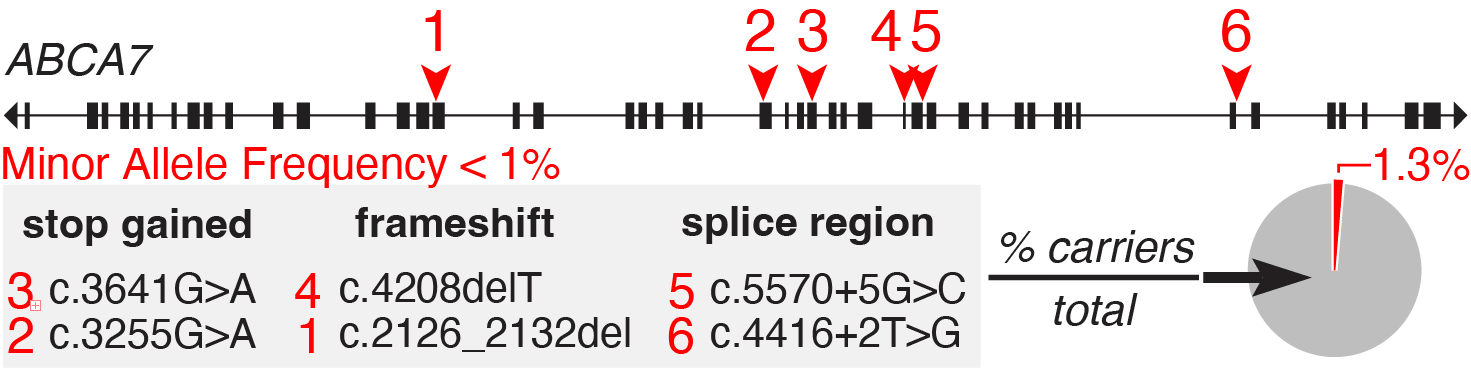
\includegraphics[width=\textwidth]{./main_plots/abca7_variants_cartoon.png}        
    \end{subfigure}
    \begin{subfigure}[t]{.55\textwidth}
        \caption{}
        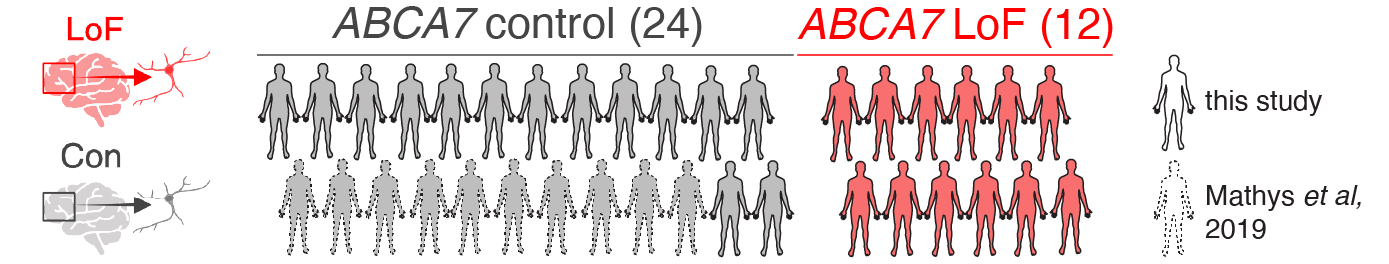
\includegraphics[width=\textwidth]{./main_plots/cohort_cartoon.png}        
    \end{subfigure}
    \\[-1ex] 
    \begin{subfigure}[t]{.5\textwidth}
        \begin{subfigure}[t]{\textwidth}
            \caption{}
            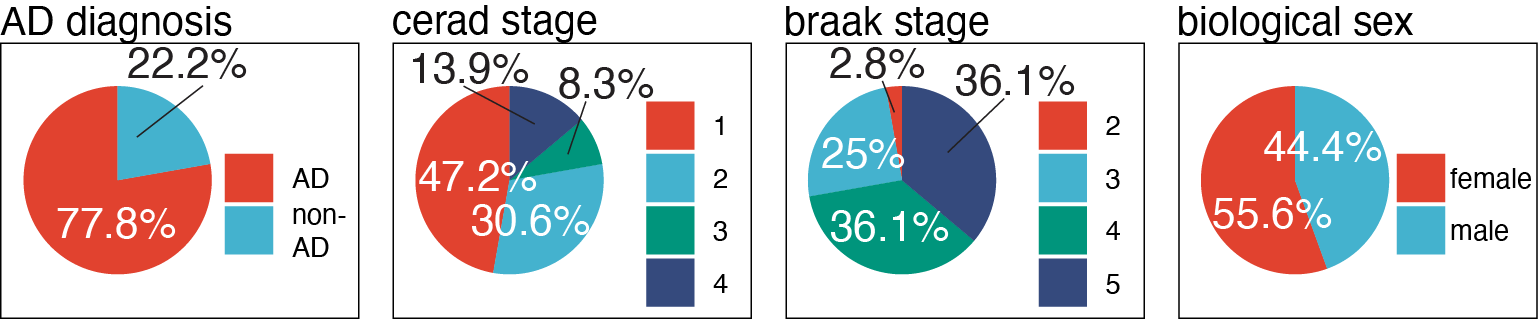
\includegraphics[width=\textwidth]{./main_plots/pie_charts.png}        
        \end{subfigure}
        \begin{subfigure}[t]{.45\textwidth}
            \caption{}
            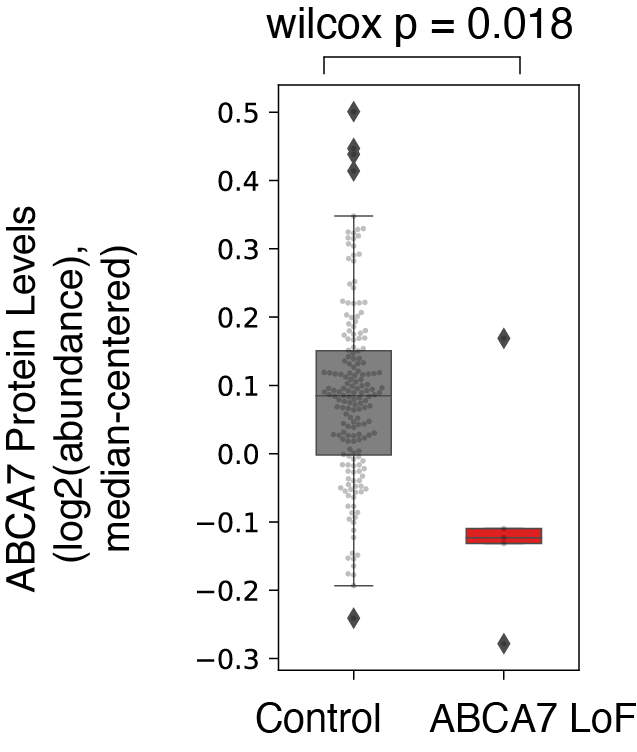
\includegraphics[width=\textwidth]{./main_plots/abca7_protein_levels.png}        
        \end{subfigure}
        \begin{subfigure}[t]{.5\textwidth}
            \caption{}
            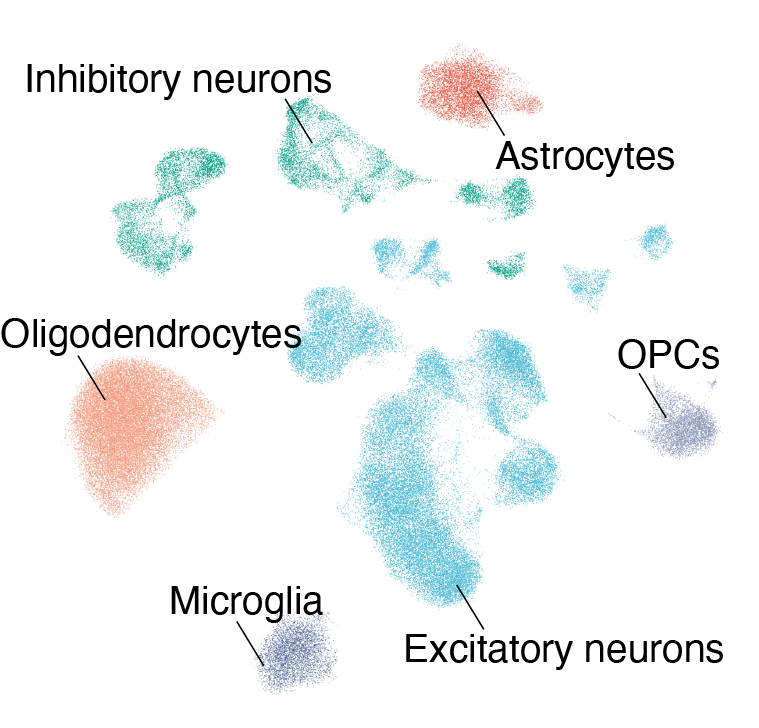
\includegraphics[width=\textwidth]{./main_plots/cell_projection.png}        
        \end{subfigure}
    \\[-3ex] 
    \end{subfigure}
    \begin{subfigure}[t]{0.5\textwidth}
        \caption{}
        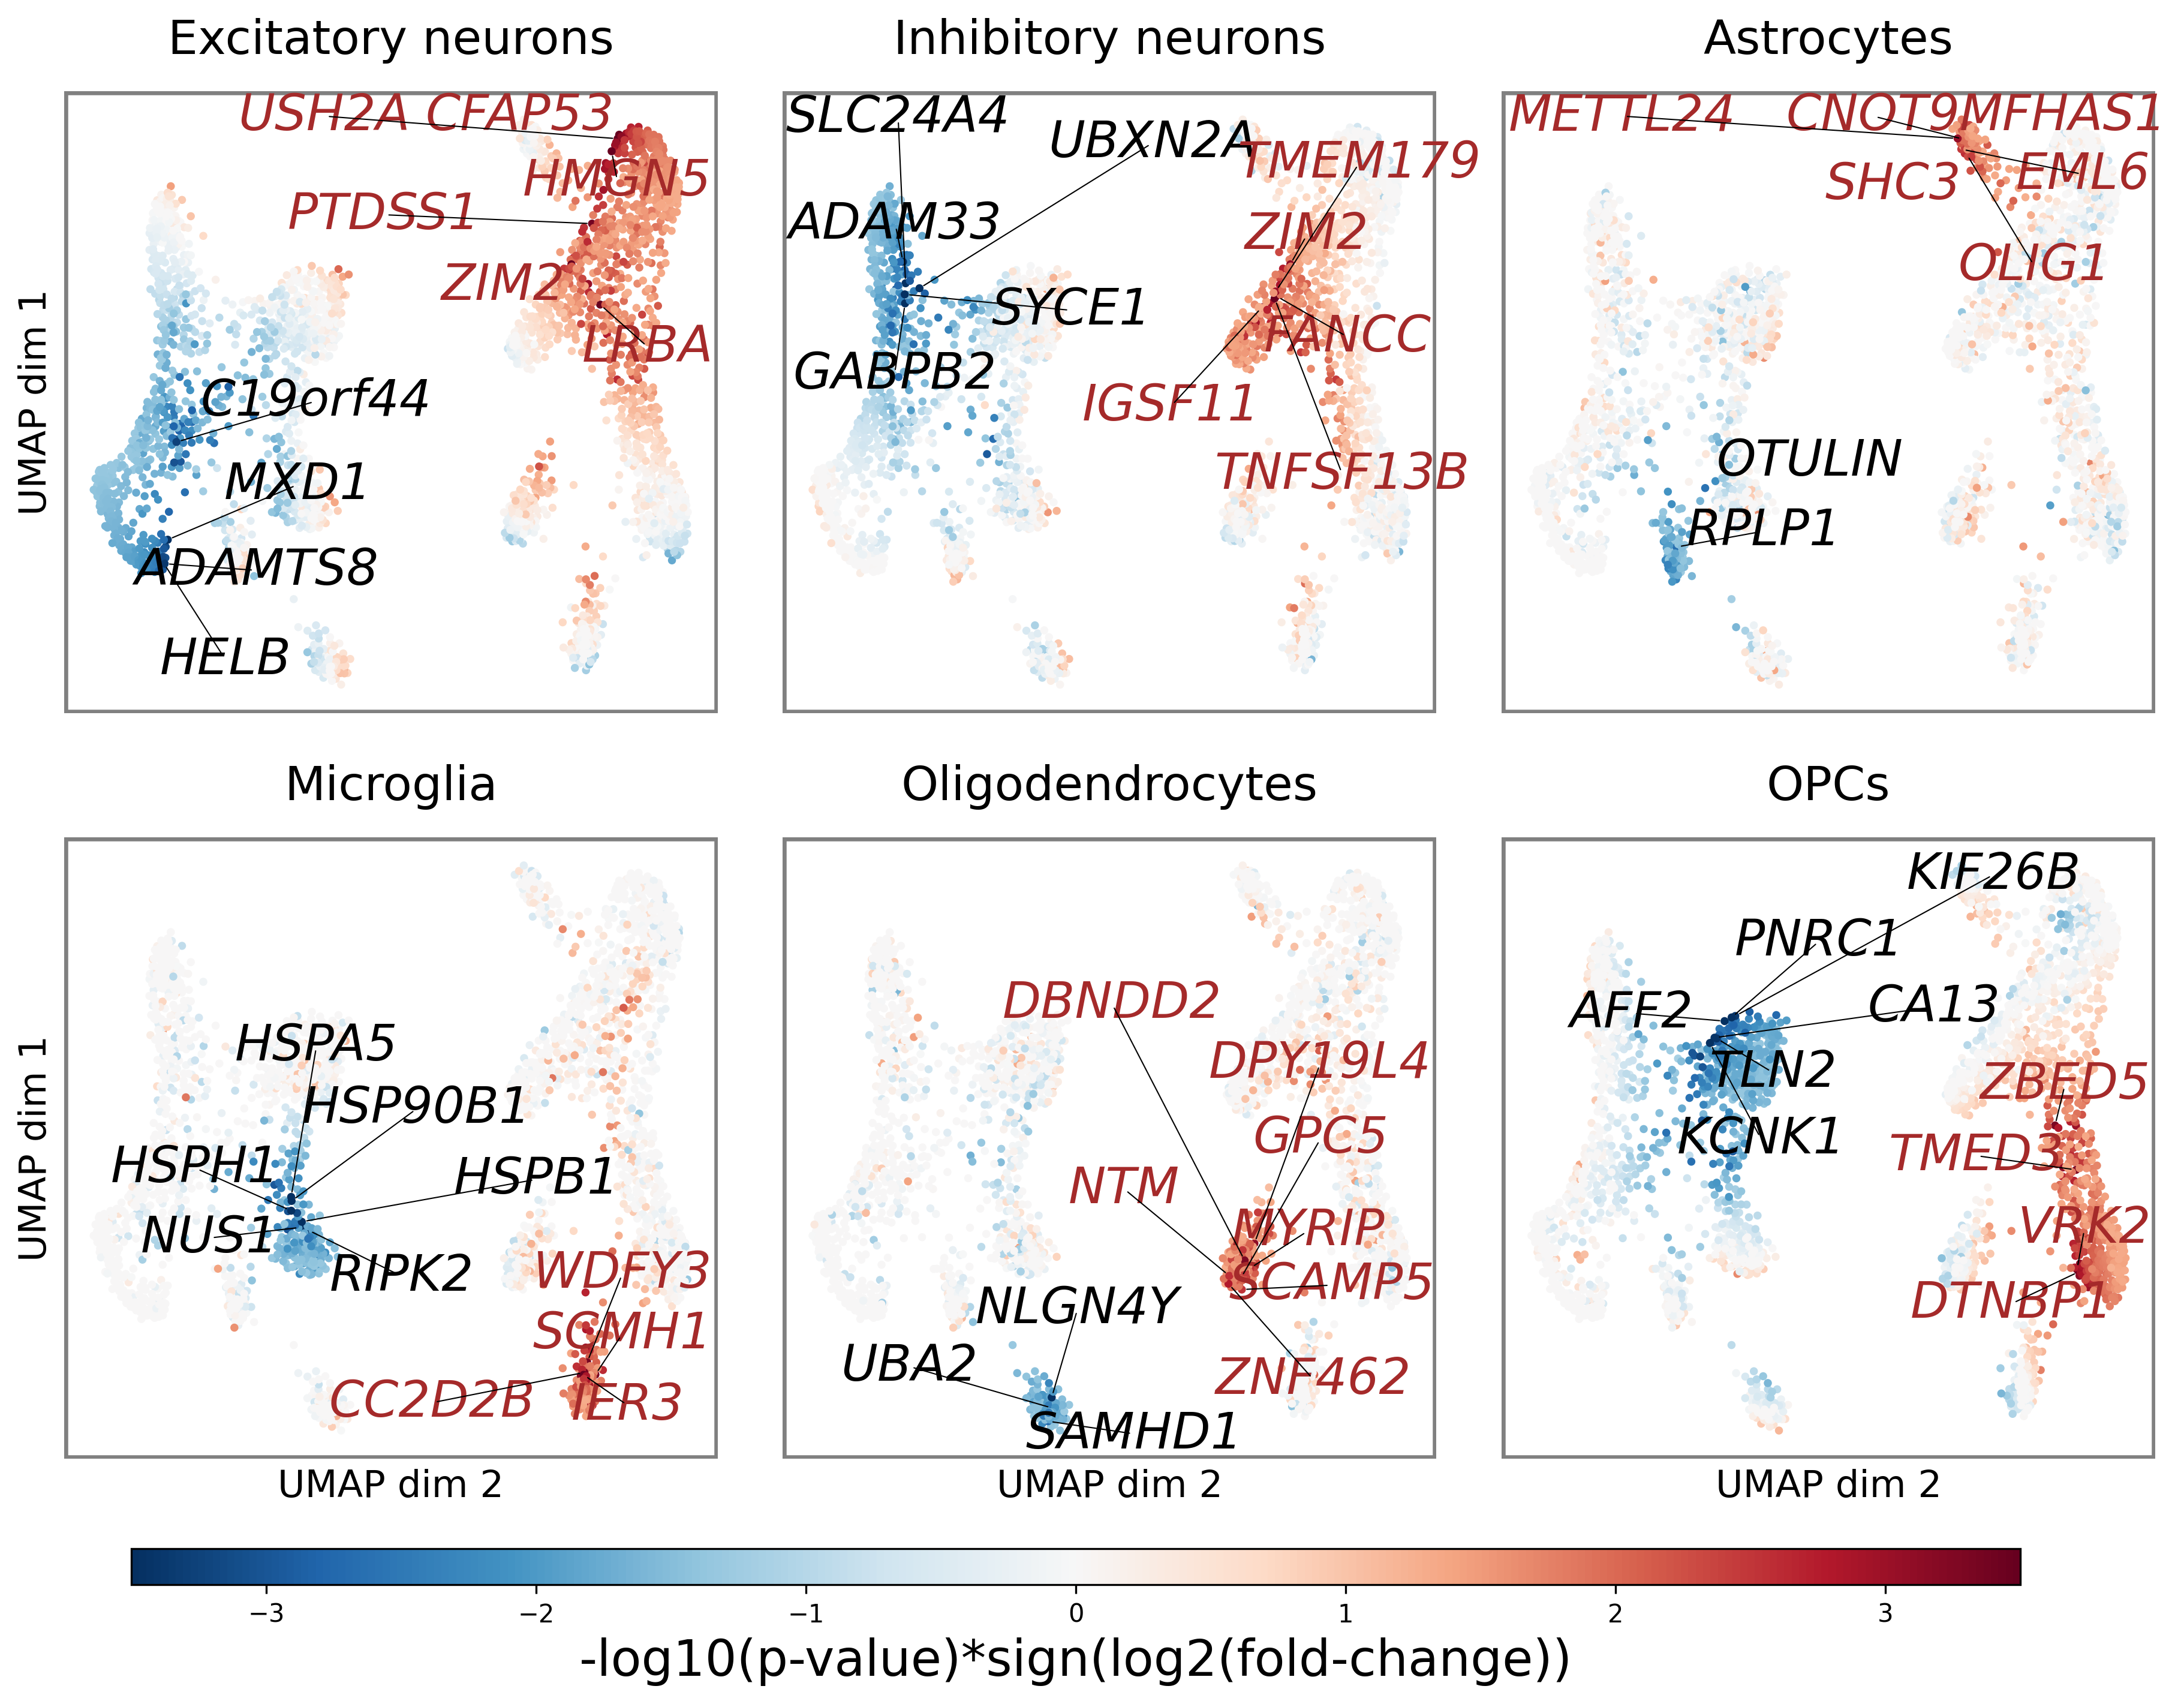
\includegraphics[width=\textwidth]{./main_plots/umap_projection_top_genes.png}        
    \end{subfigure}
    \begin{subfigure}[t]{\textwidth}
        \caption{}
        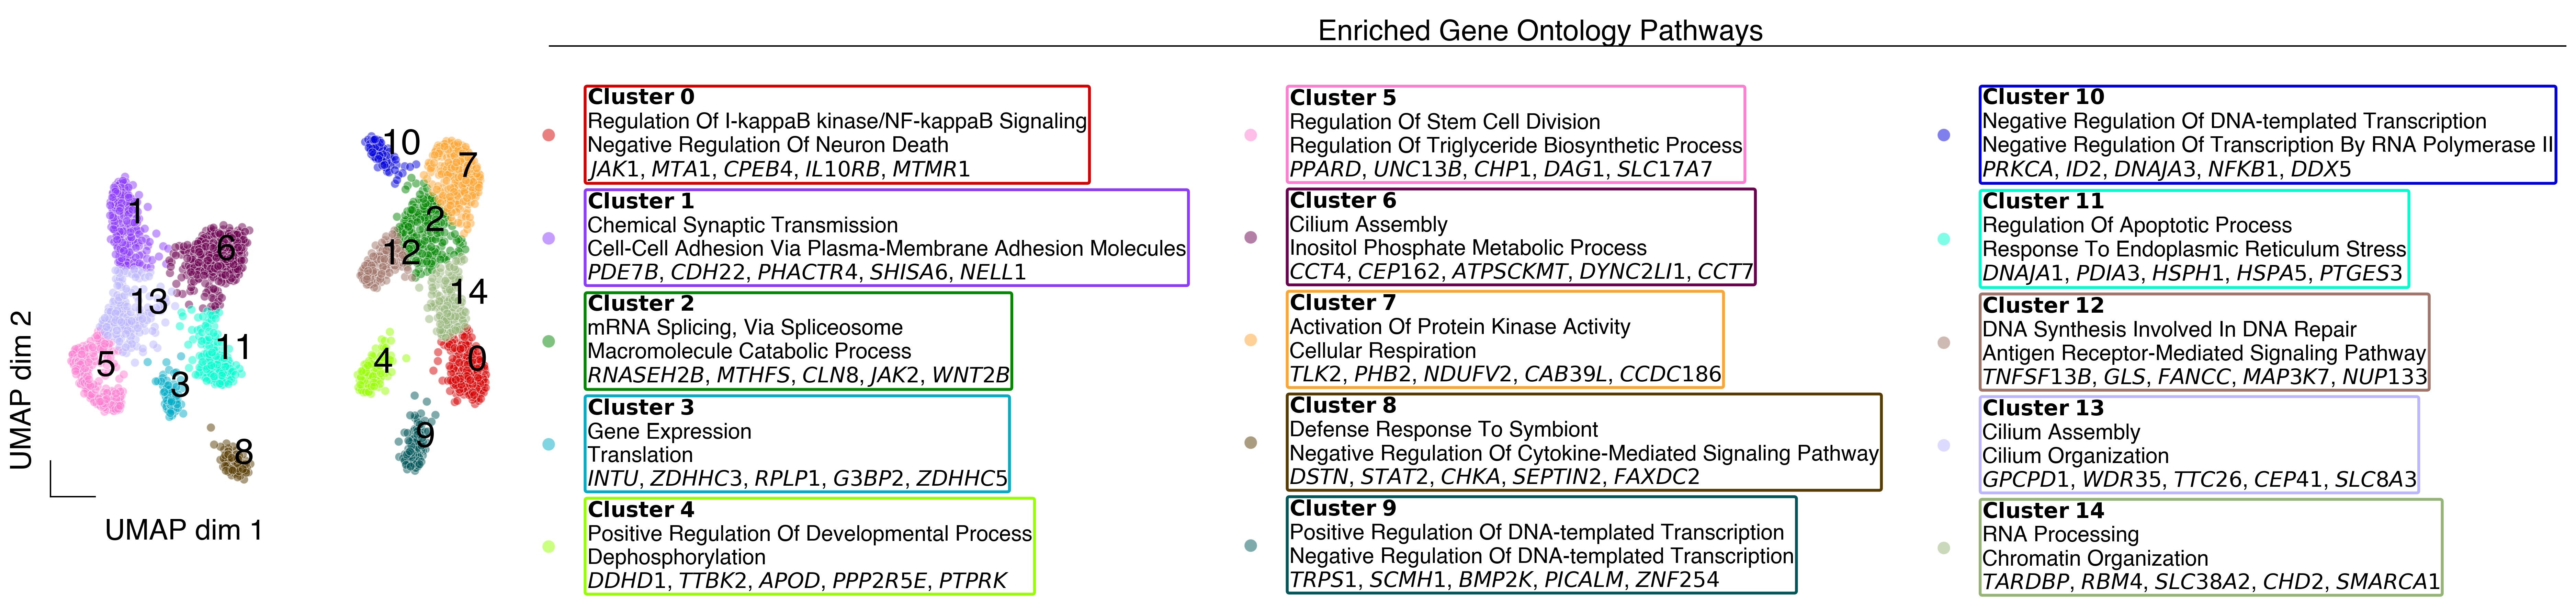
\includegraphics[width=\textwidth]{./main_plots/clusters_umap.png}        
    \end{subfigure}
    \\[-2ex] 
    \begin{subfigure}[t]{\textwidth}
        \caption{}
        
\includegraphics[width=\textwidth]{./main_plots/clusters_bars.png}        
    \end{subfigure}
    \caption{
        \textbf{Single-nuclear RNA-sequencing Atlas of Human Post-mortem Prefrontal Cortex Reveals Cell Type-specific Gene Changes in ABCA7 LoF.}\\
        }
    \label{fig:main_atlas}
\end{figure}
\begin{itemize}
\item[\textbf{(A)}] Overview of ABCA7 gene structure with the location of variants represented in this study (average minor allele frequency for depicted variants is < 1\%). Exons are depicted as black rectangles, and introns as black lines. The pie chart indicates the frequency of ABCA7 PTC-variant-carriers within the ROSMAP cohort. 
\item[\textbf{(B)}] Overview of human cohort for snRNA-seq (Created with BioRender.com). 
\item[\textbf{(C)}] Overview of snRNA-seq cohort metadata for 32 individuals. 
\item[\textbf{(D)}] ABCA7 protein levels (log2(abundance)) from post-mortem human prefrontal cortex in all available controls ($N=180$) vs. ABCA7 LoF carriers ($N=5$). P-value computed by Wilcoxon rank sum test. Boxes indicate per-condition dataset quartiles, and whiskers extend to the most extreme data points not considered outliers (i.e., within 1.5 times the interquartile range from the first or third quartile). 
\item[\textbf{(E)}] 2D UMAP projection of per-cell gene expression values and their transcriptionally defined cell type. 
\item[\textbf{(F)}] 2D UMAP projection of ABCA7 LoF gene perturbation scores ($S = -\log_{10}(\text{p-value}) \times \text{sign}(\log_2(\text{fold change}))$); Red = $S>1.3$, Blue = $S<-1.3$; Point size indicates $|S|$). Up to top 20 genes by $|S|$ are labeled. 
\item[\textbf{(G)}] Genes in 2D UMAP space colored by cluster assignment (Gaussian mixture model; see Methods) with per-cluster pathway enrichments shown (GO BP, hypergeometric enrichment, $p<0.01$). 
\item[\textbf{(H)}] Cell type-specific gene cluster scores ($SC = \text{mean}(S_i)$, for genes $i$ in cluster $c$). * indicates permutation FDR-adjusted p-value $< 0.01$ and $|SC| > 0.25$.
\end{itemize}
\clearpage

\begin{figure}[H]
    \begin{subfigure}[t]{0.45\textwidth}
        \begin{subfigure}[t]{0.49\textwidth}
            \caption{}
            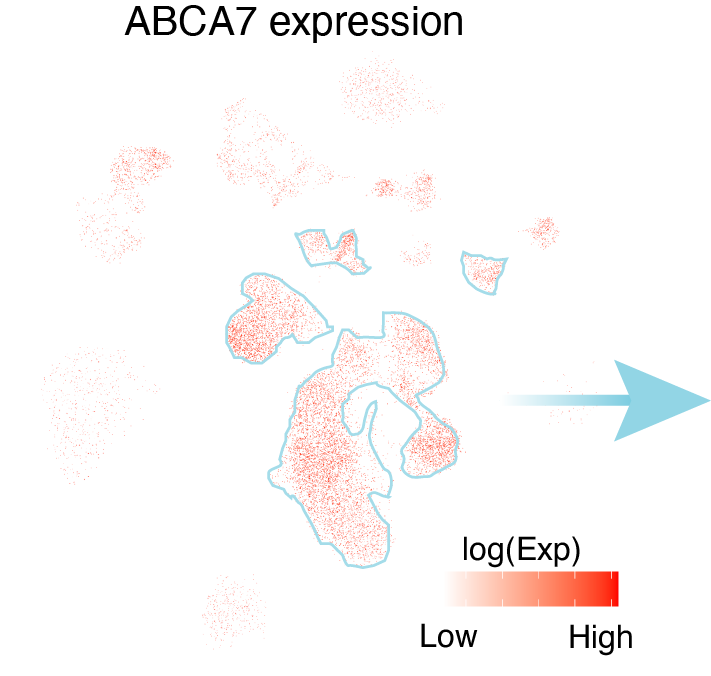
\includegraphics[width=\textwidth]{./main_plots/cell_projection_abca7_expression.png}        
        \end{subfigure}
        \begin{subfigure}[t]{0.49\textwidth}
            \caption{}
            \includegraphics[width=\textwidth]{./main_plots/pm_kl_network_network.pdf}        
        \end{subfigure}
        \begin{subfigure}[t]{\textwidth}
            \caption{}
            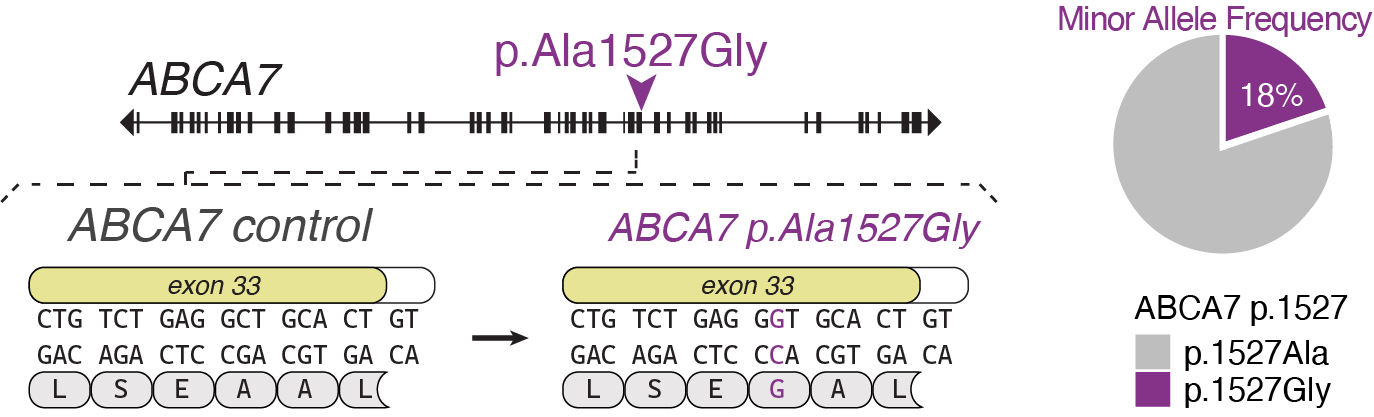
\includegraphics[width=\textwidth]{./main_plots/common_variant_cartoon.png}        
        \end{subfigure}
    \end{subfigure}
    \begin{subfigure}[t]{0.45\textwidth}
        \caption{}
        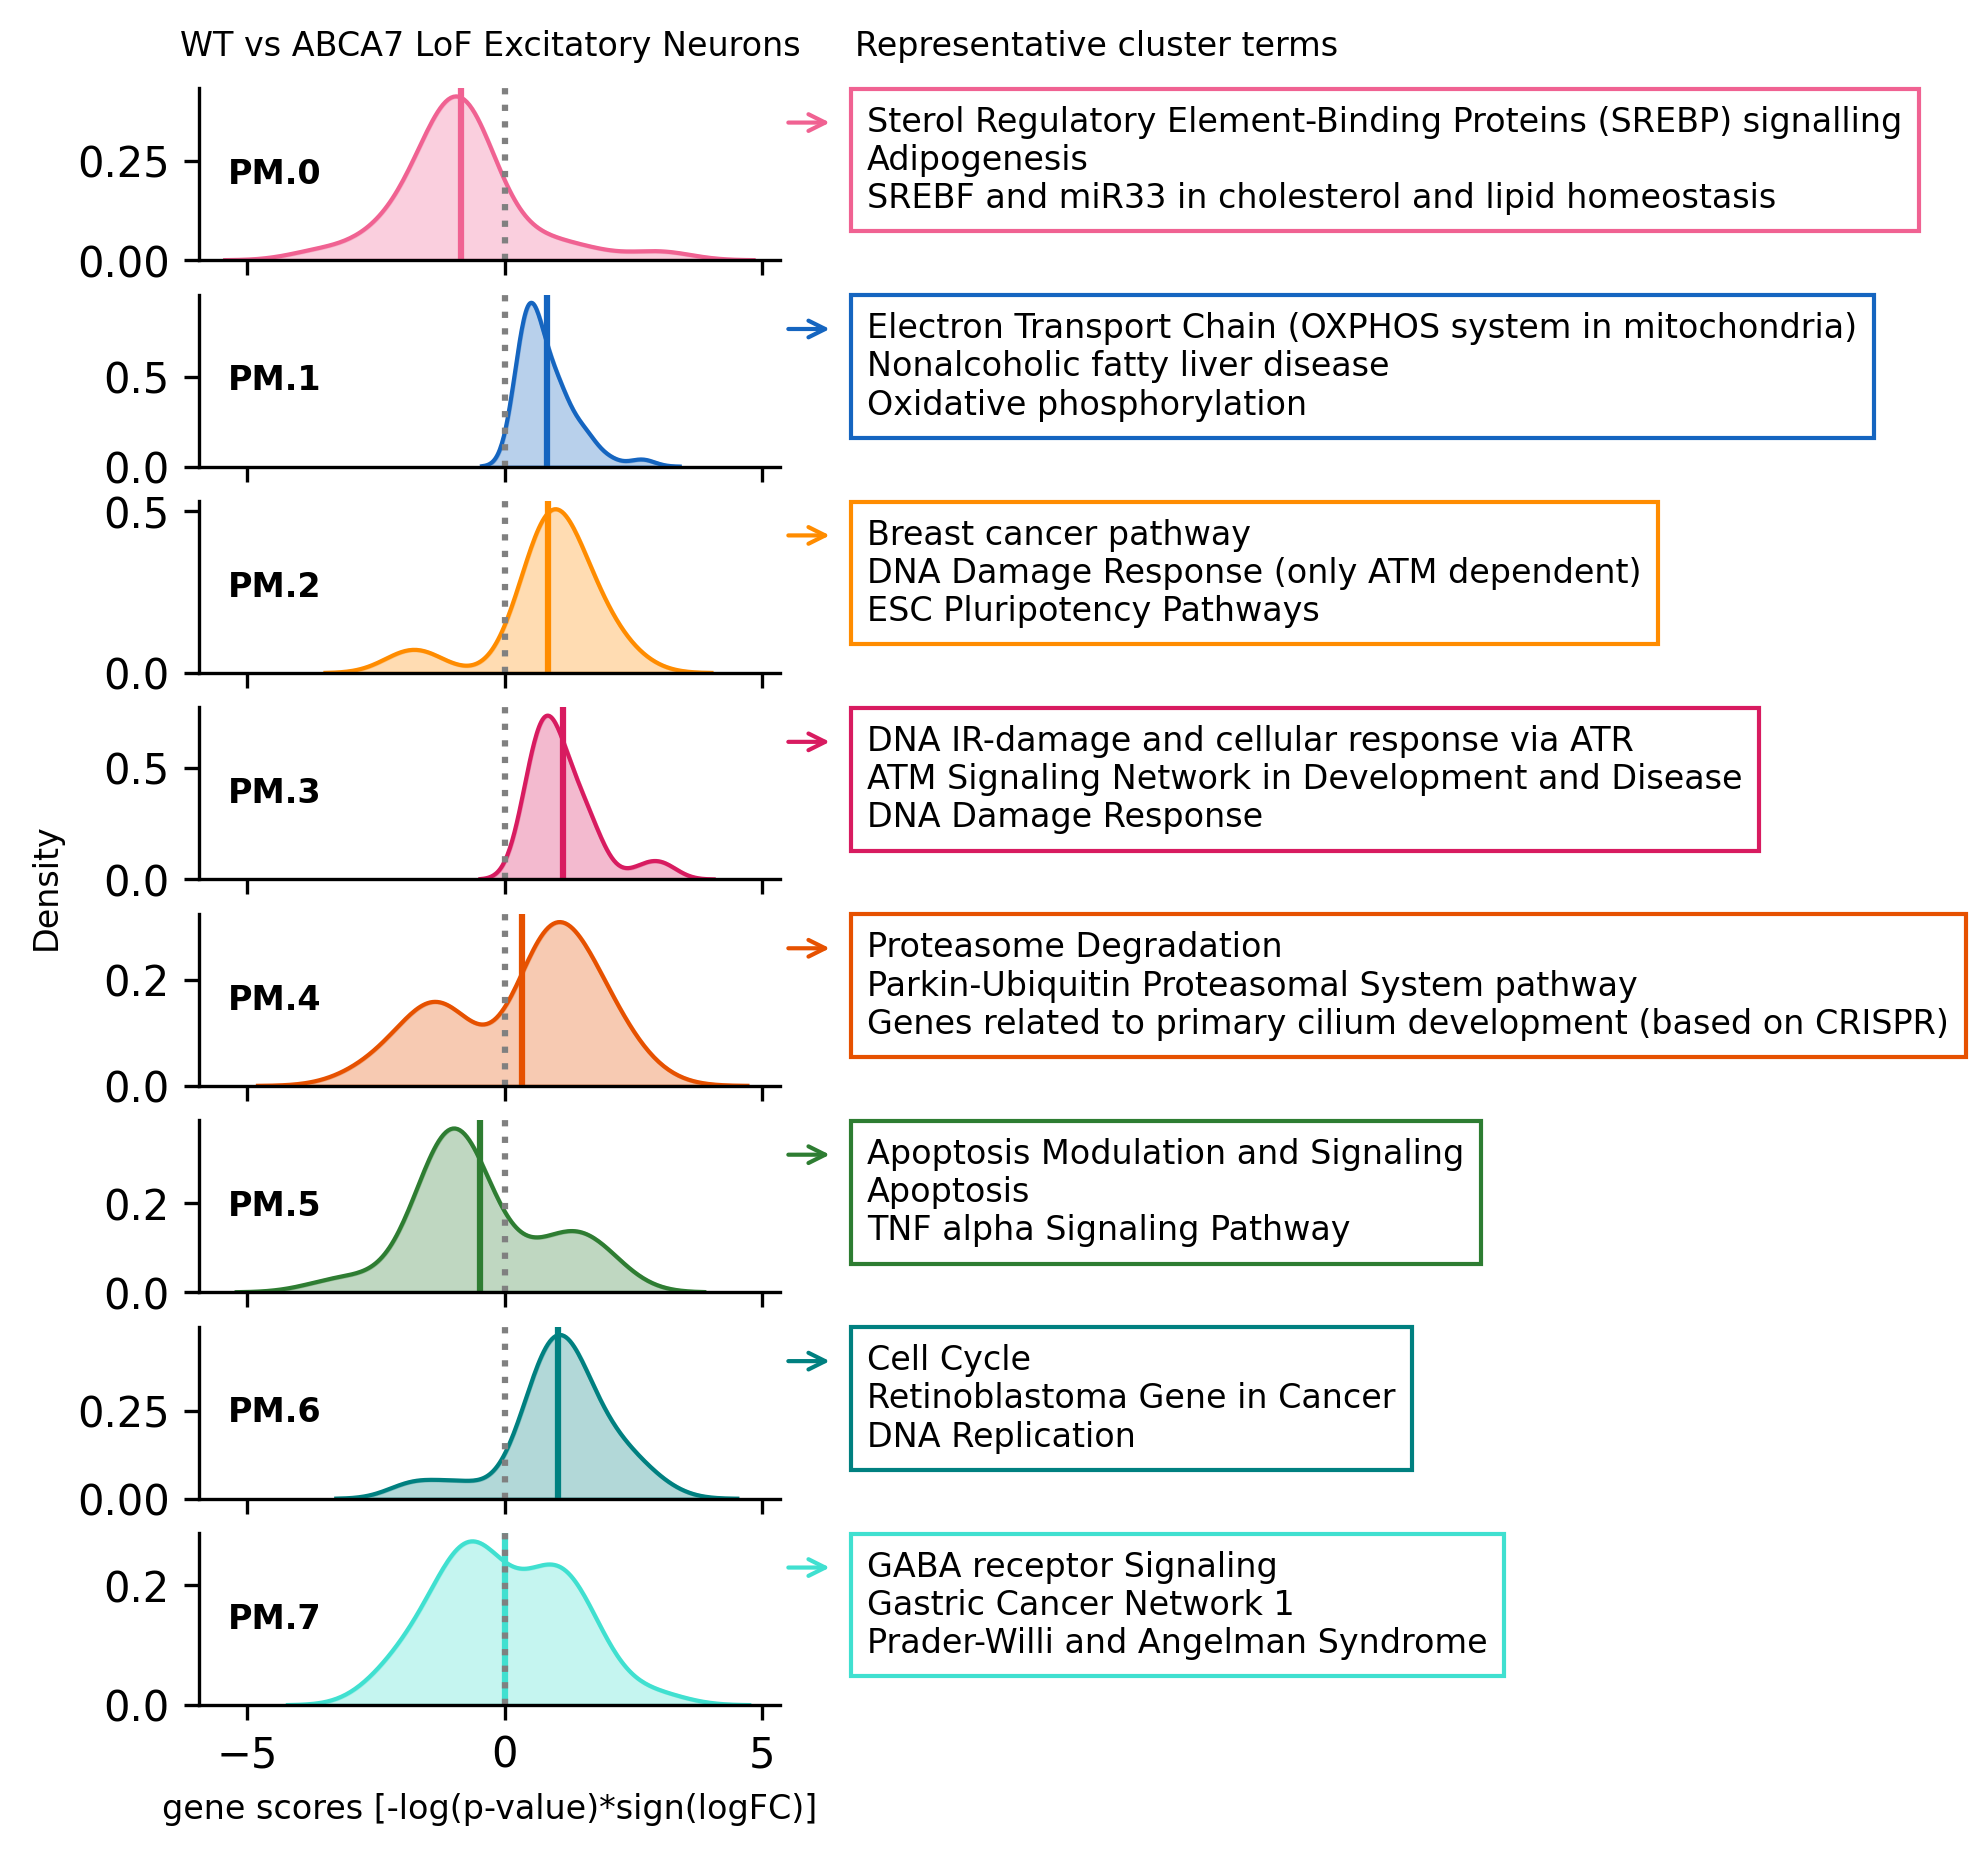
\includegraphics[width=\textwidth]{./main_plots/kl_densities.png}        
    \end{subfigure}
    \begin{subfigure}[t]{0.3\textwidth}
        \caption{}
        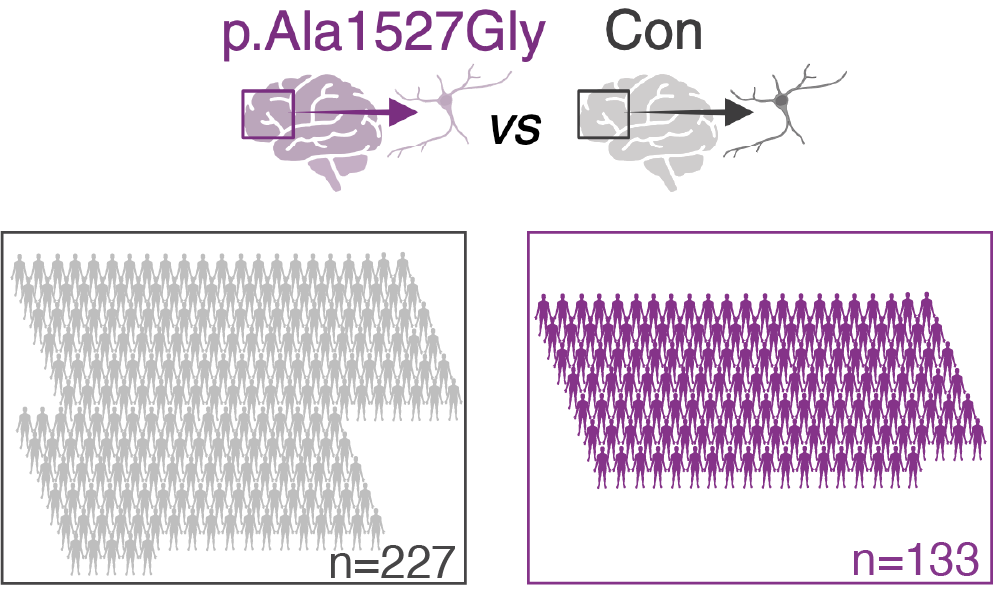
\includegraphics[width=\textwidth]{./main_plots/common_var_cohort_cartoon.png}        
    \end{subfigure}
    \hspace{0.01\textwidth} % Adjust this value as needed
    \begin{subfigure}[t]{0.225\textwidth}
        \caption{}
        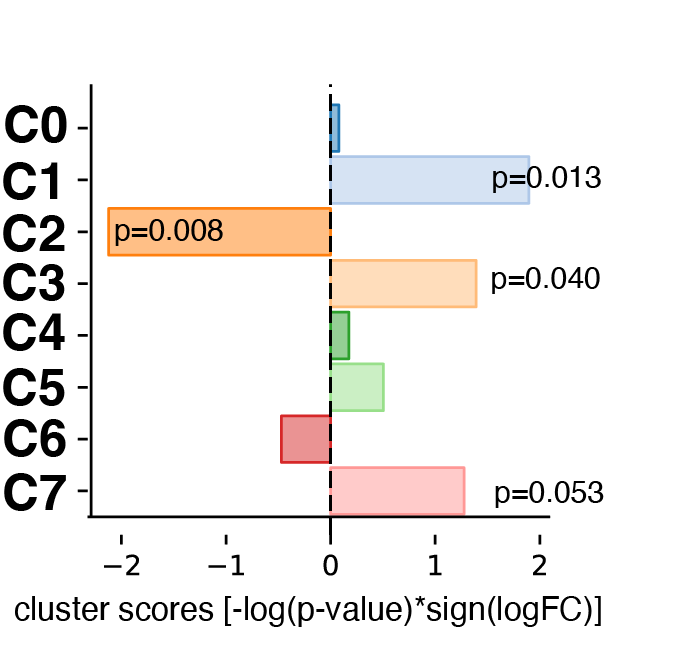
\includegraphics[width=\textwidth]{./main_plots/variant_path_scores.png}        
    \end{subfigure}
    \begin{subfigure}[t]{0.45\textwidth}
        \caption{}
        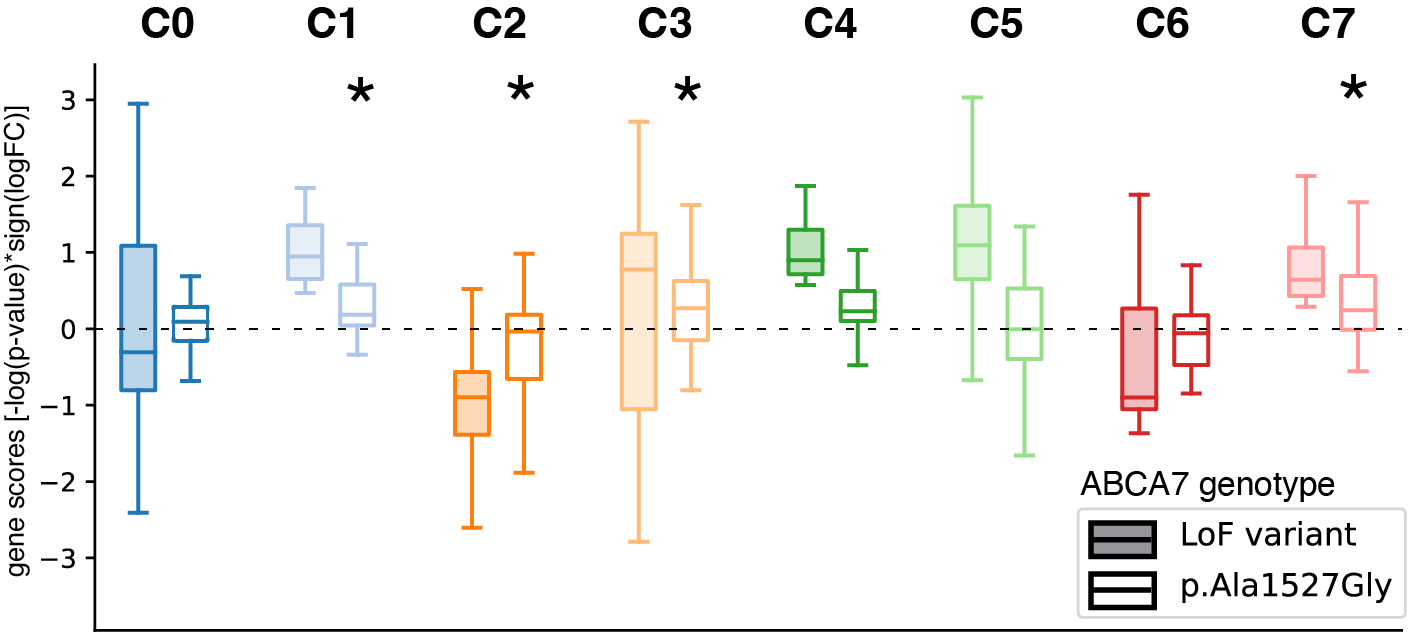
\includegraphics[width=\textwidth]{./main_plots/common_var_distributions.png}        
    \end{subfigure}
    \begin{subfigure}[t]{0.3\textwidth}
        \caption{}
        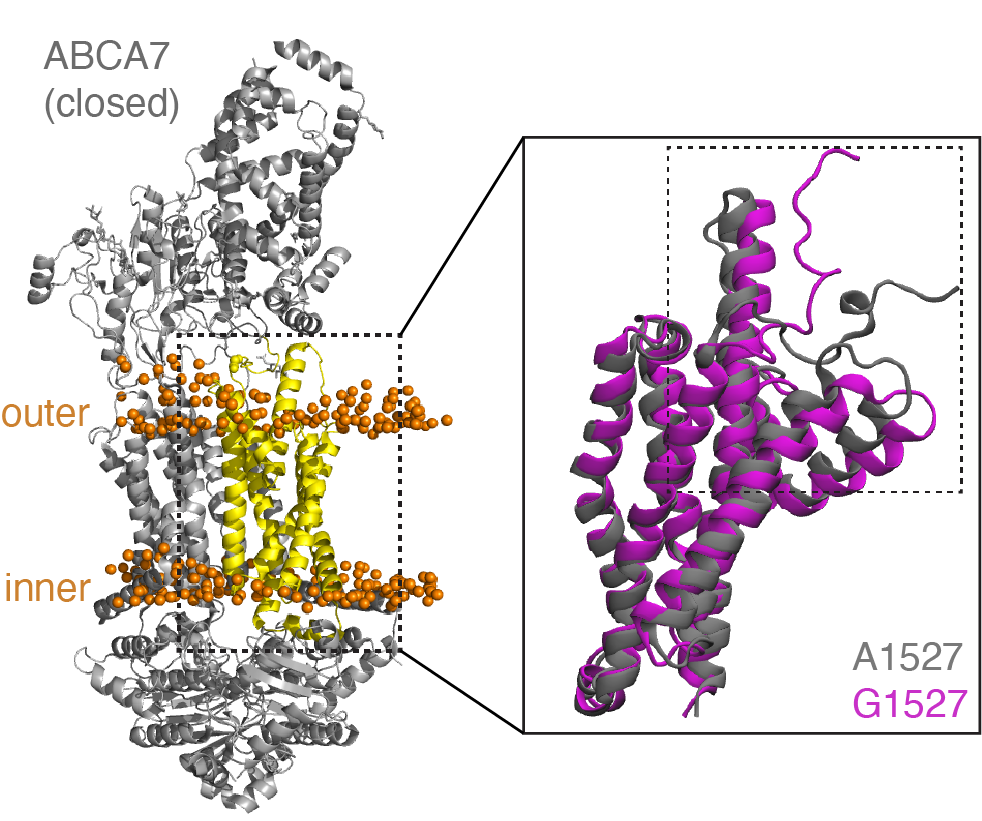
\includegraphics[width=\textwidth]{./main_plots/abca7_structure_with_inset.png}        
    \end{subfigure}
    \begin{subfigure}[t]{0.165\textwidth}
        \caption{}
        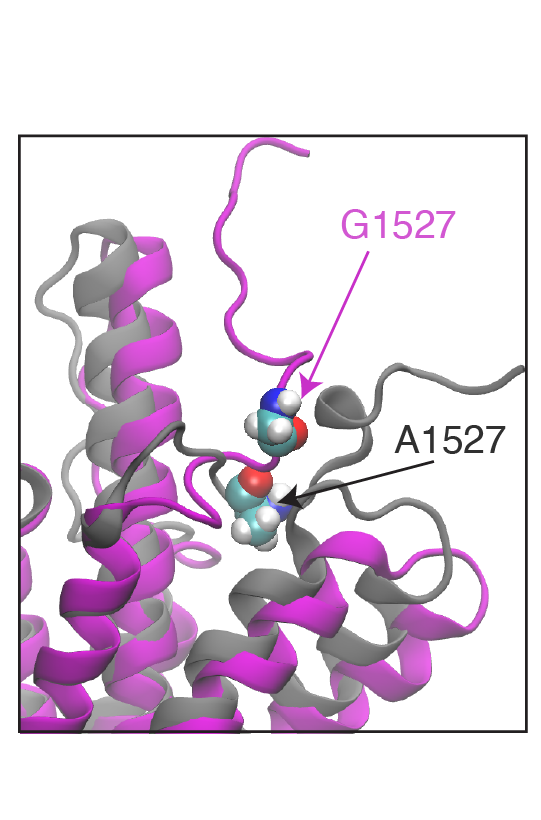
\includegraphics[width=\textwidth]{./main_plots/abca7_inset_only.png}        
    \end{subfigure}
    \hspace{0.01\textwidth} % Adjust this value as needed
    \begin{subfigure}[t]{0.32\textwidth}
        \caption{}
        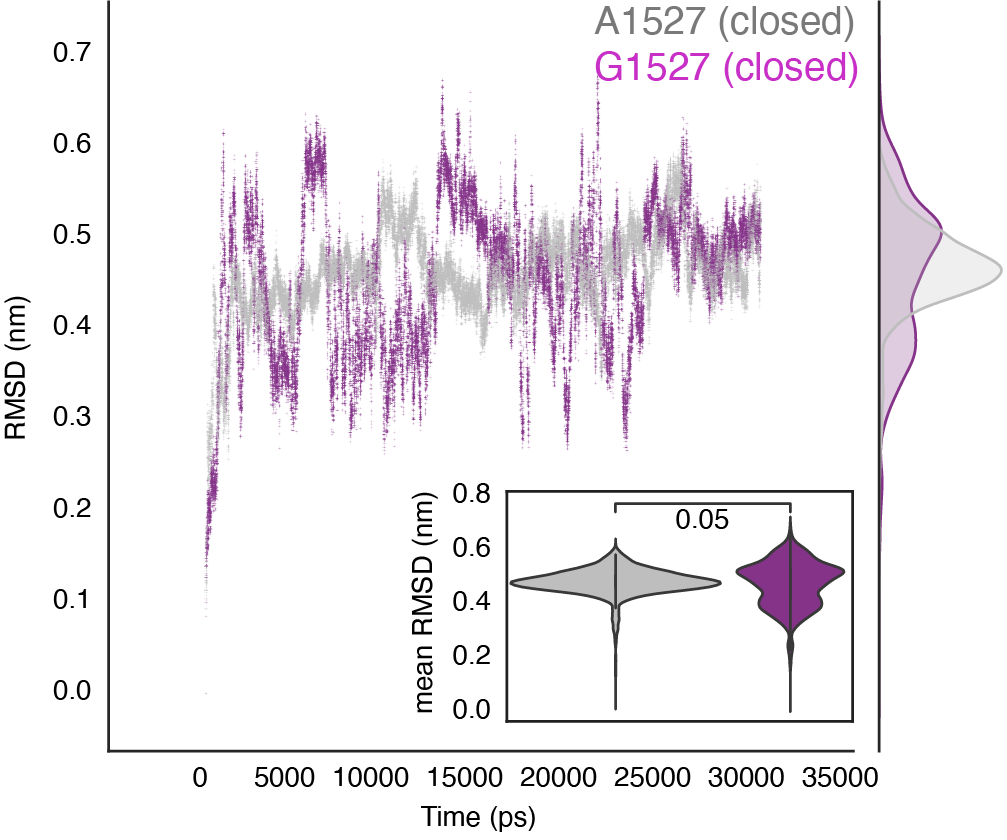
\includegraphics[width=\textwidth]{./main_plots/variant_dynamics.png}        
    \end{subfigure}
    \begin{subfigure}[t]{0.16\textwidth}
        \caption{}
        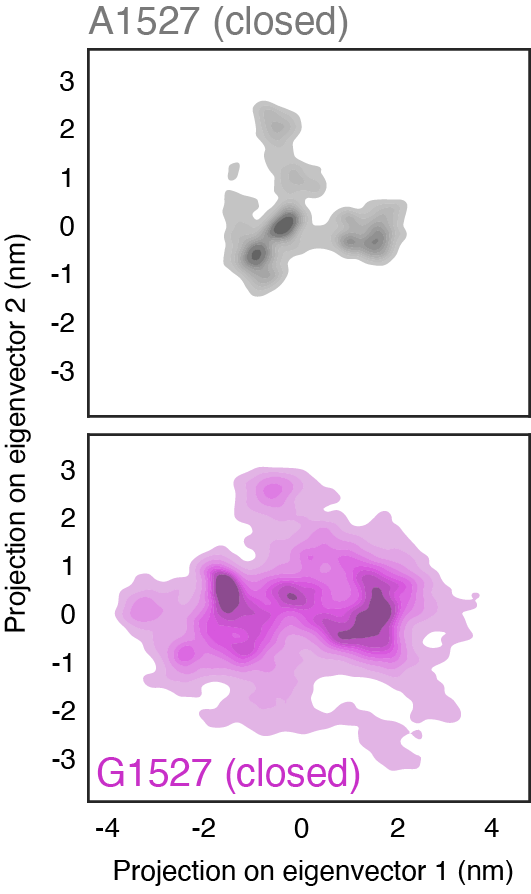
\includegraphics[width=\textwidth]{./main_plots/variant_projection_closed.png}        
    \end{subfigure}
    \caption{
        \textbf{Transcriptional Perturbations in Excitatory Neurons in ABCA7 LoF and ABCA7 p.Ala1527Gly Variant Carriers.}\\
    }
    \label{fig:main_neurons}
\end{figure}
\begin{itemize}
    \item[\textbf{(A)}] 2D UMAP projection of individual cells colored by log(Exp), where Exp represents log-normalized ABCA7 expression values.
    \item[\textbf{(B)}] Kernighan-Lin (K/L) clustering on leading edge genes from pathways perturbed in ABCA7 LoF excitatory neurons, where $p<0.05$. Colors indicate distinct K/L gene clusters, which are numbered from 0 to 7.
    \item[\textbf{(C)}] Left: Gaussian kernel density estimate plots of gene scores $S$ for genes belonging to a given gene cluster. $S>0$ indicates upregulation in ABCA7 LoF. Solid lines indicate distribution means. Right: Representative pathways that annotate the largest number of genes within a cluster (i.e., with the highest intra-cluster connectivity) shown per-cluster. 
    \item[\textbf{(D)}] Schematic indicating the genomic location of the p.Ala1527Gly codon change. A purple arrow indicates the location of the missense variant in the ABCA7 gene. Minor allele frequency shown to the right. 
    \item[\textbf{(E)}] Overview of snRNA-seq cohort of ABCA7 p.Ala1527Gly carriers (homozygous and heterozygous) vs. control non-carriers (minor allele frequency approx. 18\%).
    \item[\textbf{(F)}] Perturbation of ABCA7 LoF-associated gene clusters from (B-D) in excitatory neurons of p.Ala1527Gly variant-carriers vs. non-carrier controls, computed by FGSEA. Top $p$-values ($p<0.1$) are indicated. $S>0$ indicates upregulation in carriers.
    \item[\textbf{(G)}] Distributions of gene scores $S$ for genes belonging to a given gene cluster for ABCA7 p.Ala1527Gly (no fill) or ABCA7 LoF-variants (solid fill). $S>0$ indicates upregulation in ABCA7 variant. * indicates FGSEA $p$-value<0.1 from (G). Boxes indicate per-condition dataset quartiles, and whiskers extend to the most extreme data points not considered outliers (i.e., within 1.5 times the interquartile range from the first or third quartile).
    \item[\textbf{(H)}] Closed conformation ABCA7 protein structure. ABCA7 domain between residues 1517 and 1756 used for simulations is shown in yellow. Lipid bilayer shown in orange. Expanded yellow domain shown in inset, with A1527 variant (light grey) and G1527 variant (purple).
    \item[\textbf{(I)}] Expanded inset from H with residues of interest rendered.
    \item[\textbf{(J)}] Root mean squared deviations of closed conformation domains from I with A1527 (light grey) or G1527 (purple) under simulation. Structural deviations over time were computed with respect to reference closed conformation from I. Violin plot inset indicates average $C_\alpha$ atom positional fluctuations over time.
    \item[\textbf{(K)}] Projection of $C_\alpha$ atom positional fluctuations under simulation onto the first two principal components, for closed conformation domain from J with A1527 (top, light grey) or G1527 (bottom, purple). 
\end{itemize}
\clearpage

\begin{figure}[H]
    % ROW 1
    
    \begin{subfigure}[t]{.24\textwidth}
        \begin{subfigure}[t]{\textwidth}
            \caption{}
            \includegraphics[width=\textwidth]{./main_plots/iN_gen2.png}        
            \includegraphics[width=\textwidth]{./extended_plots/variant_locations.png}        
            \includegraphics[width=\textwidth]{./main_plots/iN_rep_ims.png}        
        \end{subfigure} 
        \begin{subfigure}[t]{\textwidth}
            \caption{}
            \includegraphics[width=\textwidth]{./extended_plots/rna_correlation_both_lof_lines.png}        
        \end{subfigure} 
    \end{subfigure} 
    \hspace{.5cm}
    \begin{subfigure}[t]{.23\textwidth}
        \begin{subfigure}[t]{\textwidth}
            \caption{}
            \includegraphics[width=\textwidth]{./main_plots/y622_kl_clusters_network.pdf}        
        \end{subfigure}
        \begin{subfigure}[t]{\textwidth}
            \caption{}
            \centering
            \includegraphics[width=0.5\textwidth]{./main_plots/jaccard_cartoon.png}        
            \includegraphics[width=\textwidth]{./main_plots/jaccard_PM_pT622.png}        
        \end{subfigure}  
    \end{subfigure} 
    \hspace{.25cm}
    \begin{subfigure}[t]{.45\textwidth}
        \caption{}
        \includegraphics[width=\textwidth]{./main_plots/kl_densities_Tyr622.png}        
    \end{subfigure}  
    % Row 2
    \vspace{.25cm}
    \begin{subfigure}[t]{.25\textwidth}
        \begin{subfigure}[t]{\textwidth}
            \caption{}
            \includegraphics[width=\textwidth]{./main_plots/y622_mito_degs.png}        
        \end{subfigure}  
    \end{subfigure} 
    \begin{subfigure}[t]{.2\textwidth}
        \caption{}
            \includegraphics[width=\textwidth]{./main_plots/uncoupling.png}        
    \end{subfigure}   
    \begin{subfigure}[t]{.5\textwidth}
        \caption{}
        \includegraphics[width=\textwidth]{./extended_plots/mitohealth_y_g.png}        
    \end{subfigure}    
    % Row 3
    \begin{subfigure}[t]{.35\textwidth}
        \caption{}
        \includegraphics[width=\textwidth]{./main_plots/tmrm_main.png}        %tmrm_with_FCCP
    \end{subfigure}    
   % \hspace{1cm}
    \hspace{.25cm}
    \begin{subfigure}[t]{.35\textwidth}
        \caption{}
        \includegraphics[width=\textwidth]{./main_plots/cellrox_images.png}        
    \end{subfigure}  
    \hspace{.5cm}
    \begin{subfigure}[t]{.2\textwidth}
        \caption{}
        \includegraphics[width=\textwidth]{./main_plots/all_lipids_y622.png}        
    \end{subfigure}  
    \caption{
        \textbf{ABCA7 LoF Impairs Regulation of Mitochondrial Uncoupling in Neurons.}\\
    }
    \label{fig:main_mitochondrial}
\end{figure}
\begin{itemize}
\item[\textbf{(A)}] Schematic of iPSC-derived isogenic neuronal lines carrying ABCA7 LoF variants. The ABCA7 gene map highlights exons (black rectangles) and introns (black lines). CRISPR-Cas9 was used to introduce a premature termination codon in exon 3 (p.Glu50fs3, blue) or exon 15 (p.Tyr622, orange).\\
\item[\textbf{(B)}] Correlation of per-gene perturbation scores ($S = -\log_{10}(\text{p-value}) \times \text{sign}(\log_2(\text{fold change}))$) between p.Glu50fs3 vs. WT and p.Tyr622 vs. WT iNs.\\
\item[\textbf{(C)}] Kernighan-Lin (K/L) clustering of leading-edge genes from pathways perturbed in p.Tyr622* vs. WT iNs (p-adjusted < 0.05). Colors indicate distinct K/L gene clusters, which are assigned postmortem (PM) cluster labels if they significantly overlap with PM-identified clusters based on Jaccard analysis in (D). Otherwise, they are labeled with a 'T' prefix.\\
\item[\textbf{(D)}] Heatmap showing Jaccard index-based overlap between K/L clusters from p.Tyr622* vs. WT iNs and postmortem-identified clusters.\\
\item[\textbf{(E)}] Left: Gaussian kernel density estimate plots of gene scores $S$ for genes within each cluster ($S>0$ indicates upregulation in ABCA7 LoF). Solid lines represent distribution means. Right: Top representative pathways associated with the highest intra-cluster connectivity.\\
\item[\textbf{(F)}] Volcano plot of differentially expressed genes between p.Tyr622* and WT iNs, highlighting genes with mitochondrial localization.\\
\item[\textbf{(G)}] Uncoupled mitochondrial oxygen consumption rate (OCR) in WT vs. ABCA7 LoF iNs, measured by Seahorse assay. P-values computed via independent sample t-test. $N$ wells = 18 (WT), 17 (p.Tyr622*), 13 (p.Glu50fs*3) from two independent differentiation batches.\\
\item[\textbf{(H)}] Left: Quantification of mitochondrial membrane potential using HCS MitoHealth dye in neurons. P-values computed using a linear mixed-effects model on per-NeuN+ volume averages, with well-of-origin as a random effect. $N=8$ (WT), 11 (p.Tyr622*), 9 (p.Glu50fs*3), with ~3000 cells per condition from three independent differentiation batches. Right: Representative images showing NeuN+ cells and corresponding MitoHealth and Hoechst staining. MitoHealth images underwent percentile-based background subtraction and thresholding.\\
\item[\textbf{(I)}] Average TMRM fluorescence intensity in p.Tyr622* vs. WT iNs per mask (binarized TMRM signal based on the 75th percentile threshold) under baseline conditions and after FCCP treatment.\\
\item[\textbf{(J)}] Average CellROX fluorescence intensity in p.Tyr622* vs. WT iNs per mask (binarized CellROX signal based on the 75th percentile threshold).\\
\item[\textbf{(K)}] Volcano plot of differentially abundant lipid species between p.Tyr622* and WT iNs, colored by lipid class.
\end{itemize}
\clearpage

\begin{figure}[H]
%    \includegraphics[width=\textwidth]{./main_plots/fig_5_temp.png}
    \begin{subfigure}[t]{.24\textwidth}
        \begin{subfigure}[t]{\textwidth}
            \caption{}
            \includegraphics[width=\textwidth]{./main_plots/all_lipids_choline_batch1.png}        
        \end{subfigure} 
        \begin{subfigure}[t]{\textwidth}
            \caption{}
            \vspace{-0.5cm}
            \centering
            \includegraphics[width=.8\textwidth]{./main_plots/rna_correlation_plot.png}        
        \end{subfigure}  
    \end{subfigure}  
    \hspace{.5cm}
    \begin{subfigure}[t]{.23\textwidth}
        \begin{subfigure}[t]{\textwidth}
            \caption{}
            \includegraphics[width=\textwidth]{./main_plots/Y622_choline_kl_network_network.pdf}        
        \end{subfigure}  
        \begin{subfigure}[t]{\textwidth}
            \caption{}
            \includegraphics[width=\textwidth]{./main_plots/jaccard_pT622_with_choline.png}        
        \end{subfigure} 
    \end{subfigure} 
    \hspace{.25cm}
    \begin{subfigure}[t]{.45\textwidth}
        \caption{}
        \includegraphics[width=\textwidth]{./main_plots/kl_densities_choline.png}        
    \end{subfigure}  
    \vspace{.05cm}
    \begin{subfigure}[t]{.24\textwidth}
        \caption{}
        \includegraphics[width=\textwidth]{./main_plots/choline_mito_degs.png}        
    \end{subfigure}  
    \hspace{.4cm} 
    \begin{subfigure}[t]{.17\textwidth}
        \caption{}
        \vspace{.3cm}
        \includegraphics[width=\textwidth]{./main_plots/pca_plot_y622_choline_metab.png}        
    \end{subfigure} 
    \hspace{.4cm}
    \begin{subfigure}[t]{.17\textwidth}
        \caption{}
        \vspace{.4cm}
        \includegraphics[width=\textwidth]{./main_plots/uncoupling_choline_quantification.png}        
    \end{subfigure}  
    \hspace{.4cm}  
    \begin{subfigure}[t]{.35\textwidth}
        \caption{}
        \vspace{-0.15cm}
        \includegraphics[width=\textwidth]{./main_plots/tmrm_choline.png}        
    \end{subfigure} 
   
    %%%% NEW ROW %%%%
    \begin{subfigure}[t]{.35\textwidth}
        \caption{}
        \includegraphics[width=\textwidth]{./main_plots/cellrox_images_choline.png}        
    \end{subfigure}
    \hspace{.4cm}
    \begin{subfigure}[t]{.4\textwidth}
        \caption{}
        \includegraphics[width=\textwidth]{./main_plots/abeta_elisa.png}        
    \end{subfigure}  
    \hspace{.4cm}
    \begin{subfigure}[t]{.15\textwidth}
        \caption{}
        \includegraphics[width=\textwidth]{./main_plots/temp.png}        
    \end{subfigure}  
    \caption{
        \textbf{CDP-choline Treatment Rescues ABCA7 LoF-Induced Disruptions in Neurons.}\\
    }
    \label{fig:main_choline}
\end{figure}
\begin{itemize}
    \item[\textbf{(A)}] Volcano plot showing differentially abundant lipid species between p.Tyr622* iNs with and without CDP-choline treatment, colored by lipid class. 
    \item[\textbf{(B)}] PCA plot of per-cell gene expression in p.Tyr622* iNs treated with CDP-choline or vehicle control. 
    \item[\textbf{(C)}] Kernighan-Lin (K/L) clustering of leading-edge genes from pathways perturbed in p.Tyr622* vs. WT iNs (p-adjusted < 0.05). Colors represent distinct K/L gene clusters, with clusters assigned p.Tyr622* vs. WT labels based on Jaccard analysis in 
    \item[\textbf{(D)}] Heatmap showing Jaccard index-based overlap between K/L clusters from p.Tyr622* vs. WT iNs and p.Tyr622* vs. CDP-choline iNs. 
    \item[\textbf{(E)}] Left: Gaussian kernel density estimate plots of gene scores (S) for genes in each cluster (S > 0 indicates upregulation in ABCA7 LoF). Solid lines show distribution means. Right: Representative pathways annotating the most genes within each cluster. 
    \item[\textbf{(F)}] Volcano plot of differentially expressed genes in p.Tyr622* iNs after CDP-choline treatment, highlighting those with mitochondrial protein localization. 
    \item[\textbf{(G)}] LC-MS metabolite profile projection onto the first two principal components. 
    \item[\textbf{(H)}] Relative mitochondrial uncoupling quantified by Seahorse oxygen consumption assay in 4-week-old p.Tyr622* iNs treated with CDP-choline or vehicle for 2 weeks. Uncoupling represents the proportion of basal oxygen consumption attributed to proton leak. P-values from independent t-tests, wells = 6 (p.Tyr622* + H2O), 8 (p.Tyr622* + CDP-choline). 
    \item[\textbf{(I)}] Average TMRM fluorescence intensity in p.Tyr622* iNs with or without CDP-choline, per mask (binarized TMRM signal based on the 75th percentile threshold) under baseline and FCCP treatment. 
    \item[\textbf{(J)}] Average CellROX fluorescence intensity in p.Tyr622* iNs with or without CDP-choline, per mask (binarized CellROX signal based on the 75th percentile threshold). 
    \item[\textbf{(K)}] Quantification of secreted Aβ levels in p.Tyr622* iNs with or without CDP-choline in cortical organoids. 
    \item[\textbf{(L)}] Spontaneous action potential measurement in p.Tyr622* iNs with or without CDP-choline in dissociated cortical organoids.
\end{itemize}
\clearpage



\clearpage

\restoregeometry

% \label{sec:supplementary}
% \begin{titlepage}
    \centering
    {\Large \bfseries Supplementary Materials for\par}
    \vspace{1em}
    {\large ABCA7 Loss-of-Function Variants Impact Phosphatidylcholine Metabolism and Mitochondrial Function in Neurons\par}
    \vfill
\end{titlepage}

% \clearpage

% \section{Materials and Methods}
% \label{sec:materials_and_methods}
% \subsubsection{Experimental Methods using human post-mortem brain tissue}

\paragraph{Isolation of nuclei from frozen post-mortem brain tissue.}
For batch \#1: The protocol for the isolation of nuclei from frozen post-mortem brain tissue (region BA10) was adapted for smaller sample volumes from a previous study \cite{Mathys2019-dl}. All procedures were carried out on ice or at 4°C. In brief, post-mortem brain tissue was homogenized in 700 µl Homogenization Buffer (320 mM sucrose, 5 mM CaCl2, 3 mM Mg(CH3COO)2, 10 mM Tris HCl pH 7.8, 0.1 mM EDTA pH 8.0, 0.1\% IGEPAL CA-630, 1 mM β-mercaptoethanol, and 0.4 U µl-1 recombinant RNase inhibitor (Clontech)) using a Wheaton Dounce tissue grinder (15 strokes with the loose pestle). Homogenized tissue was filtered through a 40-µm cell strainer, mixed with an equal volume of Working Solution, which is prepared by mixing Diluent (30mM CaCl2, 18mM Mg(CH3COO)2, 60mM Tris pH 7.8, 0.6mM EDTA, 6mM β-mercaptoethanol) with Optiprep density gradient solution (Sigma-Aldrich D1556-250ML) in a 1:5 ratio. The sample mix was then loaded on top of an Optiprep density gradient consisting of 750 µl 30\% OptiPrep solution (1.5:1 ratio of Working Solution:Homogenization Buffer) on top of 300 µl 40\% OptiPrep solution (4:1 ratio of Working Solution:Homogenization Buffer). The nuclei were separated by centrifugation (5 min, 10,000 g, 4 °C). Approximately 100µl of nuclei were collected from the 30\%/40\% interface and washed twice with 1 ml of PBS containing 0.04\% BSA, centrifuging 300g for 3 min (4 °C) in between, then resuspended in 100µl PBS containing 0.04\% BSA. The nuclei were counted on C-Chip disposable hemocytometer and diluted to 1000 nuclei per µl in PBS containing 0.04\% BSA. 

For batch \#2: These samples (fresh post-mortem brain; PFC BA10) were prepared as part of and according to a previous study \cite{Mathys2019-dl}.

Informed consent and Anatomical Gift Act consent were obtained from each participant. The Religious Orders Study and Rush Memory and Aging Project were approved by the Institutional Review Board (IRB) of Rush University Medical Center. All participants signed a repository consent, allowing their data and biospecimens to be shared.

\paragraph{Droplet-based snRNA-seq.} 
\newcommand{\quoteJ}{\textcolor{blue}{For batch \#1: cDNA libraries were generated using the Chromium Single Cell 3′ Reagent Kits v3 following the manufacturer's protocol (10x Genomics). Libraries were sequenced on the NovaSeq 6000 S2 platform (paired-end, 28 + 91 bp, with an 8-nucleotide index). Samples were distributed across two lanes and sequenced twice on separate flow cells to enhance sequencing depth.\label{quoteJ-label}}}

\newcommand{\quoteK}{\textcolor{blue}{For batch \#2: Libraries were prepared using Chromium Single Cell 3′ Reagent Kits v2 and sequenced with the NextSeq 500/550 High Output v2 kits (150 cycles), as described in our previously published study \cite{Mathys2019-dl}.}}

\newcommand{\quoteL}{\textcolor{blue}{Raw sequencing reads from all samples were processed jointly for alignment and gene counting.}}

\paragraph{RNAscope in post-mortem human brain tissue.}
Fresh frozen PFC tissue (region BA10) was sectioned on a cryostat microtome (Leica CM3050 S) at 10µm. RNAscope was performed using RNAscope Multiplex Fluorescent Reagent Kit v2 with TSA Vivid Dyes (ACD Bio 323270) according to manufacturer’s instructions with probes targeting human ACLY (Cat. No. 460391-C2), SCP2 (Cat. No. 875961), COX7A2 (Cat. No. 1288461-C2), or TLK2 (Cat. No. 1288451-C2). All hybridizations were performed with an additional probe to label vGlut1 positive cells, human SLC17A7 (Cat. No. 415611-C3). Images were acquired using a Zeiss LSM 880 confocal microscope at 40X for quantification. Images were analyzed blinded to genotype with a custom ImageJ macros. In brief, the macros first identified ROIs based on DAPI that were positive for SLC17A7 signal, and within those ROIs, performed a particle analysis to count RNAscope probe dots per cell. Results were reported as dot/ROI and as H-score (defined by ACD Bio analysis guidelines). 3-4 images were acquired and scored per individual, n = 4 individuals per genotype.

\paragraph{Lipidomics of post-mortem human brain tissue.}
A biphasic extraction protocol was used to isolate a lipid fraction from frozen post-mortem prefrontal cortex (~100mg). Briefly, weighed tissue was homogenized using Bio-vortexer Homogenizer (Daigger) in 1 mL cold methanol (Sigma MX0486) and transferred to glass vials (VWR 66011-550) with an additional 1mL of cold methanol. Chloroform (Sigma 1.02444) (4 mL; cold) was added to each vial, and mixed by vortexing for 1 min. Water (Sigma WX0001) (2 mL; cold) was added to each vial, and mixed by vortexing for 1 min. Vials were placed in 50 mL conical tubes and centrifuged for 10 min at 3000 rcf for phase separation. The lower, chloroform phase was collected (3 mL from each sample) and transferred to new vials. A blank treated the same as samples was included throughout the biphasic extraction for lipidomic analysis. Lipidomics and analysis was performed in collaboration with the Harvard Center for Mass Spectrometry (HCMS). 

For lipidomics, samples were dried under nitrogen flow and resuspended in 60 µL of chloroform. Each sample was split into two equal aliquots, one for each polarity analysis. LC–MS analyses were modified from \cite{Miraldi2013-go} and were performed on an Orbitrap Exactive plus MS (Thermo Scientific) in line with an Ultimate 3000 LC (Thermo Scientific). Each sample was analyzed in positive and negative modes, in top 5 automatic data-dependent MS/MS mode. Column hardware consisted of a Biobond C4 column (4.6 × 50 mm, 5 μm, Dikma Technologies). Flow rate was set to 100 µL min−1 for 5 min with 0\% mobile phase B (MB), then switched to 400 µL min−1 for 50 min, with a linear gradient of MB from 20\% to 100\%. The column was then washed at 500 µL min−1 for 8 min at 100\% MB before being re-equilibrated for 7 min at 0\% MB and 500 µL min−1. For positive mode runs, buffers consisted for mobile phase A (MA) of 5mM ammonium formate, 0.1 \% formic acid and 5\% methanol in water, and for MB of 5 mM ammonium formate, 0.1\% formic acid, 5\% water, 35\% methanol in isopropanol. For negative runs, buffers consisted for MA of 0.03\% ammonium hydroxide, 5\% methanol in water, and for MB of 0.03\% ammonium hydroxide, 5\% water, 35\% methanol in isopropanol. Lipids were identified and their signal integrated using the Lipidsearch © software (version 4.2.27, Mitsui Knowledge Industry, University of Tokyo). Integrations and peak quality were curated manually before exporting. 

% \subsubsection{\underline{Experimental Methods on iNs}} 

\paragraph{rTTA and NGN2 Virus production.}
HEK293T cells (ATCC, Cat\#CRL-3216) were maintained in DMEM/F-12, GlutaMAX (ThermoFisher, Cat\#10565018), 10\% fetal bovine serum (GeminiBio, SKU\#100-106), 1\% MEM Non-essential amino acids (Sigma, Cat\#M7145), 1\% sodium pyruvate (ThermoFisher, Cat\#11360070), and 1\% Penicillin-Streptomycin (GeminiBio, SKU\#400-109). Cells were passaged for maintenance with TrypLE (ThermoFisher, Cat\#12605010) at 70-80\% confluence and reseeded 1:10 in 10 cm tissue culture plates.

For transfection, HEK293T cells were seeded at 5x106 cells per 10 cm plate. Transfection mixtures containing the components required for 3rd generation lentiviral production (per 10 cm dish: 10 µg EF1a-rtTA-Hygro (Addgene \#66810) or pLV-TetO-hNGN2-eGFP-Puro (Addgene \#79823), 5 µg pMDL g/pRRE, 2.5 µg pRSV-Rev, 2.5 µg MD2.G, and 48 µL polyethyleneimine (1 mg/mL) in 600 uL OptiMEM (Fisher, Cat\#51-985-034)). Mixtures were inverted 10X and incubated at RT for 20 min, then added dropwise to the dish. Transfection media was removed 16h later and replaced with 10 mL fresh media. Three days after transfection, media was collected and centrifuged at 3000 xg for 5 min at 4°C to pellet any contaminating cells. Supernatant was transferred to sterile Millex glass ultracentrifuge tubes and centrifuged at 25,000 rpm for 2 hours using a SW32Ti rotor in a Beckman Optima L-90K Ultracentrifuge. The pellets were resuspended in 1 mL PBS per 10 cm plate, and stored at -80°C until use.

\paragraph{Lentivirus-mediated NGN2 induction in iPSCs and drug treatments.}
iPSCs were dissociated into single cell suspension with Cell Dissociation Buffer (Life Technologies, Cat\#13151-014), centrifuged at 300 xg for 5 min, and resuspended in mTeSR1 media with Rock inhibitor (Rockout; Abcam, ab285418). Single-cell suspension was plated in a 6-well plate coated with Matrigel for an optimized seeding density of 50-60\% confluence 24 hours after plating. One day after plating, cells were co-transduced with 80 µL pLV-TetO-hNGN2-eGFP-Puro and 80 µL EF1a-rtTA-Hygro added in 1 mL fresh media per well and incubated overnight at 37°C. NGN2 expression was then induced 24 hours later with addition of 2 mL fresh media supplemented with doxycycline (DOX, 1 µg/mL, final concentration) and Rock inhibitor. Puromycin (1 µg/mL) selection of non-NGN2 expressing cells was performed with media change 24 hours after induction, with continued DOX supplementation. After 24 hours of puromycin selection, immature neurons were re-plated onto PDL/laminin coated plates at 1x106 cells/well on 6-well plates or 5x104 cells/well on 96-well plates. Neurons were maintained in BrainPhys Neuronal Media (STEMCELL Technologies, Cat\#05793) with Neurocult SM1 Neuronal Supplement (STEMCELL Technologies, Cat\#05711), N2-supplement-A (STEMCELL Technologies, Cat\#07152), laminin (1ug/mL), and DOX (1 µg/mL) with half media changes every 3-4 days. Neuronal cultures were maintained for 28 days before experimentation.

iPSC-derived neurons were treated with cytidine 5’-diphosphocholine (CDP-choline; Millipore Sigma 30290) to final concentrations of 100 µM beginning at day 14 and repeated with each media change until 28 days matured. Choice of treatment concentration and duration was based on a previous study by our lab \cite{Sienski2021-zt}.

\paragraph{Electrophysiological recordings.}
Cells were placed in a recording chamber and perfused with oxygenated artificial cerebrospinal fluid (ACSF) contains (in mM) 125 NaCl, 2.5 KCl, 1.2 NaH2PO4•H2O, 2.4 CaCl2•2H2O, 1.2 MgCl2•6H2O, 26 NaHCO3 and 11 D-Glucose at a constant rate of 2 mL/min at ~32°C. Cells were visualized using infrared differential interference contrast (IR-DIC) imaging on an Olympus BX-50WI microscope.

Recordings were performed using Axon Multiclamp 700B and Clampex 11.2 (Molecular Devices). Action potentials were generated by injecting various steps of currents using current clamp configuration.  Whole-cell currents were recorded from a holding potential of -80 mV by stepping to various voltages using voltage clamp configuration. Cell-attached recording configution was used to measure spontaneous firing activity. Signals were filtered at 1 kHz using the amplifier’s four-pole, low-pass Bessel filter, digitized at 10 kHz with a Digidata 1550B interface (Molecular Devices). Pipette solution contained (in mM) 120 K gluconate, 5 KCl, 2 MgCl2•6H2O, 10 HEPES, 4 ATP, 0.2 GTP. pClamp 11.2 (Molecular Devices) and GraphPad Prism 10 software suites were used for data acquisition and analysis. Data are presented as means ± standard errors of means (SEM).

\paragraph{A$\beta$ Enzyme linked immunosorbent assays on iNs.}
Media was collected from 4 week old iNs and flash frozen. ELISAs were performed on thawed media according to manufacturer’s instructions to measure Aꞵ40 (ThermoFisher Scientific, KHB3481) and Aꞵ42 (ThermoFisher Scientific, KHB3441) respectively.

\paragraph{Mitochondrial Health cell stain.}
HCS Mitochondrial Health kit (ThermoFisher, Cat\#H10295) were used on live cells according to manufacturer’s protocols. In brief, 50 uL of media containing 1.5 µL MitoHealth dye was added to each well and incubated on live cells for 30 min at 37°C. Next, neurons were fixed in 4\% paraformaldehyde/4\% sucrose in PBS at 4°C for 15 min at room temperature, washed 3X with PBS, then permeabilized with 0.1\% Triton-X in PBS for 5 min at room temperature. Cells were blocked in 2\% Bovine Serum Albumin (BSA, Fisher Bioreagents, BP9703) in PBS for 20 min at room temperature, then incubated in primary antibodies diluted in blocking solution (NeuN; 1:500) overnight at 4°C. Cells were washed 3X for 5 min with PBS, then incubated in secondary antibodies diluted in blocking solution (1:1000) for 2 hours at room temperature. Cells were washed 3X for 5 min with PBS, then incubated for 10 min with 1:2000 Hoechst 33342 (Invitrogen, H3570). Cells were washed 1X with PBS, and wells flooded with PBS for imaging.\\
Confocal images were acquired on a Zeiss LSM900. Acquisition settings were kept constant within each imaging batch (where conditions of interest were uniformly distributed across plates). The minimum and maximum z-plane was manually determined for each culture well, to accommodate differences in culture thickness. Cultures were imaged at 1 µm intervals along the z-axis.

\paragraph{Live imaging of TMRM.}
Stock solutions were initially prepared at concentrations of 10 µM TMRM (ThermoFisher, I34361), 100 µM FCCP (Cayman Chemical, 15218), and 100 µM oligomycin from Streptomyces diastatochromogenes (Sigma, O4876-25MG), achieving final working concentrations of 0.1 µM TMRM, 1 µM FCCP, and 1 µM oligomycin. For imaging, 3 µL of the 10 µM TMRM stock solution was added to each well of iNs cultured in 300 µL of media on a 96-well plate. Cells were incubated with TMRM dye for 30 minutes at 37°C. Live-cell imaging was then performed using a Zeiss LSM 900 confocal microscope equipped with ZEN software. After initial TMRM images were acquired, 3 µL of the 100 µM FCCP stock was added to each well, and images were captured immediately. Subsequently, 3 µL of the 100 µM oligomycin stock was added, followed by immediate image acquisition. Confocal images were acquired as single optical sections (single-plane imaging) on a Zeiss LSM900 microscope.

\paragraph{Live imaging of CellROX.}
iNs were maintained in 300 µL of media per well in a 96-well plate. A stock solution of CellROX Orange Reagent (ThermoFisher, C10443) was prepared at a concentration of 500 µM. For staining, 3 µL of the 500 µM CellROX dye was added directly to each well containing iNs in 300 µL media. Cells were incubated with the dye for 30 minutes at 37°C. After incubation, live-cell images were acquired as single optical sections (single-plane imaging) on a Zeiss LSM900 microscope.

\paragraph{Seahorse Metabolic Assays.}
iPSCs were differentiated as described above directly on 96-well Agilent Seahorse XFe96/XF Pro cell culture microplates and matured for 28 days before assaying on a Seahorse XFe96 Analyzer. Seahorse XF Cell Mito Stress Test and Oxidation Stress Tests were performed according to manufacturer protocol with the following final drug concentration: Oligomycin, 2.5 µM; FCCP, 1 µM; Rotenone/Antimycin, 0.5 µM. 

\paragraph{MAP2 and NeuN staining of iNs.}
iNs were plated on coverslips with coating. Cells were fixed in 4\% formaldehyde for 10 min at room temperature followed by PBS wash once. Cells were next permeabilized and blocked in PBS containing 0.2\% TritonX-100 and 10\% bovine serum albumin for 1 hour at room temperature, then incubated with primary antibody (MAP2 1:1000; NeuN 1:1000; diluted in blocking solution) at 4 °C overnight. Primary antibody was visualized using the appropriate secondary antibody conjugated to Alexa Fluor 594, or Alexa Fluor 647 (1:500, Thermo Fisher Scientific). Nuclei were visualized with Hoechst 33342 (1:1000, Thermo Fisher Scientific). Coverslips were then mounted on the glass slides with fluoromount g. Confocal images were acquired as single optical sections (single-plane imaging) on a Zeiss LSM900 microscope.

\paragraph{RNA Extraction, Library Preparation, and Sequencing.}
Total RNA was extracted from iNs using the RNeasy Mini Kit (Qiagen), and RNA quality was assessed using a 5300 Fragment Analyzer (Agilent). Only samples with an RNA Quality Number (RQN) greater than 9.5 were selected for library preparation. Full-length cDNA was synthesized using the SMART-seq v4 kit (Takara Bio), and sequencing-ready libraries were subsequently prepared using the Nextera XT DNA Library Preparation Kit (Illumina). Libraries were sequenced as 75 bp + 75 bp paired-end reads with dual 8-nucleotide indexes on an Element AVITI sequencing platform (Element Biosciences) at the MIT BioMicro Center. 
% \subsubsection{\underline{Single-cell Transcriptomic Data Processing}}

\paragraph{Variant calling and ROSMAP subject selection.}
A total of 36 individuals were selected from the ROSMAP cohort, a longitudinal cohort study of aging and dementia in elderly nuns, priests, and brothers. Processed whole genome sequencing (WGS) variant call files for all ROSMAP samples, where available ($N=1249$ sequencing samples), were downloaded from Synapse (syn11724057). Variant call data were downloaded for chromosomes harboring SORL1, TREM2, ABCA7, ATP8B4, ABCA1, and ADAM10 (see Github Repository). When more than one WGS sample existed for a given subject, the sample with the higher Genomic Quality Score was chosen. Only samples that did not have sex mismatches and were consistent with previous array-based genotype data were considered (see syn12178037). Only variants that passed quality control (‘FILTER_PASS’) were considered.

Potential PTC (protein-truncating) variants in each of the aforementioned genes were flagged based on the following criteria: the variant had to be either a splice, missense, frameshift, nonsense, or premature start variant and be annotated as ‘LOF’ (loss of function). For ABCA7, this filtering captured known ABCA7 LoF risk variants from the literature, except for c.5570+5G>C, which was manually added to the filtered variants. Also see syn10901595 (https://www.synapse.org/\#!Synapse:syn10901595) for information on WGS library preparation, quality control, variant annotations, and impact predictions. Annotated ABCA7 PTC variants are shown in Data~\ref{data:ptc_variants}.

The WGS data was used to identify 12 subjects who did not carry a known PTC variant in one of the aforementioned genes, other than in ABCA7, and for whom fresh-frozen post-mortem tissue was available for request from Rush University (termed ‘LoF’ samples). We also selected 24 individuals who do not carry a single ABCA7 PTC mutation or PTC variants in one of the aforementioned genes (termed ‘control’ samples). Control samples were matched on age, sex, and pathology. 

\paragraph{Read Counting & Alignment.}
Library demultiplexing was performed using the BMC/BCC pipelines BioMicroCenter Software. Fast-q reads were aligned to the human genome GRCh38 and counted using the `cellranger count()` function from Cell Ranger version 6.1.2 (10x Genomics). Introns were included in counting to allow for the detection of unspliced transcripts, and the expected number of cells was set to 5000. Otherwise, Cell Ranger (v.6.1.2) default parameters were used. Counts across individual samples were then aggregated using a custom aggregation script (see GitHub Repository), resulting in a total of 150,456 cells.

\paragraph{Sample Swap Analysis.}
Sample swap analysis was performed using a previously established pipeline (MVV; QTLtools\_1.1) \cite{Fort2017-jq}, which compares allelic concordance between genomic and transcriptomic sequencing data. As input, we used the BAM files generated in the cellranger counting step and the chromosome 19 (the chromosome harboring ABCA7) variant call files (VCF). When comparing the concordance of BAM and VCF data for homozygous and heterozygous sites, the expected WGS sample appeared as a clear outlier (more consistent along both dimensions than any of the other 1249 WGS ROSMAP samples) for all single cell samples (Figure~\ref{fig:snRNA_cohort}).


\paragraph{Cell filtering metrics.}
Prior to cell type annotation, we performed a series of quality control steps on the aggregated counts matrix. First, we filtered cells based on $N_g$, the number of genes for each cell where counts $>0$, and kept cells for which $500 < N_g < 10000$. Next, we removed all cells with a high fraction of counts from mitochondrial-encoded genes. Mitochondrial fraction ($M_f$) is a commonly used per-cell metric to measure compromised nuclear integrity, with high fractions indicating low-quality nuclei, where $C_{mt}$ is the total counts of mitochondrially-encoded genes for a cell, $C_t$ is the total count of all genes for the same cell, and $M_f = \frac{C_{mt}}{C_t}$.

We fit a Gaussian mixture model (GMM) using sklearn's GaussianMixture implementation to $M'_f = \log_{10}(M_f + \epsilon)$, where $\epsilon$ is a small value added to $M_f$ to avoid taking the logarithm of zero. A GMM models the data as independently sampled from a mixture of $k$ Gaussian probability densities parameterized by a mean $\mu_k$, a variance $\sigma_k$, and a mixture weight $\pi_k$ indicating the proportion of the data derived from each component. The following log-likelihood function was maximized:
$ \ln[L(\theta|M'_f)] = \sum_{i=0}^{n} \ln \left( \sum_{j=0}^{k} \pi_j N(M'_{fi}|\mu_j, \sigma_j) \right) $
The model with $k = 5$ components had the lowest Bayesian information criterion (BIC) score (GridSearchCV from sklearn.preprocessing), where:
$ \text{BIC} = -2 \ln(L) + k \ln(n) $
where $L$ is the maximized log-likelihood of the model, and $n$ is the number of observations (cells). Finally, each cell $i$ is assigned a component in $k$ according to:
$ \text{argmax}_k \left[ \pi_k N(M'_{fi}|\mu_k, \sigma_k) \right] $
Cells assigned to the component $k$ with the highest mean $M'_f$ scores were presumed to constitute a population of low-quality cells and were removed from further analysis. This initial filtering removed approximately 20,000 cells.

Considering all remaining cells in marker-gene expression space, where marker genes include only known cell type-specific genes for the major human PFC cell types, including astrocytes (159 markers), excitatory neurons (113 markers), inhibitory neurons (83 markers), microglia (97 markers), oligodendrocytes (179 markers), OPCs (143 markers), and vascular cells (124 markers) (Reference 1; Table~\ref{tab:external_datasets}), normalized to total library size $NC_m = \frac{C_m}{C_t}$, where $NC_m$ and $C_m$ are respectively the normalized and unnormalized count values for a given marker gene $m$ and $C_t$ is the total counts of all genes for the same cell. Next, we performed a memory-efficient implementation of singular value decomposition (IncrementalPCA from sklearn.decomposition) to transform cells from the marker-gene space (mean-centered and unit-variance) into a lower dimensional space (top 50 principal components sorted by variance). Visually, the cells formed a number of Gaussian-like clusters when projected onto the first two principal components. Under the assumption that each Gaussian cluster represented a different cell type in the brain, we again fit a GMM, as described above, except this time parameterized by a covariance matrix $\Sigma_k$ instead of variance $\sigma_k$, to the projected data. The model with $k = 10$ and full covariance had the lowest BIC score. Each resulting cell cluster was enriched for a subset of major cell type markers in the brain, indicating clusters of astrocytes, microglia, OPCs, oligodendrocytes, excitatory neurons, inhibitory neurons, and a heterogeneous cluster of vascular cells.

To remove cells that were not well-explained by the GMM and likely represent low-quality cells, we next computed the per-cell log-probability given the model $L_i = \ln[P(x_i|\theta)]$, using Sklearn's GaussianMixture 'score\_samples' function, and removed cells with $L_i < -100$. We also removed two Gaussian clusters whose probability distributions constituted clear outliers compared to remaining clusters. The excluded cells had lower $C_t$ and higher $M_f$ compared to those that passed the log-likelihood filter, suggesting that the removed cells were indeed of low quality. As expected, when examining the data visually projected onto the first two principal components, this filtering removed many of the cells that were not visibly associated with a main Gaussian cluster. Together, this filtering removed an additional approximately 12,000 cells, leaving a total of 118,668 cells.

\paragraph{Gene filtering metrics.}
For the remaining downstream analysis we only considered genes that were both nuclear-encoded and protein-coding, which constituted a total of 19384 genes, based on annotation of ensembl GRCh38p12. 

\paragraph{Cell type annotations.}
To remove variance explained by sequencing batch and individual-of-origin, we first applied the Python implementation of the Harmony algorithm \cite{Korsunsky2019-qz} with individual-of-origin as an indicator vector to the low-dimensional embedding of cells (first 50 principal components) remaining after the initial rounds of quality control described above. Next, we computed a neighborhood graph on the Harmony-corrected values in the PC embedding space, as implemented in the Scanpy Python package \cite{Wolf2018-jx}, using default parameters. Finally, we applied the Leiden graph-clustering algorithm to cluster this neighborhood graph of cells, using the Scanpy implementation of the Leiden algorithm \cite{Traag2019-xu}.

We used the Scanpy 'rank\_genes\_groups' function to compute top marker genes per Leiden cluster. Briefly, we assigned a major cell type label $ c $ to each Leiden cluster, where $ c \in \{\text{'Ex', 'In', 'Ast', 'Mic', 'Oli', 'Opc', 'Vascular'}\} $, by computing the average cell-type-specific marker gene enrichment per Leiden cluster. Specifically, this is a vector of cell type signatures $ S_c $ for each Leiden cluster, where 
$ S_c = \frac{1}{n} \sum_{i=0}^{n} \log_2\left(\frac{I_i^{\text{In}}}{I_i^{\text{Out}}}\right) $
where $ n $ is the total number of marker genes assigned to a cell type in $ c $ and $ I_i^{\text{In}} $ and $ I_i^{\text{Out}} $ indicate average gene expression values for a gene $ i $ for cells inside or outside a specific Leiden cluster, respectively. Then each Leiden cluster is assigned a label $ c $ by 
$ \text{argmax}_c(S_c) $.
Finally, we sub-clustered cells from each major cell type using the Leiden clustering algorithm and examined distributions of mitochondrial fractions $ M_f $ and total counts $ C_t $ among subclusters $ s $ of the same cell type. Clusters were removed if 
$ M_{f_s} > (2 \cdot \text{std}(M_f) + \overline{M_f}) $ 
or if 
$ |C_{t_s}| > (2 \cdot \text{std}(C_t) + \overline{C_t}) $, 
where $ M_{f_s} $ and $ C_{t_s} $ are respectively the mean $ M_f $ and $ C_t $ for all cells in a given Leiden cluster $ s $ and $ \overline{M_f} $ and $ \overline{C_t} $ are respectively the means of those values across all Leiden clusters, considering only clusters with the same cell type annotation $ c $, because variance in $ M_f $ and $ C_t $ across major cell types can be biologically explained. Manual inspection of the removed clusters revealed that they tended to have fewer cells and low individual-level representations, and were not well-connected in the graph.

\paragraph{Individual-level filtering.}
After all rounds of quality control as described above, we noted a subset of individuals ($N=6$) with very few cells ($<500$). These subjects were removed from further analysis, resulting in 24 control individuals and 12 ABCA7 LoF individuals. None of these individuals carried ABCA7 PTC variants, and removing them did not substantially alter the distribution of clinical variables across genotypes.

\paragraph{Differential gene expression.}
Summed (pseudo-bulked) gene expression values were computed by matrix multiplication $ X I $, where $ X $ is the gene x cell counts matrix and $ I $ is a cell x individual binary matrix indicating the individual-of-origin for each cell, resulting in 36 gene expression vectors for each of the six major cell types. For each cell type, only genes with a nonzero detection rate $ > 0.10 $ were considered for differential expression. Summed counts were normalized using the edgeR TMM method. The residual mean-variance trend not explained by the multivariate linear model (formalized below) was removed using Limma-Voom. Unknown sources of variance were captured in the model using surrogate variable analysis (SVA). Limma’s lmFit, eBayes, and topTable functions were then used to estimate differential gene expression statistics, as reported in Data~\ref{data:degs}. The following model was fit for each cell type:
$ G_i = \beta_0 \times \text{ABCA7LoF} + \beta_1 \times \text{msex} + \beta_2 \times \text{nft} + \beta_3 \times \text{amyloid} + \beta_4 \times \text{age\_death} + \beta_5 \times \text{PMI} + \beta_6 \times \text{batch} + \beta_7 \times \text{APOE4} + \beta_8 \times \text{SV0} $
$ G_i $ refers to a vector of expression profiles of size $ 1 \times 36 $ for a gene $ i $ in a given cell type. ABCA7LoF is a binary variable, encoding the presence of an ABCA7 variant predicted to cause loss of function (see Data~\ref{data:cohort_metadata}). See Supplementary Text for descriptions of the remaining variables included in the model. SV0 refers to the first surrogate variable estimated from the data. The exact number of surrogate variables per cell type to include as additive terms in the model was estimated using the num.sv() function in R. 

\paragraph{Gene-pathway projections.}
For each cell type, we computed a set of gene-wise scores quantifying the direction and statistical significance of gene expression changes (computed as part of the differential gene expression analysis) associated with ABCA7 LoF:
$ S = \text{sign}(\log_2\text{FC}) \times -\log_{10}(\text{p-value}) $
where $\log_2\text{FC} > 0$ indicates up-regulation in ABCA7 LoF vs control. Top differentially expressed genes per cell type ($|S| > 1.3$) were projected from 6-dimensional score space, where each dimension captures ABCA7 LoF perturbation scores in one of the major cell types (Ex, In, Ast, Mic, Oli, OPC), into two dimensions, using the UMAP algorithm (using the `umap` Python package). Gene scores that were not detected in >10\% of cells in a given cell type were set to 0.

We performed a grid search for Gaussian mixture parameters (parameter 1: number of components; parameter 2: covariance type) on the embedded cells (using the Python `sklearn` package) to assign genes to clusters in the 2D space. We proceeded with the model with the lowest BIC score, which had 15 components and a tied covariance matrix.

Each cluster was assigned representative pathway names by testing genes in that cluster for enrichment with Gene Ontology Biological Process pathways (Table~\ref{tab:external_datasets}) against the background of all genes in the embedding space, by hypergeometric enrichment (using the Python package `gseapy`). Pathways with an enrichment p-value < 0.01 were considered for cluster annotation.

Per-cell-type perturbation scores ($S_c$) for each cluster were computed as the average gene score $S$ (for a given cell type) for all genes in that cluster. The statistical significance of each cell type-specific cluster score was assessed by permuting cluster assignments (100,000 permutations).

\paragraph{Gene-set enrichment.}
Genes were rank-ordered based on their scores $S$ (see description in Gene-Pathway Projections). An R implementation of gene set enrichment analysis (GSEA) \cite{Subramanian2005-gt} (fast gene set enrichment analysis, fGSEA) was run with 10,000 permutations to estimate the statistical overrepresentation of gene sets in the WikiPathways databases (Table~\ref{tab:external_datasets}) within high-scoring ($|S|$), differentially expressed genes. Gene sets with a minimum size of 5 and a maximum size of 1000 were considered.

\paragraph{Gene-pathway clustering using Kernighan-Lin heuristic.}
To reduce the solution's computational search space, we reformulated the gene-pathway association problem as a bipartite graph $G$ constructed from all the genes in the Leading Edge subset (LE) and their associated pathways. LE was defined as the set of 268 genes driving the enrichment signal for pathways that passed a significance threshold of $p < 0.05$ (fGSEA) in Con vs. ABCA7 LoF excitatory neurons. $G$ was constructed from an $n \times m$ unweighted adjacency matrix, where $n$ represented the number of LE genes and $m$ represented the number of pathways associated with four or more LE genes, as specified in the WikiPathways database.

We chose to group gene-pathways into clusters of approximately equal size, making this a graph partitioning problem. We found that removing this constraint made the grouping results highly susceptible to outliers (Supplementary Text; Figure~\ref{fig:benchmarking_clustering}C). Of the three graph partitioning algorithms tried, METIS and the Kernighan-Lin (K/L) algorithms had the lowest loss (Supplementary Text; Figure~\ref{fig:benchmarking_clustering}B). Both METIS and K/L achieved very comparable losses (within 1.8\% of each other, after $5.0 \times 10^4$ random initiations) and produced almost identical solutions (Rand index=0.98, after $5.0 \times 10^4$ random initiations) (Supplementary Text; Figure~\ref{fig:benchmarking_clustering}B, D-F). We proceeded with the K/L algorithm for gene-pathway groupings as we found this algorithm to perform consistently better than METIS across a wider range of graph sizes (not shown).

The K/L algorithm was implemented in Python (see GitHub Repository) based on its original paper \cite{Kernighan1970-zl} and run with parameters set as $C=0$, $KL\_modified=True$, $random\_labels=True$, $unweighted=True$, and $K=50$ to partition $G$ into 8 groups. We performed $5.0 \times 10^4$ random initiations on $G$ and report the partitioning with the lowest loss among all initiations.

Gene-pathway graph layouts were computed using the `networkx` Python package with the spring layout algorithm, using 10,000 iterations. Layouts were visualized using the `matplotlib` `pyplot` package in Python. 

Representative pathways for each cluster were inferred from the graph by averaging the ABCA7 LoF perturbation scores $S$ for all genes in the cluster of interest sharing an edge with the pathway in question. Scores for pathways with intra-cluster degrees $\geq 5$ were reported in the figures. Manually picked subsets of genes with the largest scores ($|S| > 1$) were reported in the figures. All gene statistics are reported in Data~\ref{data:degs}, and cluster assignments are reported in Data~\ref{data:kl_clusters}.

\paragraph{Excitatory neuronal layer annotation.}
Excitatory neurons were annotated by cortical layer using previously published marker gene sets \cite{He2017-dq} (Table~\ref{tab:external_datasets}). The normalized gene expression matrix (post-qualtiy control described above) for excitatory neurons was filtered to include only layer-specific marker genes and cells expressing at least 15\% of these genes. Dimensionality was reduced using iterative principal component analysis (iPCA), and batch effects from individual subjects were corrected using Harmony. A neighborhood graph was constructed based on these corrected components, followed by Leiden clustering to identify neuronal clusters. Clusters were annotated by calculating the average log-fold change of layer-specific marker genes. Clusters with significant enrichment (average log-fold change > 0.1) were labeled by cortical layer, while ambiguous clusters were  removed from further analysis. Layer 5 and 6 annotations were combined into a single 'L5/6' category. These annotations were confirmed using marker genes from an independent study \cite{Maynard2021-mz} (Table~\ref{tab:external_datasets}). Per-layer differentially expressed genes were computed as described in the section "Differential Gene Expression," followed by gene set enrichment analysis of ABCA7 LoF-associated K/L clusters in excitatory neurons as described in the section "Gene Set Enrichment."

\paragraph{ABCA7 p.Ala1527Gly variant calling and gene-pathway clustering comparisons.}
We followed the same steps indicated in the section "Variant Calling and ROSMAP Subject Selection" to identify subjects who carried the p.Ala1527Gly variant and had snRNAseq performed on the PFC as part of a previous study. Differentially expressed genes were computed as described in the section "Differential Gene Expression," followed by gene set enrichment analysis of ABCA7 LoF-associated K/L clusters in excitatory neurons as described in the section "Gene Set Enrichment."


% \subsubsection{\underline{Image Processing}}

\paragraph{Quantification of fixed z-stack imaging.}
Image data were acquired at 8 or 16 bits, with voxel sizes of 1 µm x 0.62 µm x 0.62 µm. Image files extracted from the confocal Zeiss microscope (.czi format) were loaded into Python using the `aicsimageio` package and converted to floating-point format in the range $[0,1]$. Confocal image acquisition settings were kept consistent within each imaging batch.

A pre-trained model ("cyto2" from Cellpose \supercite{Stringer2021-yn}) was applied to segment NeuN+ cell bodies per image. For images sampled at 0.62 µm along the xy-plane, segmentation on the NeuN channel in 3D produced the best results. For images sampled at 0.31 µm along the xy-plane, segmentation on the NeuN and Hoechst channels in 2D (xy), with subsequent stitching along the z-axis, produced the best results. Specific segmentation settings were determined for each imaging experiment. Segmentation quality was assessed manually, blinded to condition, and images with low-quality segmentations were discarded.

The model outputs per-voxel probabilities representing the Bernoulli probability that a given voxel lies within a cell (any cell) and per-voxel masks—recovered from flow vectors and from the pixel probabilities output by the model—representing regions of interest (cells). We leveraged these per-voxel probabilities to compute the expected fluorescence intensity $E(I_t)$ for our target channel $t$ in each cell $c$. This is calculated as $E(I_t) = a \cdot b$, where $a$ is a 1-dimensional vector containing the measured intensities for channel $t$ across all $n$ voxels annotated as part of the region of interest for cell $c$, and $b$ is a 1-dimensional vector of the same length $n$. Each element $b_i$ in $b$ represents the normalized probability that the corresponding voxel $i$ belongs to cell $c$, calculated as:

$b_i = \frac{\text{Pr}(v_i \in c)}{\sum_{j=0}^{n-1} \text{Pr}(v_j \in c)}$

This normalization ensures that the probabilities sum to 1, providing a weighted contribution of each voxel to the total expected fluorescence intensity for the cell.

A linear mixed-effects model was fit (using `mixedlm()` from the `statsmodels` package) to cell-level average fluorescence intensities, with treatment or genotype as a fixed effect and well-of-origin as a random effect; formalized as follows:

$ Y_{ij} = \beta_0 + \beta_1 X_{ij} + u_j + \epsilon_{ij} $

where:
- $Y_{ij}$ is the observed fluorescence intensity for cell $i$ in well $j$,
- $\beta_0$ is the intercept,
- $\beta_1$ is the coefficient for the fixed effect (treatment or genotype),
- $X_{ij}$ is the fixed effect predictor (treatment or genotype) for cell $i$ in well $j$,
- $u_j$ is the random effect for well $j$, assumed to be normally distributed with mean 0 and variance $\sigma_u^2$,
- $\epsilon_{ij}$ is the residual error for cell $i$ in well $j$, assumed to be normally distributed with mean 0 and variance $\sigma^2$.

Where indicated, measurements were combined over multiple differentiation batches (independent staining and imaging experiments). To this end, an equal number of cells from each experimental condition were sampled uniformly per batch, fluorescent values were z-scaled within that batch, and then combined. Indicator vectors for well-of-origin and batch-of-origin were included in the model. Before applying this linear transformation, per-cell per-image clipping was determined to be low (< 0.1\%) and the response function of the confocal microscope was assumed to be linear.

For each condition, representative images were chosen from a single batch as the images closest to the mean fluorescence intensity for each condition. Voxels not belonging to a cell (i.e., not used in quantification) were masked prior to mean-projection for visualization.

\paragraph{Quantification of live single-plane imaging}
Single-plane live imaging data were binarized using a threshold set at the 75th intensity percentile for each channel of interest (TMRM or CellROX), and mean fluorescence intensities within these masked regions were calculated following previously established methodology\supercite{Esteras2020-md}. The standardized intensity threshold (75th percentile) was empirically selected to reliably identify high-fluorescence areas across experimental conditions.

\paragraph{Quantification of live single-plane imaging with FCCP}
For time-course experiments involving FCCP treatment, images acquired before and after treatment were aligned using Fourier-based image registration. Spatial shifts between time points were estimated by phase cross-correlation and corrected using Fourier transformations. Alignment accuracy was manually verified by visual inspection. A binary mask defining regions of high fluorescence intensity was generated from the 75th percentile threshold of the initial (baseline) TMRM image. This baseline-derived mask was consistently applied across all subsequent time points to quantify mean fluorescence intensities within these regions.
% \subsubsection{\underline{Molecular Dynamics Simulations}}
The initial structure of ABCA7 was obtained from the Protein Data Bank (PDB) in unbound-open and bound-closed conformations, PDB IDs 8EE6 and 8EOP, respectively. These experimentally solved structures harbor the G1527 variant. The A1527 structure was generated by mutating the glycine residue to alanine using pymol software. 
 
The ABCA7 domain between residues 1517 and 1756 was embedded in a dipalmitoylphosphatidylcholine (DPPC) membrane using the CHARMM-GUI web server and oriented according to the Orientations of Proteins in Membranes (OPM) database. Four different simulations were performed using GROMACS 2022.3, as reported in Table~\ref{tab:abca7_structures}. The CHARMM36M force field was used for all simulations.  
 
The protein-membrane system was solvated in a cubic box with a minimum distance of 1.0 nm between the protein and the box edge, using the TIP3P water model. Energy minimization was performed using the steepest descent algorithm with a maximum force threshold of 1000 kJ/mol/nm to relieve any steric clashes or bad contacts. The system was equilibrated in six phases, each 125 ps long, to equilibrate volume (NVT) and pressure (NPT). The production run, 300 ns long, was performed in the NPT ensemble at 323 K using a v-rescale thermostat and 1 bar using the Parrinello-Rahman barostat. A 2 fs time step with h-bonds constraints was used with periodic boundary conditions applied in all directions. Long-range electrostatics were handled using the Particle Mesh Ewald (PME) method with a cutoff of 1.0 nm for non-bonded interactions. 
 
RMSD was calculated to monitor the conformational stability of a given structure over the course of the simulation by comparing the position of $C_\alpha$ at time $t$ under simulation to its reference position (in 8EOP or 8EE6).The $\phi$ and $\psi$ dihedral angles were calculated using the \textit{gmx rama} tool, followed by post-processing. Secondary structure analysis was performed using \textit{gmx dssp -hmode dssp}, with subsequent post-processing using custom Python scripts.
 
Principal Component Analysis (PCA) was conducted to identify the major conformational changes during the simulation. The analysis involved the following steps:
\begin{enumerate}
    \item A covariance matrix of the $C_\alpha$ atom positional fluctuations was constructed using the `gmx covar` tool. 
    \item The covariance matrix was diagonalized to obtain the eigenvalues and eigenvectors, representing the principal components (PCs). 
    \item The trajectory was projected onto the first two principal components (PC1 and PC2) using the `gmx anaeig` tool to visualize the dominant motions.  
    \item A kernel density estimate (KDE) plot implemented in seaborn python3 was used to visualize the first two eigenvectors for each simulation, corresponding to 45\%, 40\%, 40\% and 33\% of variance in 8EOP-G1527, 8EE6-A1527, 8EE6-G1527 and 8EOP-A1527 respectively. 
\end{enumerate}

Visualization of the trajectories was carried out using VMD software. 

% \subsubsection{\underline{LC-MS Data Analysis}} 

\paragraph{LC-MS Lipidomics Data Analysis.}
Lipids were identified, and their signals integrated using the Lipidsearch © software (version 4.2.27, Mitsui Knowledge Industry, University of Tokyo). Integrations and peak quality were curated manually. Peak areas were first background-corrected by subtracting three times the median peak area measured in blank samples; negative values resulting from this correction were set to zero. Statistical comparisons between different cell lines were performed using Welch's t-test (\texttt{scipy.stats.ttest\_ind}, \texttt{equal\_var=False}). For comparisons involving treatment conditions within the same cell line, Student's t-test (\texttt{scipy.stats.ttest\_ind}, \texttt{equal\_var=True}) was used, assuming equal variance due to identical genetic backgrounds.

\paragraph{LC-MS Metabolomics Data Analysis.}
Data were analyzed using Compound Discoverer 3.2 (Thermo Fisher Scientific). Metabolite identification was based either on MS2/MS3 spectral matching against a local mzVault library and corresponding retention times from pure standards (Level 1), or spectral matching using mzCloud (Level 2). Each metabolite identification was manually inspected. Peak areas were first background-corrected by subtracting three times the median peak area measured in blank samples; negative values resulting from this correction were set to zero. Median-centered peak areas were scaled (\texttt{StandardScaler()} from scikit-learn) prior to principal component analysis (PCA). The Harvard Center for Mass Spectrometry identified three samples with notably low overall metabolite intensities, which were subsequently excluded from downstream analyses.

\paragraph{Targeted LC-MS Metabolite Analysis in Media Samples.}
Peak areas from targeted metabolite analysis of media samples were compared for CDP, CDP-choline, and choline. To ensure accurate detection, solvent blanks were analyzed: CDP and CDP-choline were not detected in these blanks, while choline was detected at levels several orders of magnitude lower than in media samples.



% \subsubsection{Other data analysis}

\paragraph{Oxygen consumption rate data analysis.}
The oxygen consumption rate (OCR) of cells was determined over time using a Seahorse XF Analyzer. Prior to analysis, OCR curves were visually inspected in a blinded manner to exclude wells that did not respond to drug injections. To calculate per-well total oxygen consumption for a given experimental period (e.g., under basal conditions prior to injections of uncouplers), integrals between specific experimental time points were computed from the OCR curve. The following measurements were made:
\begin{enumerate}
    \item Basal respiration was computed as the total oxygen consumption prior to oligomycin injection.
    \item Proton leak was computed as the total oxygen consumed after oligomycin injection and prior to FCCP injection.
    \item Maximal respiration was computed as the total oxygen consumption after FCCP and prior to Rotenone + Antimycin injection.
    \item Relative uncoupling was computed as the fraction of basal respiration attributed to proton leak.
    \item Spare respiratory capacity was determined as the ratio of maximal respiration to basal respiration.
\end{enumerate}
% \clearpage

% \section{Supplementary Text}
% \label{sec:supplementary_text}
% \subsubsection*{Supplementary Notes}
\phantomsection
\addcontentsline{toc}{subsubsection}{Supplementary Notes}

\paragraph*{Supplementary Note 1.}
\phantomsection
\addcontentsline{toc}{paragraph}{Supplementary Note 1.}
Description of variables according to the Rush Alzheimer’s Disease Center Codebook.
\begin{enumerate}
    \item \textbf{study}: Indicates the cohort participants were recruited through: Religious Orders Study (ROS) or Memory and Aging Project (MAP)\supercite{Bennett2018-tn}.
    
    \item \textbf{pmi}: Postmortem interval, defined as the number of hours from the participant’s time of death until autopsy and tissue preservation.
    
    \item \textbf{age\_death}: Participant's age at the time of death.
    
    \item \textbf{msex}: Participant's self-reported sex, coded as “1” for male and “0” for female.
    
    \item \textbf{amyloid}: Mean amyloid-beta load, quantified as the percent cortical area occupied by amyloid-beta deposits via immunohistochemistry, averaged across 8 brain regions (at least 4 required): hippocampus, entorhinal cortex, midfrontal cortex, inferior temporal gyrus, angular gyrus, calcarine cortex, anterior cingulate cortex, and superior frontal cortex.
    
    \item \textbf{ceradsc}: CERAD neuropathological score providing a semiquantitative measure of neuritic plaque density, categorized into definite AD (1), probable AD (2), possible AD (3), or no AD (4), determined independently of age or clinical data.
    
    \item \textbf{nft}: Summary measure of neurofibrillary tangle burden, derived by microscopic assessment of silver-stained slides from five brain regions (midfrontal cortex, midtemporal cortex, inferior parietal cortex, entorhinal cortex, hippocampus), standardized regionally, and averaged into a single value.
    
    \item \textbf{braaksc}: Semi-quantitative Braak stage score for severity and distribution of neurofibrillary tangles (NFTs), assessed with Bielschowsky silver stain in the frontal, temporal, parietal, entorhinal cortex, and hippocampus: stages I-II indicate tangles primarily in entorhinal regions; stages III-IV signify limbic involvement such as hippocampus; and stages V-VI show moderate to severe neocortical involvement.
    
    \item \textbf{cogdx}: Final clinical consensus diagnosis regarding cognitive status at the time of death, derived by expert neurologists reviewing all available clinical data without knowledge of postmortem findings. Categories include: no cognitive impairment (1), mild cognitive impairment without other causes (2), mild cognitive impairment with another cause (3), Alzheimer's disease without another cause (probable AD) (4), Alzheimer's disease with another cause (possible AD) (5), and other primary dementia (6).
    
    \item \textbf{niareagansc}: The NIA-Reagan neuropathological scoring system classifies Alzheimer's disease likelihood into four levels (1: high, 2: intermediate, 3: low, 4: no AD) based on combined assessment of neurofibrillary tangles (Braak) and neuritic plaques (CERAD), evaluated postmortem without knowledge of clinical dementia status.
    
    \item \textbf{ad\_reagan}: Dichotomized version of the NIA-Reagan neuropathological score, categorizing participants into Alzheimer's-positive (1: high/intermediate) or Alzheimer's-negative (0: low/no AD).
    
    \item \textbf{apoe\_genotype}: APOE genotype identified by DNA extraction from peripheral blood mononuclear cells or brain tissue, using high-throughput sequencing to genotype codon 112 and codon 158 in exon 4 of the APOE gene on chromosome 19.
\end{enumerate}
% \clearpage
% \subsubsection*{Supplementary Note 2}
\addcontentsline{toc}{subsubsection}{Supplementary Note 2: Choosing a partitioning heuristic for gene-pathway grouping}
\textbf{Choosing a partitioning heuristic for gene-pathway grouping}
\paragraph{Methods.}
The heatmap in Supplementary Figure 3a highlights how frequently pathways within a pathway database, such as WikiPathways, share gene members. On average, every pathway shown in Supplementary Figure 3a shares at least one gene with approximately 40\% of the other pathways, highlighting that there is redundancy in this matrix that could be summarized in simpler terms.

To summarize redundant gene-pathway information into a limited number of non-redundant gene-pathway groups, we reformulated the gene-pathway association problem as a bipartite graph $G$ constructed from all the genes in the Leading Edge subset (LE) and their associated pathways. LE was defined as the set of 268 genes driving the enrichment signal for pathways that passed a significance threshold of $p < 0.05$ (fGSEA) in Con vs. ABCA7 LoF excitatory neurons. $G$ was constructed from an $n \times m$ unweighted adjacency matrix, where $n$ represented the number of LE genes and $m$ the number of pathways associated with four or more LE genes, as specified in the WikiPathways database.

Graph partitioning involves segmenting the vertices of a graph into equal-sized partitions, optimizing for the minimal number of interconnecting edges (i.e., “total cut size”). We tested three prominent graph partitioning techniques, as outlined by Elsner (1997) \supercite{Elsner1997GraphPartitioning}, to approximate optimal partitioning. These methods include:

\begin{enumerate}
    \item \textbf{Recursive Spectral Bisection}: Implemented in Python using the numpy linear algebra package, this method was executed for $\log_2(N)$ iterations, yielding $N = 8$ partitions. A detailed description of the algorithm can be found in Elsner (1997)\supercite{Elsner1997GraphPartitioning}.
    \item \textbf{Multilevel Graph Partitioning}: Leveraging the METIS software package \supercite{Karypis1997METIS} in Python using the following parameters: `nparts=8`, `tpwgts=None`, `ubvec=None`, `recursive=False`.
    \item \textbf{Kernighan-Lin (K/L) Algorithm}: Based on its original paper\supercite{Kernighan1970-zl}, this algorithm was implemented in Python and run with parameters set as $C=0$, `KL\_modified=True`, `random\_labels=True`, `unweighted=True`, and $K=50$.
\end{enumerate}

Additionally, the Spectral Clustering algorithm, a commonly used clustering method, was applied using the `SpectralClustering()` function from the `sklearn` Python package with default parameters, apart from `n\_clusters=8` and `assign\_labels='kmeans'`. We stipulated eight clusters for each algorithm, as qualitatively, this resolution seemed to strike a good balance to summarize main biological effects.

For benchmarking purposes, the three graph partitioning techniques and the spectral clustering algorithm were evaluated by segmenting graph $G$ into eight gene-pathway clusters using the respective algorithms. Spectral clustering was run over 1,000 initiations, while K/L and METIS were run over 50,000 iterations because their solutions were slightly more variable across runs. The deterministic bisection method was run only once. A randomized graph partitioning benchmark was also computed by permuting the eight cluster labels of approximately equivalent size for 1,000 initiations. Average losses were computed per algorithm on all initiations. The benchmarking process and source code are available at: GitHub Repository.

\paragraph{Results.}
Spectral clustering performed significantly better than all other algorithms based on the loss (Supplementary Figure 3b). This was expected, as spectral clustering does not place a constraint on cluster size. Spectral clustering results were characterized by a single large cluster and many small clusters (Supplementary Figure 3c), indicating that this clustering algorithm was highly susceptible to outliers and suggesting that graph partitioning, which imposes the constraint of equal partitioning, was a better approach to the problem of grouping genes and pathways into biologically informative groups. Indeed, all three graph partitioning algorithms divided the graph into more uniformly-sized groups (Supplementary Figure 3c). Among the partitioning algorithms, K/L and METIS produced the most uniformly sized groups (Supplementary Figure 3c) and also had significantly lower losses compared to the spectral bisection algorithm (Supplementary Figure 3b). K/L and METIS solutions were very similar, with their respective best solutions (lowest loss) having an average Jaccard similarity index of 0.91 on the diagonal (Supplementary Figure 3d,e). K/L and METIS solutions were also consistent across pairwise random initiations, both when comparing within K/L or METIS solutions (Rand Index=0.87 and 0.91, respectively) and when comparing all pairwise K/L and METIS solutions (Rand Index=0.88) (Supplementary Figure 3f).

Overall, these results indicate the importance of non-redundant gene-pathway groupings to interpret biological effects. They also indicate that for some gene-pathway graphs, such as the one in this study, graph partitioning is a better approach than clustering.

% \clearpage
% \subsubsection{Molecular Dynamics Simulations Results} 
\paragraph{RMSD analysis of Ala1527 vs Gly1527 in open and closed states.}
To evaluate conformational stability, we conducted root mean square deviation (RMSD) analyses on ABCA7 under different states and mutations (Figure~\ref{fig:main_neurons}G,H; Figure~\ref{fig:md_simulations}A,B; Table~\ref{tab:abca7_structures}). RMSD values for the $C_\alpha$ atoms were calculated over the course of a 300 ns simulation period, comparing closed and open conformations, each harboring either the G1527 or A1527 mutation.

For the open ABCA7 conformation, both the G1527 and A1527 mutants exhibited relatively minor RMSD fluctuations (Figure~\ref{fig:md_simulations}A-D), with RMSD values for the A1527 mutant significantly lower compared to those of the G1527 mutant (Figure~\ref{fig:md_simulations}E). Overall, both mutants showed narrow RMSD distributions in the open state (Figure~\ref{fig:md_simulations}C, D), indicating generally stable conformational behavior. 

Differences in RMSD distributions between the two variants became more pronounced in the closed state: The RMSD profile of the closed conformation with the G1527 mutation exhibited substantial fluctuations throughout the simulation (Figure~\ref{fig:main_neurons}I), suggesting that the G1527 mutation significantly increases local structural flexibility. In contrast, the closed conformation harboring the A1527 mutation showed only minor RMSD fluctuations (Figure~\ref{fig:main_neurons}I), suggesting that the A1527 mutation confers greater structural stability and reduced flexibility in the closed ABCA7 conformation. Principal component analysis (PCA) further highlighted these differences visually; For the closed conformation, PCA projections of G1527 conformations over time were broad, indicating significant exploration of the conformational space (Figure~\ref{fig:main_neurons}J). Conversely, the PCA plot for the closed A1527 mutant displayed a tightly clustered distribution (Figure~\ref{fig:main_neurons}J), indicating limited conformational sampling over time and suggesting decreased conformational flexibility induced by the A1527 mutation.

\paragraph{Dihedral angle analysis of Ala1527 vs Gly1527 in open and closed states.}
\newcommand{\quoteM}{\textcolor{blue}{To further explore the local structural variations induced by a p.Ala1527Gly mutation, we analyzed backbone dihedral angles (phi/psi; $\phi/\psi$) for residues 1517-1537. In the open conformation, Gly1527 consistently occupied the $\alpha$-helical region of the Ramachandran plot throughout the simulation. In contrast, Ala1527 showed two distinct populations within the $\alpha$-helical region (Figure~\ref{fig:md_simulations_2}A), suggesting subtle local conformational differences, yet overall preservation of the $\alpha$-helical structure. These findings align closely with the RMSD analysis, and suggest similar conformational behaviors between the variants in the open state. \label{quoteM-label}}}

\quoteM

\newcommand{\quoteN}{\textcolor{blue}{However, significant structural differences emerged in the closed conformation: Ala1527 displayed two preferred conformations—one within the $\alpha$-helical region and another shifted toward the $\beta$-structure region—while Gly1527 explored a broader range of dihedral angles, indicative of greater structural flexibility (Figure~\ref{fig:md_simulations_2}A,B). This observation is in line with the RMSD analysis, indicating structural differences specifically in the closed state, with Gly1527 exhibiting significantly greater conformational flexibility compared to Ala1527.}}

\quoteN

\paragraph{Secondary structure analysis of Ala1527 vs Gly1527 in open and closed states.}
\newcommand{\quoteO}{\textcolor{blue}{To complement backbone angle analysis, we also evaluated secondary structure stability throughout the simulation. In the open state, secondary structure content was comparable between variants, maintaining similar $\alpha$-helical character (Figure~\ref{fig:md_simulations_2}C). Upon transitioning to the closed state, both variants experienced a substantial loss of $\alpha$-helical content across residues 1517-1537. This loss, however, was more pronounced in the Gly1527 variant compared to the Ala1527 variant, as residues 1520-1525 retained partial $\alpha$-helical structure more robustly in the Ala1527 variant compared to Gly1527 (Figure~\ref{fig:md_simulations_2}C).}}

\quoteO

Finally, structural alignment of the closed-state Gly1527 ABCA7 structure (PDB 8EOP) with the closed-state structures of ABCA1 (PDB 7TBW) and ABCA4 (PDB 7LKZ) revealed that residues corresponding to Gly1527 in ABCA7 (V1646 in ABCA1; I1671 in ABCA4) adopt stable $\alpha$-helical structures (Figure~\ref{fig:md_simulations_2}E,F). In contrast, the Gly1527 residue in ABCA7 exhibits significant flexibility and lacks defined $\alpha$-helical structure. Interestingly, our simulations indicate that the Ala1527 variant partially restores this local $\alpha$-helical conformation in ABCA7 (Figure~\ref{fig:md_simulations_2}C,D). These data suggest that the Gly1527 variant induces local structural changes that differentiate ABCA7 from its close homologs ABCA1 and ABCA4.

% \clearpage
\newgeometry{left=.5in, right=.5in, top=.5in, bottom=.5in} % adjust as desired

\section{Supplementary Figures}
\label{sec:supplementary_figures}
\renewcommand{\thefigure}{S\arabic{figure}}
\setcounter{figure}{0}

\clearpage

% Cohort metadata
\begin{figure}[ht]
    \begin{subfigure}[t]{.5\textwidth}
        \caption{}
        \includegraphics[width=\textwidth]{./extended_plots/sanger_seq.png}        
    \end{subfigure}  
    \begin{subfigure}[t]{.5\textwidth}
        \begin{subfigure}[t]{\textwidth}
            \caption{}
            \includegraphics[width=\textwidth]{./extended_plots/sample_swap.png}        
        \end{subfigure}  
        \begin{subfigure}[t]{\textwidth}
            \caption{}
            \includegraphics[width=\textwidth]{./extended_plots/protein_levels_extended.pdf}        
        \end{subfigure}  
    \end{subfigure}  
    \begin{subfigure}[t]{\textwidth}
        \caption{}
        \includegraphics[width=\textwidth]{./extended_plots/batch_cont_var.png}        
    \end{subfigure}  
    \begin{subfigure}[t]{\textwidth}
        \caption{}
        \includegraphics[width=\textwidth]{./extended_plots/batch_categorical_vars.png}        
    \end{subfigure}  
    \caption{
        \textbf{Overview of Human snRNA-Sequencing Cohort.}\\[1ex]
        (A) Sanger sequencing of ABCA7 LoF variants in prefrontal cortex genomic DNA samples from 3 ABCA7 LoF carriers and 3 controls from the snRNA-seq cohort. Sequencing confirmed heterozygosity of the indicated variant in LoF samples, with variant location marked by a black box. 
        (B) Example plots validating matches between whole genome sequencing (WGS) and snRNA-seq libraries. Each plot shows the concordance of homo- and heterozygous SNP calls between WGS and snRNA-seq data for a single individual. Matches between WGS SNP calls and snRNA-seq BAM inferred SNP calls are indicated by extreme outliers. Expected (i.e., correct) matches are indicated in blue/purple. 
        (C) Protein levels from post-mortem human prefrontal cortex (see Table~\ref{tab:external_datasets} for external dataset used) showing ABCA7 protein levels (left) and NeuN (RBFOX3) levels (middle) for a subset of individuals in the snRNA-seq cohort (N=6 control and N=4 ABCA7 LoF carriers). The right panel shows NeuN (RBFOX3) protein levels by genotype in all available control samples (N=180) vs. ABCA7 LoF carriers (N=5). 
        (D) Distributions of continuous metadata variables (see Supplementary Text for descriptions) for control individuals (N=24) vs. ABCA7 LoF carriers (N=12). For panels C and D, boxes indicate dataset quartiles per condition, and whiskers extend to the most extreme data points not considered outliers (i.e., within 1.5 times the interquartile range from the first or third quartile). 
        (E) Distributions of discrete metadata variables for control individuals (N=24) vs. ABCA7 LoF carriers (N=12). Con=control, LoF=ABCA7 loss-of-function. P-values in panels C and D were computed by two-sided Wilcoxon rank sum test. P-values in panel E were computed by two-sided Fisher’s exact test.
    }
    \label{fig:snRNA_cohort}
\end{figure}
\clearpage
% Batch quality
\begin{figure}[H]
    \begin{subfigure}[t]{\textwidth}
        \caption{}
        \includegraphics[width=\textwidth]{./extended_plots/seq_batch_cont.png}        
    \end{subfigure}
    \begin{subfigure}[t]{\textwidth}
        \caption{}
        \includegraphics[width=\textwidth]{./extended_plots/seq_batch_cat.png}        
    \end{subfigure}  
    \begin{subfigure}[t]{\textwidth}
        \caption{}
        \includegraphics[width=\textwidth]{./extended_plots/additional_projections.png}        
    \end{subfigure}   
    \caption{
        \textbf{Overview of snRNA-sequencing Batch Correction and Data Quality.}\\
    }
    \label{fig:snRNA_quality_annotation}
\end{figure}
\begin{itemize}
    \item[\textbf{(A,B)}] Distributions of continuous (A) and discrete (B) metadata variables by sequencing batch. 
    \item[\textbf{(C)}] Two-dimensional UMAP projection of snRNA-seq single cells from gene expression space, colored by selected variables after all rounds of quality control. 
\end{itemize}
\clearpage
% Annotation
\begin{figure}[H]
    \begin{subfigure}[t]{.5\textwidth}
        \begin{subfigure}[t]{.45\textwidth}
            \caption{}
            \includegraphics[width=\textwidth]{./extended_plots/cell_proj_with_leiden.png}        
        \end{subfigure}
        \hspace{0.5cm}  
        \begin{subfigure}[t]{.45\textwidth}
            \caption{}
            \includegraphics[width=\textwidth]{./extended_plots/leiden_heatmap.png}        
        \end{subfigure}   
        \begin{subfigure}[t]{.3\textwidth}
            \caption{}
            \includegraphics[width=\textwidth]{./extended_plots/hierarchical_tree.png}        
        \end{subfigure}  
        \hspace{1cm}
        \begin{subfigure}[t]{.45\textwidth}
            \caption{}
            \includegraphics[width=\textwidth]{./extended_plots/marker_hmap.png}        
        \end{subfigure}  
    \end{subfigure}
    \hspace{2cm}  
    \begin{subfigure}[t]{.25\textwidth}
        \caption{}
        \includegraphics[width=\textwidth]{./extended_plots/marker_boxplot.png}        
    \end{subfigure}    
    \par
    \begin{subfigure}[t]{.15\textwidth}
        \caption{}
        \includegraphics[width=\textwidth]{./extended_plots/median_cells.png}        
    \end{subfigure} 
    \hspace{0.5cm}   
    \begin{subfigure}[t]{.25\textwidth}
        \caption{}
        \includegraphics[width=\textwidth]{./extended_plots/individual_fractions.png}        
    \end{subfigure}  
    \hspace{0.5cm}   
    \begin{subfigure}[t]{.25\textwidth}
        \caption{}
        \includegraphics[width=\textwidth]{./extended_plots/celltype_heatmap.png}        
    \end{subfigure}  
    \hspace{0.5cm}
    \begin{subfigure}[t]{.15\textwidth}
        \caption{}
        \includegraphics[width=\textwidth]{./extended_plots/individual_correlations.png}        
    \end{subfigure}       
    \caption{
        \textbf{Overview of snRNA-sequencing Cell Type Annotations.}\\
    }
    \label{fig:snRNA_quality_annotation}
\end{figure}
\begin{itemize}
    \item[\textbf{(A)}] Two-dimensional UMAP projections of individual cells from gene expression space, colored by Leiden clusters. 
    \item[\textbf{(B)}] Average marker gene expression (per-cluster mean log(fold-change)) for all marker genes for the cell type indicated along the x-axis. Log(fold-changes) are computed for the cluster of interest vs. all remaining clusters. Reference 1 (Table 2) marker genes were used. 
    \item[\textbf{(C)}] Cladogram visualizing subcluster relationships based on pairwise distances between per-cluster gene expression profiles. 
    \item[\textbf{(D)}] Average marker gene expression profiles (x-axis) per major cell type annotation (y-axis) for two marker gene references. 
    \item[\textbf{(E)}] Per-cell distribution of select marker gene expression by cell type. Y-axis indicates log counts. 
    \item[\textbf{(F)}] Median number of cells per cell type per individual. 
    \item[\textbf{(G)}] Cell type fraction by individual. 
    \item[\textbf{(H)}] Heatmap of individual-level gene expression correlations by cell type. 
    \item[\textbf{(I)}] Boxplot of individual-level gene expression correlations by cell type. 
\end{itemize}
For all panels, p-values for all continuous variables were computed by two-sided Wilcoxon rank sum test. 
P-values for all discrete variables were computed by two-sided Fisher’s exact test. 
For A, I, M boxes indicate per-condition dataset quartiles, and whiskers extend to the most extreme data points not considered outliers (i.e., within 1.5 times the interquartile range from the first or third quartile).
\clearpage
% Gene scores
\begin{figure}[H]
    \begin{subfigure}[t]{1\textwidth}
        \caption{}
        \centering
        \includegraphics[width=0.7\textwidth]{./extended_plots/umap_projection_more_genes.png}        
    \end{subfigure}    
    \caption{
        \textbf{Annotated projections of gene scores.}\\
    }
    \label{fig:snRNAseq_gene_scores}
\end{figure}

\begin{itemize}
    \item[\textbf{(A)}] Enlarged view of the UMAP projection of Figure~\ref{fig:main_atlas}E, showing the top 20 genes by absolute score ($|S|$) for each cell type. 
\end{itemize}

\clearpage
% ABCA7 expression
\begin{figure}[ht]
    \begin{subfigure}[t]{.3\textwidth}
        \caption{}
        \includegraphics[width=\textwidth]{./extended_plots/abca7_detection_rate.png}        
    \end{subfigure}
    \par
    \begin{subfigure}[t]{1\textwidth}
        \caption{}
        \includegraphics[width=\textwidth]{./extended_plots/scRNAseq_bulk_rna.pdf}        
    \end{subfigure}
    \begin{subfigure}[t]{1\textwidth}
        \caption{}
        \includegraphics[width=\textwidth]{./extended_plots/welch_et_al_bulk_rna.pdf}        
    \end{subfigure}
    \caption{
        \textbf{Neuronal Expression of ABCA7 in the Post-mortem Human Brain.}\\[1ex]
        (A) Per cell type ABCA7 detection rate of major cell types in the post-mortem PFC as quantified by snRNA-seq. 
        (B) Normalized expression of indicated gene in glial cells (per-individual mean expression profiles across Oli, Opc, Ast, Mic) vs. neuronal cells (per-individual mean expression profiles across Ex and In) from post-mortem snRNA-seq data. 
        (C) Normalized expression of indicated genes in NeuN- vs. NeuN+ cells (N=6 individuals, from \cite{Welch2022-aa}; see Table 2). All p-values are computed by paired two-sided t-test. Boxes indicate per-condition dataset quartiles, and whiskers extend to the most extreme data points not considered outliers (i.e., within 1.5 times the interquartile range from the first or third quartile).
    }
    \label{fig:abca7_expression}
\end{figure}

\clearpage
% Benchmarking clustering
\begin{figure}[ht]
    \begin{subfigure}[t]{0.5\textwidth}
        \caption{}
        \includegraphics[width=\textwidth]{./extended_plots/jaccard_mat_sub.png}        
    \end{subfigure}
    \begin{subfigure}[t]{0.5\textwidth}
        \caption{}
        \includegraphics[width=\textwidth]{./extended_plots/partitioning_losses.pdf}        
    \end{subfigure}
    \begin{subfigure}[t]{1\textwidth}
        \caption{}
        \includegraphics[width=\textwidth]{./extended_plots/adjacency_matrices_ordered_by_cluster_labels.pdf}        
    \end{subfigure}
    \begin{subfigure}[t]{0.33\textwidth}
        \caption{}
        \includegraphics[width=\textwidth]{./extended_plots/argmins_jaccard.png}        
    \end{subfigure}
    \begin{subfigure}[t]{0.33\textwidth}
        \caption{}
        \includegraphics[width=\textwidth]{./extended_plots/random_jaccard.png}        
    \end{subfigure}
    \begin{subfigure}[t]{0.33\textwidth}
        \caption{}
        \includegraphics[width=\textwidth]{./extended_plots/rand_indices.pdf}        
    \end{subfigure}
    \caption{
        \textbf{Benchmarking Partitioning and Clustering Algorithms for Gene-Pathway Grouping.}\\[1ex]
        (A) Jaccard indices quantifying overlap of genes for all 111 pathways in Figure~\ref{fig:main_excitatory}B (see Methods; Supplementary Text). 
        (B) Average loss (total cut size; see Methods) associated with applying each algorithm (spectral clustering (SC), METIS, Kernighan-Lin (K/L), spectral bisection (SB), or random permutation) to G (with 379 vertices; see Methods) over 1000 initiations (SC, random permutation) or $5 \times 10^5$ initiations (METIS, K/L). The SB implementation is deterministic and was run only once. Error bars indicate the standard deviation. 
        (C) Unweighted adjacency matrix for G sorted by labels assigned by the indicated algorithm. Red indicates the presence of an edge between two vertices. For each algorithm, labels corresponding to the best initiation (lowest loss) over 1000 initiations (SC, random permutation) or $5 \times 10^5$ initiations (METIS, K/L) are shown. 
        (D) Pairwise labeling consistency for the best K/L initiation and the best METIS initiation. Cluster labels corresponding to each are shown on the X- and Y-axes, respectively. Each color entry indicates the fraction of shared vertices per cluster across two initiations. Consistency is quantified using the Jaccard Index (JI). $\text{JI} = \frac{|A \cap B|}{|A \cup B|}$, where A and B are two sets (i.e., cluster A from initiation \#1 and cluster B from initiation \#2). 
        (E) Same as (D), but comparing the best K/L initiation against the best random permutation initiation. 
        (F) Average Rand index (RI) for all pairwise initiations from (B). “METIS,” “Kernighan-Lin,” and “Permuted” labels on the Y-axis indicate the average RI (consistency across two sets of labels) for all combinations of initiations within the specified algorithm. “METIS-K/L” indicates the average RI for all combinations of initiations across the METIS and Kernighan-Lin algorithms. Error bars indicate standard deviations. ($\text{RI} = \frac{\text{number of agreeing vertex pairs}}{\text{number of vertex pairs}}$).
    }
    \label{fig:benchmarking_clustering}
\end{figure}
\clearpage
% MD simulations
\begin{figure}[H]
    \begin{subfigure}[t]{.4\textwidth}
        \caption{}
        \includegraphics[width=\textwidth]{../paper/extended_plots/abca7_structure_with_inset.png}        
    \end{subfigure}
    %\hspace{1cm}
    \begin{subfigure}[t]{.25\textwidth}
        \caption{}
        \includegraphics[width=\textwidth]{../paper/extended_plots/abca7_structure_inset_only.png}        
    \end{subfigure}
    \begin{subfigure}[t]{.33\textwidth}
        \caption{}
        \includegraphics[width=\textwidth]{../paper/extended_plots/rmsd_time.png}        
    \end{subfigure}
    \hspace{1cm}
    \begin{subfigure}[t]{.25\textwidth}
        \caption{}
        \includegraphics[width=\textwidth]{../paper/extended_plots/rmsd_projection_open.png}        
    \end{subfigure}
    \hspace{1cm}
    \begin{subfigure}[t]{.5\textwidth}
        \caption{}
        \includegraphics[width=\textwidth]{../paper/extended_plots/rmsd_volcano.png}        
    \end{subfigure}
\end{figure}
\textbf{Extended Data Fig. 6}
\clearpage
% Differentiating iPSC neurons
\begin{figure}[H]
    \begin{subfigure}[t]{0.3\textwidth}
        \begin{subfigure}[t]{\textwidth}
            \caption{}
            \includegraphics[width=\textwidth]{./extended_plots/glu50fs3_cartoon.png}        
        \end{subfigure}    
        \begin{subfigure}[t]{\textwidth}
            \caption{}
            \includegraphics[width=\textwidth]{./extended_plots/tyr622_cartoon.png}        
        \end{subfigure}  
    \end{subfigure}  
    \begin{subfigure}[t]{0.2\textwidth}
        \caption{}
        \includegraphics[width=\textwidth]{./extended_plots/karyotypes.png}        
    \end{subfigure}  
    \begin{subfigure}[t]{0.4\textwidth}
        \begin{subfigure}[t]{\textwidth}
            \caption{}
            \includegraphics[width=\textwidth]{./extended_plots/iN_induction_cartoon.png}        
        \end{subfigure}    
        \begin{subfigure}[t]{\textwidth}
            \caption{}
            \includegraphics[width=\textwidth]{./extended_plots/iN_markers.png}        
        \end{subfigure}  
    \end{subfigure}    
    \caption{
        \textbf{Differentiating and Profiling iPSC-Derived Neurons Harboring ABCA7 PTC Variants.}\\
    }
    \label{fig:differentiating_iPSC_neurons}
\end{figure}
\begin{itemize}
    \item[\textbf{(A)}] Sanger sequencing chromatogram confirming single nucleotide insertion in ABCA7 exon 3 to introduce a premature termination codon into the isogenic iPSC line ABCA7 p.Glu50fs*3 using CRISPR-Cas9 gene editing. 
    \item[\textbf{(B)}] Sanger sequencing chromatogram confirming patient single nucleotide polymorphism in ABCA7 exon 15 to introduce a premature termination codon into the isogenic iPSC line ABCA7 p.Tyr622* using CRISPR-Cas9 gene editing. 
    \item[\textbf{(C)}] Normal karyotypes were observed for control, ABCA7 p.Glu50fs*3, and ABCA7 p.Tyr622* isogenic iPSC lines. 
    \item[\textbf{(D)}] iPSCs were plated at low density for NGN2 viral transduction. Expression of NGN2 was driven by doxycycline (DOX) induction with puromycin (PURO) selection, then re-plated to match neuronal densities. Neurons were maintained for 4 weeks (DIV 28) before experimentation (Created with BioRender.com). 
    \item[\textbf{(E)}] Neuronal marker gene expression in 2 and 4-week matured iNs. 
\end{itemize}
\clearpage
% bulk RNAseq supplement
\begin{figure}[ht]
    \begin{subfigure}[t]{.3\textwidth}
        \caption{}
        \includegraphics[width=\textwidth]{./extended_plots/jaccard_pT622_pG50fs3_vs_wt.png}        
    \end{subfigure}
    \begin{subfigure}[t]{.3\textwidth}
        \caption{}
        \includegraphics[width=\textwidth]{./extended_plots/rna_correlation_miocarta_both_lines.png}        
    \end{subfigure}
    \begin{subfigure}[t]{.3\textwidth}
        \caption{}
        \includegraphics[width=\textwidth]{./extended_plots/correlation_with_other_RNAseq_batch.png}        
    \end{subfigure}
    \caption{
        \textbf{Bulk RNAseq data in iN.}\\[1ex]
        (A) Lipid synthesis and storage pathways perturbed in ABCA7 LoF excitatory neurons vs. control as measured by snRNA-seq on the post-mortem human PFC. Enrichments of biological processes were computed using FGSEA. Red = enrichment > 0, Blue = enrichment < 0. * = $p<0.05$. 
        (B) Schematic model showing anabolic processes feeding from the TCA cycle towards fatty acid (FA) and triglyceride (TG) synthesis. DG = diacylglyceride, PA = phosphatidic acid, PC = phosphatidylcholine, PE = phosphatidylethanolamine, PS = phosphatidylserine. * = differentially expressed in ABCA7 LoF vs. control excitatory neurons from post-mortem human brain at $p<0.05$ and $\log\text{FC}<0$. 
        (C) 𝛽-oxidation and TCA pathways perturbed in ABCA7 LoF excitatory neurons vs. control as measured by snRNA-seq on the post-mortem human PFC. Enrichments of biological processes were computed using FGSEA. Red = enrichment > 0, Blue = enrichment < 0. * = $p<0.05$. 
        (D) Schematic model showing catabolic processes feeding into the TCA cycle and oxidative phosphorylation with key genes from (C) highlighted in red or blue. * = $p<0.05$. For (A, C,) boxes indicate per-condition dataset quartiles, and whiskers extend to the most extreme data points not considered outliers (i.e., within 1.5 times the interquartile range from the first or third quartile). 
        (E, F) Transcript levels of ACLY (E) and SCP2 (F) assessed in post-mortem human PFC by RNAscope. Transcript counts per SLC17A7+ cell are reported in each bar chart. $N = 8$ individuals per genotype. Per-cell Wilcoxon rank-sum p-values are reported.
    }
    \label{fig:bulk_RNAseq_supplement}
\end{figure}
\clearpage
% LCMS supplement
\begin{figure}[ht]
    \begin{subfigure}[t]{0.5\textwidth}
        \caption{}
        \includegraphics[width=\textwidth]{./extended_plots/lcms_corr_heatmap.png}        
    \end{subfigure}  
    \begin{subfigure}[t]{0.5\textwidth}
        \caption{}
        \includegraphics[width=\textwidth]{./extended_plots/lcms_corr_scatterplot.png}        
    \end{subfigure}  
    \begin{subfigure}[t]{0.5\textwidth}
        \caption{}
        \includegraphics[width=\textwidth]{./extended_plots/lcms_corr_scatterplot_metab.png}        
    \end{subfigure}  
    \begin{subfigure}[t]{0.5\textwidth}
        \caption{}
        \includegraphics[width=\textwidth]{./extended_plots/beta_ox_genes_pm.png}        
    \end{subfigure}  
    \caption{
        \textbf{LCMS supplement in iN.}\\[1ex]
        (A) Lipid synthesis and storage pathways perturbed in ABCA7 LoF excitatory neurons vs. control as measured by snRNA-seq on the post-mortem human PFC. Enrichments of biological processes were computed using FGSEA. Red = enrichment > 0, Blue = enrichment < 0. * = $p<0.05$. 
        (B) Schematic model showing anabolic processes feeding from the TCA cycle towards fatty acid (FA) and triglyceride (TG) synthesis. DG = diacylglyceride, PA = phosphatidic acid, PC = phosphatidylcholine, PE = phosphatidylethanolamine, PS = phosphatidylserine. * = differentially expressed in ABCA7 LoF vs. control excitatory neurons from post-mortem human brain at $p<0.05$ and $\log\text{FC}<0$. 
        (C) 𝛽-oxidation and TCA pathways perturbed in ABCA7 LoF excitatory neurons vs. control as measured by snRNA-seq on the post-mortem human PFC. Enrichments of biological processes were computed using FGSEA. Red = enrichment > 0, Blue = enrichment < 0. * = $p<0.05$. 
        (D) Schematic model showing catabolic processes feeding into the TCA cycle and oxidative phosphorylation with key genes from (C) highlighted in red or blue. * = $p<0.05$. For (A, C,) boxes indicate per-condition dataset quartiles, and whiskers extend to the most extreme data points not considered outliers (i.e., within 1.5 times the interquartile range from the first or third quartile). 
        (E, F) Transcript levels of ACLY (E) and SCP2 (F) assessed in post-mortem human PFC by RNAscope. Transcript counts per SLC17A7+ cell are reported in each bar chart. $N = 8$ individuals per genotype. Per-cell Wilcoxon rank-sum p-values are reported.
    }
    \label{fig:lipid_mitochondrial_perturbations}
\end{figure}

\clearpage
% mitochondrial o2 consumption
\begin{figure}[H]
    \begin{subfigure}[t]{0.33\textwidth}
        \caption{}
        \includegraphics[width=\textwidth]{../paper/extended_plots/rep_seahorse_curves_by_line.png}        
    \end{subfigure}
    \begin{subfigure}[t]{0.33\textwidth}
        \caption{}
        \includegraphics[width=\textwidth]{../paper/extended_plots/rep_seahorse_curves_all.png}        
    \end{subfigure}   
    \begin{subfigure}[t]{0.33\textwidth}
        \caption{}
        \includegraphics[width=\textwidth]{../paper/main_plots/uncoupling_cartoon.png}        
    \end{subfigure}  
    \begin{subfigure}[t]{0.33\textwidth}
        \caption{}
        \includegraphics[width=\textwidth]{../paper/extended_plots/src_cartoon.png}        
    \end{subfigure} 
    \begin{subfigure}[t]{0.25\textwidth}
        \caption{}
        \includegraphics[width=\textwidth]{../paper/extended_plots/SRC.png}        
    \end{subfigure} 
    \begin{subfigure}[t]{0.33\textwidth}
        \caption{}
        \includegraphics[width=\textwidth]{../paper/main_plots/seahorse_cartoon.png}        
    \end{subfigure}  
    \hspace{1cm}
    \begin{subfigure}[t]{0.3\textwidth}
        \caption{}
        \includegraphics[width=\textwidth]{../paper/extended_plots/UCP_levels.png}        
    \end{subfigure} 
    \par
    \centering
    \begin{subfigure}[t]{0.65\textwidth}
        \caption{}
        \includegraphics[width=\textwidth]{../paper/main_plots/tmrm_with_FCCP.png}        
    \end{subfigure} 
 \end{figure}
\textbf{Extended Data Fig. 10}
\clearpage
% mitochondrial mmp
% \begin{figure}[ht]
    \begin{subfigure}[t]{0.7\textwidth}
        \caption{}
        \includegraphics[width=\textwidth]{./extended_plots/mitohealth_dye.png}        
    \end{subfigure}
    \par
    \begin{subfigure}[t]{\textwidth}
        \caption{}
        \includegraphics[width=\textwidth]{./extended_plots/mitohealth_per_cell.png}        
    \end{subfigure}
    \caption{
         \textbf{Analysis of Oxygen Consumption Rates in ABCA7 LoF vs. Control iNs.}\\[1ex]
         (A) Example oxygen consumption rate (OCR) curves from Batch 1 of the two differentiation batches used for analysis in Figure~\ref{fig:main_mitochondrial}G. The line plot indicates the per-condition mean estimator, and the error bars indicate the 95\% confidence interval. 
         (B) Representative per-well traces from (A). 
         (C) Schematic indicating measurement of maximal and basal oxygen consumption to compute SRC, as shown in 
         (D) for WT, ABCA7 p.Glu50fs*3, and ABCA7 p.Tyr622* iNs. P-values computed by independent sample t-test. $N$ wells = 18 (WT), 17 (p.Tyr622*), 13 (p.Glu50fs*3) across two independent differentiation batches and Seahorse experiments. 
         (E) Relative uncoupling measured for two independent iN differentiation batches and separate Seahorse experiments shown combined in Figure~\ref{fig:main_mitochondrial}G. P-values computed by independent sample t-test. Batch 1 (left); $N$ wells = 10 (WT), 7 (p.Tyr622*), 7 (p.Glu50fs*3). Batch 2 (right); $N$ wells = 8 (WT), 10 (p.Tyr622*), 6 (p.Glu50fs*3) shown per differentiation batch. For (D, E) boxes indicate per-condition dataset quartiles, and whiskers extend to the most extreme data points not considered outliers (i.e., within 1.5 times the interquartile range from the first or third quartile). 
         (F) Per-batch cell-level MioHealth fluorescence intensities (related to Figure~\ref{fig:main_mitochondrial}H).
     }
     \label{fig:oxygen_consumption_rates_iPSC_neurons}
 \end{figure}
% \clearpage
% choline treatment
\begin{figure}[ht]
    %ROW 1
    \begin{subfigure}[t]{.6\textwidth}
        \caption{}
        \includegraphics[width=\textwidth]{./extended_plots/choline_media_lcms.png}        
    \end{subfigure}
    \begin{subfigure}[t]{.35\textwidth}
        \caption{}
        \includegraphics[width=\textwidth]{./extended_plots/choline_in_cells_lcms.png}        
    \end{subfigure}
    %ROW 2
    \begin{subfigure}[t]{.25\textwidth}
        \caption{}
        \includegraphics[width=\textwidth]{./extended_plots/choline_synth_genes.png}        
    \end{subfigure}
    \begin{subfigure}[t]{.35\textwidth}
        \caption{}
        \includegraphics[width=\textwidth]{./main_plots/pc_unsat_with_choline_batch1.png}        
    \end{subfigure} 
    \begin{subfigure}[t]{0.25\textwidth}
        \caption{}
        \includegraphics[width=\textwidth]{./main_plots/rna_correlation_plot.png}        
    \end{subfigure}  
    \begin{subfigure}[t]{.2\textwidth}
        \caption{}
        \includegraphics[width=\textwidth]{./extended_plots/rna_correlation_miocarta_choline.png}        
    \end{subfigure}
    \begin{subfigure}[t]{.25\textwidth}
        \caption{}
        \includegraphics[width=\textwidth]{./extended_plots/ocr_choline_curves_by_treatment.png}        
    \end{subfigure}
    \begin{subfigure}[t]{.25\textwidth}
        \caption{}
        \includegraphics[width=\textwidth]{./extended_plots/ocr_choline_rep_curves.png}        
    \end{subfigure}
    \begin{subfigure}[t]{.2\textwidth}
        \caption{}
        \includegraphics[width=\textwidth]{./extended_plots/src_choline_quantification.png}        
    \end{subfigure}
    \begin{subfigure}[t]{.2\textwidth}
        \caption{}
        \includegraphics[width=\textwidth]{./extended_plots/mitohealth_choline.png}        
    \end{subfigure}
    \caption{
         \textbf{CDP-choline treatment in iN.}\\[1ex]
         (A) Per-cell correlation of average PLIN2 and LipidSpot fluorescent intensities shown as a density plot. 
         (B) Per-batch LipidSpot fluorescence intensities (related to Figure~\ref{fig:main_choline}A) in ABCA7 p.Tyr622* iNs treated with CDP-choline or H20 vehicle control. X-axis indicates z-scaled log-fluorescence intensity. 
         (C) Example oxygen consumption rate (OCR) curves used for analysis in Figure~\ref{fig:main_choline}. The line plot indicates the per-condition mean estimator, and the error bars indicate the 95\% confidence interval. 
         (D) Representative per-well traces from (C). 
         (E) Quantification of SRC from curves in (D). P-values computed by independent sample t-test. $N$ wells = 6 (p.Tyr622* + H20), 8 (p.Tyr622* + CDP-choline). Boxes indicate per-condition dataset quartiles, and whiskers extend to the most extreme data points not considered outliers (i.e., within 1.5 times the interquartile range from the first or third quartile). 
         (F) Per-batch cell-level MioHealth fluorescence intensities (related to Figure~\ref{fig:main_choline}C) in ABCA7 p.Tyr622* iNs treated with CDP-choline or H20 vehicle control. X-axis indicates z-scaled fluorescence intensity.
     }
     \label{fig:lipid_mitochondrial_effects_CDP_choline}
 \end{figure}

 

    % \begin{subfigure}[t]{.3\textwidth}
    %     \caption{}
    %     \includegraphics[width=\textwidth]{./main_plots/volcano_all_species_choline.png}        
    % \end{subfigure}
    % \begin{subfigure}[t]{.2\textwidth}
    %     \caption{}
    %     \includegraphics[width=\textwidth]{./extended_plots/desaturase_genes.png}        
    % \end{subfigure}
    % \begin{subfigure}[t]{.2\textwidth}
    %     \caption{}
    %     \includegraphics[width=\textwidth]{./extended_plots/desaturase_genes_e3_v_y622.png}        
    % \end{subfigure}
    % \par
\clearpage
% neurospheroid figure
\begin{figure}[ht]
    \begin{subfigure}[t]{\textwidth}
        \caption{}
        \includegraphics[width=\textwidth]{./extended_plots/neurospheroid_markers.png}        
    \end{subfigure}
    \begin{subfigure}[t]{0.2\textwidth}
        \caption{}
        \includegraphics[width=\textwidth]{./extended_plots/additional_abeta_timepoints.png}        
    \end{subfigure}
    \begin{subfigure}[t]{0.2\textwidth}
        \caption{}
        \includegraphics[width=\textwidth]{./extended_plots/other_choline_conc.png}        
    \end{subfigure}
    \begin{subfigure}[t]{0.2\textwidth}
        \caption{}
        \includegraphics[width=\textwidth]{./extended_plots/ephys_additional.png}        
    \end{subfigure}
    \begin{subfigure}[t]{0.2\textwidth}
        \caption{}
        \includegraphics[width=\textwidth]{./extended_plots/calcium_imaging.png}        
    \end{subfigure}
    \caption{
        \textbf{CDP-choline treatment in neurospheroids}\\[1ex]
        (A) Per cell type ABCA7 detection rate of major cell types in the post-mortem PFC as quantified by snRNA-seq. 
        (B) Normalized expression of indicated gene in glial cells (per-individual mean expression profiles across Oli, Opc, Ast, Mic) vs. neuronal cells (per-individual mean expression profiles across Ex and In) from post-mortem snRNA-seq data. 
        (C) Normalized expression of indicated genes in NeuN- vs. NeuN+ cells (N=6 individuals, from \cite{Welch2022-aa}; see Table 2). All p-values are computed by paired two-sided t-test. Boxes indicate per-condition dataset quartiles, and whiskers extend to the most extreme data points not considered outliers (i.e., within 1.5 times the interquartile range from the first or third quartile).
    }
    \label{fig:neurospheroid_figure}
\end{figure}

\clearpage
% updated model
\begin{figure}[ht]
    %\centerline{\includegraphics[width=\textwidth]{./extended_plots/lipid_mitochondrial_perturbations.pdf}}
    \caption{
        \textbf{Model of ABCA7 LoF dysfunction in neurons.}\\[1ex]
        (A) Lipid synthesis and storage pathways perturbed in ABCA7 LoF excitatory neurons vs. control as measured by snRNA-seq on the post-mortem human PFC. Enrichments of biological processes were computed using FGSEA. Red = enrichment > 0, Blue = enrichment < 0. * = $p<0.05$. 
        (B) Schematic model showing anabolic processes feeding from the TCA cycle towards fatty acid (FA) and triglyceride (TG) synthesis. DG = diacylglyceride, PA = phosphatidic acid, PC = phosphatidylcholine, PE = phosphatidylethanolamine, PS = phosphatidylserine. * = differentially expressed in ABCA7 LoF vs. control excitatory neurons from post-mortem human brain at $p<0.05$ and $\log\text{FC}<0$. 
        (C) 𝛽-oxidation and TCA pathways perturbed in ABCA7 LoF excitatory neurons vs. control as measured by snRNA-seq on the post-mortem human PFC. Enrichments of biological processes were computed using FGSEA. Red = enrichment > 0, Blue = enrichment < 0. * = $p<0.05$. 
        (D) Schematic model showing catabolic processes feeding into the TCA cycle and oxidative phosphorylation with key genes from (C) highlighted in red or blue. * = $p<0.05$. For (A, C,) boxes indicate per-condition dataset quartiles, and whiskers extend to the most extreme data points not considered outliers (i.e., within 1.5 times the interquartile range from the first or third quartile). 
        (E, F) Transcript levels of ACLY (E) and SCP2 (F) assessed in post-mortem human PFC by RNAscope. Transcript counts per SLC17A7+ cell are reported in each bar chart. $N = 8$ individuals per genotype. Per-cell Wilcoxon rank-sum p-values are reported.
    }
    \label{fig:lipid_mitochondrial_perturbations}
\end{figure}
\clearpage




% \begin{figure}[ht]
%    % \centerline{\includegraphics[width=\textwidth]{./extended_plots/quantification_Abeta42_iPSC_neurons.pdf}}
%     \caption{
%         \textbf{Quantification of Aβ42 in iPSC-Derived Neurons Harboring ABCA7 PTC Variants.}\\[1ex]
%         (A) Quantification of neuronal Aβ42 fluorescence intensity. P-values were computed by a linear mixed-effects model on per-NeuN+ volume averages, including well-of-origin as a random effect. $N = 16$ (WT; 2261 cells), $N=8$ (p.Tyr622*; 1466 cells), $N=6$ wells (p.Glu50fs*3; 999 cells) from 4-week-old iNs. Boxes indicate per-condition dataset quartiles, and whiskers extend to the most extreme data points not considered outliers (i.e., within 1.5 times the interquartile range from the first or third quartile). Individual data points represent per-well averages of cell-level intensities. 
%         (B) Representative images per condition showing mean-intensity projections of the entire image (NeuN+) and projections within NeuN+ volumes considered for quantification (Aβ42). Representative images for the Aβ42 channel were processed with condition-wide percentile-based background subtraction and thresholding. Representative images of cell soma underwent per-image percentile-based background subtraction and thresholding, reflecting the segmentation methodology.
%     }
%     \label{fig:quantification_Abeta42_iPSC_neurons}
% \end{figure}



\clearpage

\restoregeometry

\section{Supplementary Tables}
\label{sec:supplementary_tables}
\captionsetup{justification=raggedright,singlelinecheck=false}

\clearpage
\begin{longtable}{p{3cm} p{3cm} p{3cm} p{2cm} p{2.5cm} p{0.5cm}}
    \caption{Annotation of ABCA7 loss of function variants used in this study.}
    \hline
    \textbf{rsID}          & \textbf{HGVS.c}           & \textbf{HGVS.p}    & \textbf{Annotation}                                                           & \textbf{AD association}                                                                   & \textbf{N in cohort} \\
    \hline
    \hline
    rs113809142            & c.4416+2T>G               & NA                 & splice donor variant \cite{Allen2017-ch}                                      & Steinberg et al (2015), Nature Genetics, Table 1 \cite{Steinberg2015-wy}                   & 1 \\
    \hline
    rs200538373            & c.5570+5G>C               & NA                 & splice region variant \cite{Allen2017-ch,Steinberg2015-wy}                    & Steinberg et al (2015), Nature Genetics, Table 1 \cite{Steinberg2015-wy}                   & 4 \\
    \hline
    rs538591288            & c.4208delT                & p.Leu1403fs        & frameshift variant \cite{Allen2017-ch}                                        & Steinberg et al (2015), Nature Genetics, Table 1 \cite{Steinberg2015-wy}                   & 1 \\
    \hline
    rs547447016            & c.2126\_2132delAGCAGGG    & p.Glu709fs         & frameshift variant \cite{Allen2017-ch}                                        & Steinberg et al (2015), Nature Genetics, Table 1 \cite{Steinberg2015-wy}                   & 4 \\
    \hline
    rs201060968            & c.3641G>A                & p.Trp1214*         & stop gained                                                                   & NA                                                                                        & 1 \\
    \hline
    19\_1053362\_G\_A       & c.3255G>A                & p.Trp1085*         & stop gained                                                                   & NA                                                                                        & 1 \\
    \hline
    \label{tab:annotation_abca7}
\end{longtable}

\clearpage
\begin{longtable}{p{6cm} p{9cm}}
    \caption{PCR/Sanger sequencing (SS) primers.}
    \hline
    \textbf{Primer} & \textbf{Sequence} \\
    \hline
    \hline
    rs547447016\_FOR              & 5’-ACGCTGGCCTGGATCTACTC-3’ \\
    \hline
    rs547447016\_REV              & 5’-TGCATGCGTGTGCCAAGAAG-3’ \\
    \hline
    chr19.1053362G>A\_rs201060968\_FOR   & 5’-CTGAAGCACCCCTTTGTCCAC-3’ \\
    \hline
    chr19.1053362G>A\_rs201060968\_REV   & 5’-GAAAGCGCTTGAGAAGCAGGG-3’ \\
    \hline
    chr19.1053362G>A\_REV\_SS      & 5’-GCTGCTCATAAACACGCTATTCATCCTTC-3’ \\
    \hline
    rs201060968\_FOR\_SS          & 5’-CATTGCTGGCCTAGACGTAA-3’ \\
    \hline
    ABCA7\_p.Glu50fs*3\_FOR       & 5’-GTGACGAAAGCGTTAAGCCC-3’ \\
    \hline
    ABCA7\_p.Glu50fs*3\_REV       & 5’-GCAGTGGCTTGTTTGGGAAG-3’ \\
    \hline
    ABCA7\_p.Tyr622*\_FOR         & 5’-CTGGTTCTGGTGCTCAAG-3’ \\
    \hline
    ABCA7\_p.Tyr622*\_REV         & 5’-CCTACGGCAGACGTCTTCAG-3’ \\
    \label{tab:pcr_primers}
\end{longtable}

\clearpage
\begin{longtable}{p{5cm} p{5cm} p{5cm}}
    \caption{Experimentally-determined 3D ABCA7 structures used in molecular dynamics simulations.}
    \hline
    \textbf{System}    & \textbf{PDB ID} & \textbf{State} \\
    \hline
    \hline
    CLOSE-G1527        & 8EOP           & HOLO         \\
    \hline
    CLOSE-A1527        & 8EOP           & HOLO         \\
    \hline
    OPEN-G1527         & 8EE6           & APO          \\
    \hline
    OPEN-A1527         & 8EE6           & APO          \\
    \hline
    \label{tab:abca7_structures}
\end{longtable}

% \begin{table}[ht]
%     \centering
    %\resizebox{\textwidth}{!}{
\clearpage
\begin{longtable}{p{1.5cm} p{4cm} p{5cm} p{1.5cm} p{1.5cm} p{1.5cm}}
    \caption{Cluster 2 genes for p.Tyr622* vs WT bulk RNA-seq}
    \hline
    \textbf{Gene} & \textbf{Name} & \textbf{Function} & \textbf{logFC} & \textbf{P.Value} & \textbf{adj.P.Val} \\
    \hline
    \hline
    MVD    & Mevalonate Diphosphate Decarboxylase      & Catalyzes a key decarboxylation step in the mevalonate pathway for cholesterol and isoprenoid synthesis. & -0.806566 & $6.153354\times10^{-7}$ & 0.000101 \\
    \hline
    SQLE   & Squalene Epoxidase                       & Converts squalene to oxidosqualene in cholesterol biosynthesis.  & -0.658307 & $2.820266\times10^{-6}$ & 0.000311 \\
    \hline
    MSMO1  & Methylsterol Monooxygenase 1             & Involved in cholesterol biosynthesis; catalyzes conversion of methylsterols. & -0.559031 & $2.906982\times10^{-5}$ & 0.001650 \\
    \hline
    LSS    & Lanosterol Synthase                      & Catalyzes conversion of oxidosqualene to lanosterol in cholesterol synthesis.  & -0.931772 & $3.693352\times10^{-5}$ & 0.001908 \\
    \hline
    SC5D   & Sterol-C5-Desaturase                     & Catalyzes a desaturation step in the cholesterol biosynthetic pathway. & -0.478859 & $4.171666\times10^{-5}$ & 0.002105 \\
    \hline
    LDLR   & Low-Density Lipoprotein Receptor         & Mediates the uptake of cholesterol-rich LDL particles.  & -0.844660 & $4.693678\times10^{-5}$ & 0.002272 \\
    \hline
    IDI1   & Isopentenyl-Diphosphate Delta Isomerase 1 & Catalyzes the isomerization in the isoprenoid biosynthesis pathway.  & -0.446118 & $8.553648\times10^{-5}$ & 0.003343 \\
    \hline
    FABP3  & Fatty Acid Binding Protein 3             & Binds and transports long-chain fatty acids in muscle tissue.  & -1.098855 & $1.068285\times10^{-4}$ & 0.003844 \\
    \hline
    MVK    & Mevalonate Kinase                        & Phosphorylates mevalonate in the cholesterol biosynthesis pathway.  & -0.665975 & $1.202561\times10^{-4}$ & 0.004201 \\
    \hline
    HMGCR  & 3-Hydroxy-3-Methylglutaryl-CoA Reductase  & The rate-limiting enzyme in cholesterol synthesis.  & -0.698146 & $1.667677\times10^{-4}$ & 0.005242 \\
    \hline
    NR3C1  & Nuclear Receptor Subfamily 3 Group C Member 1 & Glucocorticoid receptor involved in metabolism and stress response.  & -0.717633 & $2.626547\times10^{-4}$ & 0.006891 \\
    \hline
    RXRG   & Retinoid X Receptor Gamma                 & Nuclear receptor participating in retinoid signaling.  & -0.651401 & $2.731321\times10^{-4}$ & 0.007053 \\
    \hline
    SCD    & Stearoyl-CoA Desaturase                   & Introduces double bonds into saturated fatty acids.  & -0.666539 & $2.888673\times10^{-4}$ & 0.007302 \\
    \hline
    PPARD  & Peroxisome Proliferator-Activated Receptor Delta & Regulates fatty acid oxidation and energy homeostasis.  & -0.975431 & $3.589912\times10^{-4}$ & 0.008538 \\
    \hline
    HMGCS1 & 3-Hydroxy-3-Methylglutaryl-CoA Synthase 1 & Catalyzes the formation of HMG-CoA, a precursor in cholesterol synthesis.  & -0.508775 & $6.915444\times10^{-4}$ & 0.013011 \\
    \hline
    SEC23B & SEC23 Homolog B                         & Component of COPII vesicle coat involved in ER-to-Golgi protein transport.  & -0.423668 & $1.117650\times10^{-3}$ & 0.017498 \\
    \hline
    MED15  & Mediator Complex Subunit 15              & Part of the mediator complex that regulates transcription.  & -0.446544 & $1.664102\times10^{-3}$ & 0.022250 \\
    \hline
    SCARB1 & Scavenger Receptor Class B Member 1       & Mediates the selective uptake of HDL cholesterol.  & -0.480191 & $1.681501\times10^{-3}$ & 0.022369 \\
    \hline
    PDIA2  & Protein Disulfide Isomerase Family A Member 2 & Facilitates protein folding in the endoplasmic reticulum.  & -0.607056 & $1.705803\times10^{-3}$ & 0.022509 \\
    \hline
    NR1H2  & Nuclear Receptor Subfamily 1 Group H Member 2 & (LXR$\beta$) Regulates cholesterol and fatty acid metabolism.  & -0.401447 & $2.479408\times10^{-3}$ & 0.028861 \\
    \hline
    LPIN1  & Lipin 1                                  & Enzyme involved in lipid metabolism and acts as a transcriptional co-regulator.  & -0.377781 & $4.185350\times10^{-3}$ & 0.038889 \\
    \hline
    PCK2   & Phosphoenolpyruvate Carboxykinase 2        & Mitochondrial enzyme involved in gluconeogenesis.  & -0.814855 & $4.974208\times10^{-3}$ & 0.042986 \\
    \hline
    SEC24D & SEC24 Homolog D                         & Component of the COPII vesicle coat important for cargo selection.  & -0.740107 & $5.675430\times10^{-3}$ & 0.046082 \\
    \hline
    SREBF1 & Sterol Regulatory Element Binding Transcription Factor 1 & Regulates genes involved in lipid synthesis.  & -0.631129 & $7.524154\times10^{-3}$ & 0.054031 \\
    \hline
    FDFT1  & Farnesyl-Diphosphate Farnesyltransferase 1 & Also known as squalene synthase; catalyzes the first committed step in cholesterol synthesis.  & -0.258286 & $7.811542\times10^{-3}$ & 0.055271 \\
    \hline
    FDPS   & Farnesyl Diphosphate Synthase             & Synthesizes farnesyl diphosphate for isoprenoid biosynthesis.  & -0.304220 & $8.438325\times10^{-3}$ & 0.057433 \\
    \hline
    INSIG2 & Insulin Induced Gene 2                    & Regulates cholesterol synthesis by retaining SREBPs in the ER.  & -0.327084 & $8.490017\times10^{-3}$ & 0.057576 \\
    \hline
    CPT2   & Carnitine Palmitoyltransferase 2           & Converts acyl-carnitine to acyl-CoA in fatty acid oxidation.  & -0.408324 & $1.141812\times10^{-2}$ & 0.068793 \\
    \hline
    PLTP   & Phospholipid Transfer Protein             & Transfers phospholipids among lipoproteins and modulates HDL metabolism.  & -0.412457 & $1.214504\times10^{-2}$ & 0.071001 \\
    \hline
    LPL    & Lipoprotein Lipase                        & Hydrolyzes triglycerides in lipoproteins, releasing fatty acids.  & -0.539894 & $2.524848\times10^{-2}$ & 0.110399 \\
    \hline
    ACAA1  & Acetyl-CoA Acyltransferase 1              & Involved in peroxisomal $\beta$-oxidation of fatty acids.  & -0.226781 & $2.587491\times10^{-2}$ & 0.112059 \\
    \hline
    DDIT3  & DNA Damage Inducible Transcript 3         & Stress-induced transcription factor that promotes apoptosis.  & 0.180208  & $9.264319\times10^{-2}$ & 0.241510 \\
    \hline
    NR1H3  & Nuclear Receptor Subfamily 1 Group H Member 3 & (LXR$\alpha$) Regulates cholesterol and fatty acid metabolism.  & 0.226723  & $1.909281\times10^{-1}$ & 0.376065 \\
    \hline
    \label{tab:cluster2_genes_y622}
\end{longtable}

\clearpage
\begin{longtable}{p{1.5cm} p{4cm} p{5cm} p{1.5cm} p{1.5cm} p{1.5cm}}
    \caption{Cluster 0 genes for p.Tyr622* vs WT bulk RNA-seq}
    \hline
    \textbf{Gene} & \textbf{Full Gene Name} & \textbf{Description} & \textbf{logFC} & \textbf{P.Value} & \textbf{adj.P.Val} \\
    \hline
    \hline
    ATP6AP2 & ATPase H$^+$ Transporting Accessory Protein 2 & Functions as a prorenin receptor and is involved in vacuolar ATPase activity and cellular signaling. & 0.500397 & 0.000014 & 0.000907 \\
    \hline
    NDUFA1 & NADH:Ubiquinone Oxidoreductase Subunit A1 & A component of mitochondrial Complex I, contributing to electron transport. & 0.549808 & 0.001044 & 0.016825 \\
    \hline
    NDUFS4 & NADH:Ubiquinone Oxidoreductase Fe-S Protein 4 & An accessory subunit of Complex I; mutations can cause mitochondrial disorders. & 0.413792 & 0.001775 & 0.023121 \\
    \hline
    NDUFA4 & NADH:Ubiquinone Oxidoreductase Subunit A4 & Part of Complex I, playing a role in mitochondrial electron transport. & 0.536592 & 0.003587 & 0.035867 \\
    \hline
    NDUFAF2 & NADH:Ubiquinone Oxidoreductase Complex Assembly Factor 2 & Involved in the assembly and stabilization of mitochondrial Complex I. & 0.430684 & 0.005764 & 0.046552 \\
    \hline
    NDUFC2 & NADH:Ubiquinone Oxidoreductase Subunit C2 & A structural component of Complex I required for proper electron transport. & 0.383357 & 0.007852 & 0.055362 \\
    \hline
    NDUFA12 & NADH:Ubiquinone Oxidoreductase Subunit A12 & Contributes to the assembly and function of mitochondrial Complex I. & 0.417669 & 0.011581 & 0.069300 \\
    \hline
    TMEM126B & Transmembrane Protein 126B & Plays a role in the assembly of mitochondrial Complex I. & 0.285170 & 0.012550 & 0.072104 \\
    \hline
    NDUFB3 & NADH:Ubiquinone Oxidoreductase Subunit B3 & A peripheral subunit of Complex I, involved in electron transport. & 0.432966 & 0.014125 & 0.077284 \\
    \hline
    NDUFAF6 & NADH:Ubiquinone Oxidoreductase Complex Assembly Factor 6 & Contributes to the assembly of Complex I in mitochondria. & 0.216284 & 0.025872 & 0.112059 \\
    \hline
    NDUFS5 & NADH:Ubiquinone Oxidoreductase Subunit S5 & A component of Complex I involved in electron transfer. & 0.424571 & 0.028080 & 0.117541 \\
    \hline
    NDUFB11 & NADH:Ubiquinone Oxidoreductase Subunit B11 & Essential for the stability and function of Complex I. & 0.365850 & 0.038461 & 0.141634 \\
    \hline
    TMEM70 & Transmembrane Protein 70 & Involved in the assembly of mitochondrial ATP synthase. & 0.209582 & 0.041929 & 0.148586 \\
    \hline
    NDUFA5 & NADH:Ubiquinone Oxidoreductase Subunit A5 & A component of Complex I contributing to the electron transport chain. & 0.199476 & 0.044831 & 0.155062 \\
    \hline
    NDUFAB1 & NADH:Ubiquinone Oxidoreductase Subunit AB1 & Also known as mitochondrial acyl carrier protein; part of Complex I and involved in fatty acid metabolism. & 0.316403 & 0.048178 & 0.162527 \\
    \label{tab:cluster0_genes_y622}
\end{longtable}

\clearpage
\begin{longtable}{p{4cm} p{2cm} p{1.5cm} p{1.5cm} p{6cm}}
    \caption{mito genes for p.Tyr622* vs WT bulk RNA-seq} \\
    \hline
    \textbf{Term} & \textbf{score} & \textbf{P-value} & \textbf{FDR} & \textbf{Genes} \\
    \hline
    \hline
    Apoptosis & 1.900274 & 0.012581 & 0.415774 & BID; CASP3; CYCS; BCL2L1; BIK \\
    \hline
    OXPHOS & 1.894438 & 0.012752 & 0.415774 & NDUFA4; TMEM126A; ATP5MG; SDHAF2; NDUFA1; COX6A1; COX14; CYCS; COA4; NDUFS4; ATP5PB; ATP5MC3; NDUFAF2; MT-ND2 \\
    \hline
    Protein import and sorting & 1.755279 & 0.017568 & 0.415774 & TIMM8A; TIMM10; DNAJC19; SAMM50; TIMM23; TOMM22 \\
    \hline
    OXPHOS subunits & 1.552584 & 0.028017 & 0.477391 & NDUFA4; ATP5MG; NDUFA1; COX6A1; CYCS; NDUFS4; ATP5PB; ATP5MC3; MT-ND2 \\
    \hline
    Mitochondrial dynamics and surveillance & 1.473414 & 0.033619 & 0.477391 & BID; ATP5MG; SAMM50; CASP3; CYCS; BCL2L1; FUNDC1; BIK; FUNDC2 \\
    \hline
    Amino acid metabolism & -1.374004 & 0.042267 & 0.263353 & DLST; COMT; SLC25A44; MAOA; ABAT; SFXN3; GCAT; ALDH5A1; MCCC2; AADAT \\
    \hline
    Detoxification & -1.395286 & 0.040245 & 0.263353 & EPHX2; DHRS2; CYB5B; CAT; TXNRD2; MAOA; CYB5R3 \\
    \hline
    EF hand proteins & -1.441227 & 0.036205 & 0.263353 & RHOT2; SLC25A23; SLC25A25 \\
    \hline
    Lipid metabolism & -1.441792 & 0.036158 & 0.263353 & EPHX2; SLC25A1; ACADVL; GPAT2; CPT1C; ACADL; IDI1; ACP6; CROT; CYB5R3; CYP27A1; ACAD10 \\
    \hline
    Amidoxime reducing complex & -1.576863 & 0.026493 & 0.238440 & CYB5R3; CYB5B \\
    \hline
    Vitamin metabolism & -1.639877 & 0.022915 & 0.232016 & MMAB; DHRS4; PLPBP; PNPO; RFK; PC; SFXN3 \\
    \hline
    Gluconeogenesis & -1.844185 & 0.014316 & 0.165654 & PCK2; PC; SLC25A1 \\
    \hline
    Catechol metabolism & -1.857772 & 0.013875 & 0.165654 & COMT; MAOA \\
    \hline
    TCA-associated & -1.887037 & 0.012971 & 0.165654 & ACLY; PCK2; PC; SLC25A1 \\
    \hline
    ABC transporters & -2.026052 & 0.009418 & 0.165654 & ABCB6; ABCD2; ABCB8 \\
    \hline
    Xenobiotic metabolism & -2.103329 & 0.007883 & 0.165654 & EPHX2; DHRS2; CYB5B; MAOA; CYB5R3 \\
    \hline
    Vitamin B6 metabolism & -2.314663 & 0.004845 & 0.165654 & PNPO; PLPBP \\
    \hline
    Metabolism & -4.519649 & 0.000030 & 0.002448 & NMNAT3; DHRS4; CAT; GPAT2; DLAT; FECH; PNPO; SLC25A25; MCCC2; MMAB; COQ9; SLC25A1; PLPBP; ACLY; TXNRD2; ABAT; RFK; TK2; PC; IDI1; PCK2; EPHX2; DHRS2; ACADVL; IDH2; CPT1C; CROT; ALDH5A1; AADAT; ACAD10; TSTD1; CYB5B; DLST; SLC25A44; ABCB6; GATM; SLC25A23; MAOA; ACADL; SFXN3; ACP6; GCAT; COMT; CYP27A1; CYB5R3 \\
    \label{tab:y622_mito_genes}
\end{longtable}
\clearpage

\begin{longtable}{p{4cm} p{2cm} p{1.5cm} p{1.5cm} p{6cm}}
    \caption{choline genes for p.Tyr622* vs WT bulk RNA-seq} \\
    \hline
    \textbf{Term} & \textbf{score} & \textbf{P-value} & \textbf{FDR} & \textbf{Genes} \\
    \hline
    \hline
    EF hand proteins & 4.457699 & 0.000035 & 0.003451 & SLC25A12; SLC25A23; SLC25A25; EFHD1; MICU2; SLC25A13; MICU3; SLC25A24 \\
    \hline
    Small molecule transport & 3.256577 & 0.000554 & 0.027418 & ABCB10; SLC25A25; MPV17L; ABCD3; ABCD1; SLC25A12; SLC25A1; SLC25A13; MICU3; SFXN1; SLC25A29; SLC25A39; SLC25A43; MICU2; SFXN5; STARD7; SLC25A24; ABCD2; SLC25A15; SLC25A22; SLC25A23; VDAC1; MPV17 \\
    \hline
    Calcium homeostasis & 3.079591 & 0.000833 & 0.027474 & SLC25A12; SLC25A23; SLC25A25; EFHD1; VDAC1; LETM1; SLC25A13; MICU2; MICU3; SLC25A24 \\
    \hline
    Metabolism & 2.846777 & 0.001423 & 0.033450 & ABCB10; NT5DC2; ACSL6; ME3; CS; SLC25A12; PDSS2; HSD17B4; ACLY; TK2; ALDH3A2; IDI1; NADK2; ACADS; CPT2; STARD7; AADAT; ACAD10; AK3; NNT; SOD2; CHCHD7; SLC25A23; OGDH; NMNAT3; MT-CO1; GLS; GPAT2; SLC25A25; OAT; D2HGDH; SLC25A1; ABAT; RFK; SFXN1; ALDH1B1; OXCT1; TST; HIBCH; FHIT; FH; GLYCTK; LACTB; PNPO; SERAC1; ME2; GSR; AGPAT5; PCK2; SLC25A29; EPHX2; GLDC; SFXN5; PDK3; ALDH5A1; SPHK2; SLC25A24; TSTD1; MTFMT; ACP6; NT5M; ALDH9A1; GCAT; KMO; ECI1; CAT; DLAT; COQ2; PPM1K; PRXL2A; MCCC2; CISD3; SPTLC2; SLC25A13; SLC25A15; FASN; ALDH7A1; DLST; GATM; AK4; ACADSB \\
    \hline
    Signaling & 2.772263 & 0.001689 & 0.033450 & NLRX1; SLC25A12; PPTC7; SLC25A23; SLC25A25; EFHD1; VDAC1; LETM1; MACROD1; SLC25A13; MICU2; PDE2A; MICU3; SLC25A24; DELE1 \\
    \hline
    TCA-associated & 2.563737 & 0.002731 & 0.045055 & SLC25A1; ACLY; ME2; SFXN5; ME3; D2HGDH; PCK2 \\
    \hline
    Fusion & 2.466941 & 0.003412 & 0.048261 & OPA1; MIGA2; MFN2; MIGA1; MFN1 \\
    \hline
    Carbohydrate metabolism & 1.960909 & 0.010942 & 0.123756 & OXCT1; CS; SLC25A12; SLC25A1; FH; DLAT; ACLY; ME2; GLYCTK; DLST; OGDH; SLC25A13; ME3; SFXN5; PDK3; D2HGDH; PCK2 \\
    \hline
    Organelle contact sites & 1.856642 & 0.013911 & 0.123756 & FKBP8; SPIRE1; MIGA2; MFN2; MFN1; VDAC1 \\
    \hline
    ABC transporters & 1.852052 & 0.014059 & 0.123756 & ABCB10; ABCD1; ABCD2; ABCD3 \\
    \hline
    Phospholipid metabolism & 1.850381 & 0.014113 & 0.123756 & GPAT2; SERAC1; SPTLC2; LACTB; ACP6; STARD7; AGPAT5; SPHK2 \\
    \hline
    Amino acid metabolism & 1.823889 & 0.015001 & 0.123756 & GLS; OAT; PPM1K; MCCC2; SLC25A12; ABAT; SLC25A13; SFXN1; SLC25A29; GLDC; ALDH5A1; AADAT; HIBCH; ALDH9A1; SLC25A15; ALDH7A1; DLST; GCAT; ACADSB; KMO \\
    \hline
    Nucleotide metabolism & 1.357357 & 0.043918 & 0.334453 & AK3; NT5DC2; SLC25A23; SLC25A25; GATM; AK4; TK2; NT5M; SLC25A24; FHIT \\
    \hline
    OXPHOS assembly factors & -1.423365 & 0.037725 & 0.363536 & FOXRED1; TIMMDC1; COA3; COA6; COX7A2L; SDHAF3; FMC1; COX16; RAB5IF; NDUFAF6; SDHAF2; SURF1; TIMM21; BCS1L; COA7; NDUFAF1; COX14; LYRM2; TMEM70 \\
    \hline
    Protein import and sorting & -1.445375 & 0.035861 & 0.363536 & MTX2; TIMM8A; TIMM23; TIMM17B; TIMM10; UQCRC1; DNAJC19; PMPCA; TIMM8B; MTX1; TIMM21; TIMM22; TOMM5; GRPEL1 \\
    \hline
    CIII subunits & -1.603039 & 0.024944 & 0.293782 & UQCR10; CYC1; UQCRH; UQCRC1; UQCRFS1 \\
    \hline
    mtRNA granules & -1.605563 & 0.024799 & 0.293782 & MRPL47; ERAL1; MTPAP; ALKBH1; PTCD2; MRPS7; TFB1M; TRUB2; RMND1; TRMT10C \\
    \hline
    CII subunits & -1.645356 & 0.022628 & 0.293782 & SDHD; SDHC; SDHB \\
    \hline
    Complex II & -2.114075 & 0.007690 & 0.135856 & SDHAF2; SDHAF3; SDHC; SDHB; SDHD \\
    \hline
    OXPHOS subunits & -2.580372 & 0.002628 & 0.055714 & UQCR10; ATP5MG; SDHB; ATP5PB; UQCRH; NDUFA10; COX5B; COX7A2L; NDUFB3; NDUFA4; CYC1; SDHD; MT-ND4L; UQCRFS1; ATP5IF1; NDUFA1; NDUFV1; COX6A1; NDUFB8; ATP5F1A; SDHC; NDUFB6; NDUFA6; NDUFS4; COX7A2; UQCRC1; NDUFS2; ATP5F1C \\
    \hline
    Mitochondrial central dogma & -2.864986 & 0.001365 & 0.036163 & MRPL4; MRPL18; COA3; MTRES1; MRPL46; MTIF3; MRPS23; MRPL37; MRPL45; MRPL36; TRUB2; MRPS10; MRPL24; PTCD2; MRPL40; MRPS18C; UNG; TFB1M; METTL5; MRPS12; MRPL14; GATC; MRPL34; MRPL32; MRPL16; TSFM; MTPAP; MRPL47; APEX1; MRPS21; ALKBH1; TEFM; MRPL55; MRPL39; MRPS7; MRPS26; MRPL22; TIMM21; MRPL15; MTERF2; NGRN; MRPS18A; TRMT10C; MTERF1; ERAL1; MRM3; COX14; MRPS31; MRPL13; PTCD3; MRPS14; DAP3; MTERF3; MRPL27; MRPS28; RARS2; MRPS18B; RMND1; MRPS15 \\
    \hline
    OXPHOS & -3.420637 & 0.000380 & 0.013414 & UQCR10; FOXRED1; TIMMDC1; ATP5MG; COA3; SDHB; ATP5PB; UQCRH; NDUFA10; COX5B; COA6; COX7A2L; NDUFB3; NDUFA4; CYC1; SDHAF3; FMC1; SDHD; MT-ND4L; UQCRFS1; ATP5IF1; RAB5IF; COX16; NDUFAF6; SDHAF2; SURF1; NDUFV1; NDUFA1; COX6A1; TIMM21; NDUFB8; BCS1L; COA7; NDUFA12; NDUFAF1; ATP5F1A; COX14; SDHC; NDUFA6; NDUFB6; LYRM2; NDUFS4; COX7A2; UQCRC1; TMEM70; NDUFS2; ATP5F1C \\
    \hline
    Translation & -4.653989 & 0.000022 & 0.001176 & MRPL4; MRPL18; COA3; MTRES1; MRPL46; MTIF3; MRPS23; MRPL37; MRPL45; MRPL36; MRPS10; MRPL24; MRPL40; MRPS18C; TFB1M; MRPS12; MRPL14; GATC; MRPL34; MRPL32; MRPL16; TSFM; MRPL47; MRPS21; MRPL55; MRPL39; MRPS7; MRPS26; MRPL22; TIMM21; MRPL15; NGRN; MRPS18A; ERAL1; MRM3; COX14; MRPS31; MRPL13; PTCD3; DAP3; MRPS14; MTERF3; MRPL27; MRPS18B; RARS2; MRPS28; RMND1; MRPS15 \\
    \hline
    Mitochondrial ribosome & -6.408523 & 0.000000 & 0.000041 & MRPL4; MRPL18; MRPL46; MRPS23; MRPL37; MRPL45; MRPL36; MRPS10; MRPL24; MRPL40; MRPS18C; MRPS12; MRPL14; MRPL34; MRPL32; MRPL16; MRPL47; MRPS21; MRPL55; MRPL39; MRPS7; MRPS26; MRPL22; MRPL15; MRPS18A; MRPS31; MRPL13; PTCD3; DAP3; MRPS14; MRPL27; MRPS18B; MRPS28; MRPS15 \\
    \hline
    \label{tab:choline_mito_genes}
\end{longtable}

\clearpage
\begin{longtable}{p{6cm} p{6cm} p{3cm}}
    \caption{External datasets used.}
    \hline
    \textbf{Description} & \textbf{Access} & \textbf{Reference} \\ 
    \hline
    \hline
    Post-mortem human PFC proteomic data & \url{https://www.synapse.org/\#!Synapse:syn21449368} & \cite{Johnson2020-ub} \\
    \hline
    Reference 1: Cell type specific marker genes for human brain & \url{https://osf.io/vn7w2/} & \cite{Wang2018-eq} \\
    \hline
    Reference 2: Cell type specific marker genes for human brain & \url{https://osf.io/vn7w2/} & \cite{Franzen2019-we} \\
    \hline
    Gene Ontology Biological Process 2023 & \url{https://maayanlab.cloud/Enrichr/\#libraries} & NA \\
    \hline
    NeuN+/- bulk RNA-sequencing from post-mortem human brain & \url{https://osf.io/vn7w2/} & \cite{Welch2022-aa} \\
    \hline
    WikiPathways 2019 Human & \url{https://maayanlab.cloud/Enrichr/\#libraries} & NA \\
    \hline
    snRNAseq from postmortem human PFC from p.Ala1527Gly variant-carriers and controls & \url{https://www.synapse.org/\#!Synapse:syn52293417} & \cite{Mathys2023-kg} \\ 
    \hline
    Human MioCarta3.0 & \url{https://www.broadinstitute.org/mitocarta/mitocarta30-inventory-mammalian-mitochondrial-proteins-and-pathways} & NA \\
    \hline
    \label{tab:external_datasets}
\end{longtable}

\clearpage
\begin{longtable}{p{5cm} p{5cm} p{5cm}}
    \caption{Antibodies used.}
    \hline
    \textbf{Antibody name}                & \textbf{Company}      & \textbf{Catalog No.} \\
    \hline
    \hline
    NeuN                                  & Synaptic Systems      & 266004               \\
    \hline
    Tuj1                                  & BioLegend             & MMS-435P             \\
    \hline
    SM312 (pan-axonal marker)             & Biolegend             & 837904               \\
    \hline
    MAP2                                  & Biolegend             & 822501               \\
    \hline
    \label{tab:antibodies_used}
\end{longtable}

    
    
\clearpage

% \section{Extended Data}
% \label{sec:extended_data}
% \datasection{ABCA7 PTC variants identified in the snRNA-seq cohort}{data:ptc_variants}

\datasection{Metadata for selected individuals from the ROSMAP cohort used in this study}{data:cohort_metadata}

\datasection{snRNA-seq quality control metrics}{data:cellranger_metrics}

\datasection{Differential gene expression statistics by cell type}{data:degs}

\datasection{Gene Ontology (GO) pathway enrichment results}{data:pathway_enrichments}

\datasection{WikiPathways enrichment results in excitatory neurons}{data:exci_pathways}

\datasection{Kernighan-Lin (K/L) gene cluster assignments}{data:kl_clusters}

\datasection{RNA-seq differential expression statistics in NGN2-induced neurons}{data:ngn2_rnaseq}

\datasection{Lipidomics differential abundance statistics in NGN2-induced neurons}{data:ngn2_lipidome}

% \clearpage

\printbibliography


\end{document}